\documentclass[11pt,a4paper]{article}

% --- Packages ---
\usepackage[utf8]{inputenc}
\usepackage[T1]{fontenc}
\usepackage{amsmath,amssymb,amsfonts}
\usepackage{graphicx}
\usepackage{booktabs}
\usepackage{hyperref}
\usepackage[numbers,sort&compress]{natbib}
\usepackage[margin=1in]{geometry}
\usepackage{algorithm}
\usepackage{algorithmic}
\usepackage{multirow}
\usepackage{caption}
\usepackage{subcaption}
\usepackage{xcolor}
\usepackage{float}

% --- Hyperref setup ---
\hypersetup{
    colorlinks=true,
    linkcolor=blue,
    citecolor=blue,
    urlcolor=blue
}

% --- Custom commands ---
\newcommand{\R}{\mathbb{R}}
\newcommand{\E}{\mathbb{E}}
\newcommand{\Prob}{\mathbb{P}}

\title{Continuous Hidden Markov Models for Equity Return Dynamics:\\Gaussian, Student-t, and Laplace Emissions Trained by EM, with Cross-Asset SIM and Copula Extensions}

\author{
    Abdulrahman Alswaidan\thanks{Cornell University, Robert Frederick Smith School of Chemical and Biomolecular Engineering, Ithaca, NY, USA. Email: \texttt{aa2725@cornell.edu}.}
    \and
    Cade Jin\thanks{Cornell University, Ithaca, NY, USA. Email: \texttt{cj383@cornell.edu}.}
    \and
    Jeffrey D.\ Varner\thanks{Cornell University, Robert Frederick Smith School of Chemical and Biomolecular Engineering, Ithaca, NY, USA. Email: \texttt{jdv27@cornell.edu}.}
}

\date{\today}

\begin{document}

\maketitle

% ========================================================================================= %
\begin{abstract}
We present a family of continuous hidden Markov models (CHMMs) for generating synthetic financial time series that preserve the canonical stylized facts of asset returns.
Three variants share log-space Expectation--Maximization (EM) training over a common quantile-initialized transition matrix and differ only in their per-state emission law: Gaussian (CHMM-N), Student-t with data-selected per-state degrees of freedom (CHMM-t), and Laplace (CHMM-L).
At a single moderate state resolution, the continuous models reproduce heavy tails, negligible linear autocorrelation, and persistent volatility clustering without any jump augmentation or return-space discretization.

On ten years of daily SPDR S\&P~500 exchange-traded fund (ETF) data with ticker SPY, we benchmark the three variants against a suite of non-parametric, classical-parametric, discrete hidden Markov model (HMM), and deep-generative alternatives under seven distributional and autocorrelation metrics, in both in-sample and out-of-sample windows.
The heavy-tailed variants close the residual kurtosis gap left by CHMM-N while retaining its autocorrelation and tail pass-rate fidelity, and a $1\%$ and $5\%$ Value-at-Risk (VaR) and Expected Shortfall (ES) back-test validates the improvement at both levels.
We extend the framework to multi-asset synthesis through a Single Index Model and Gaussian / Student-t copula generators; on six equities the copulas substantially outperform the single-index baseline on both per-asset distributional fidelity and off-diagonal correlation reproduction.

\bigskip\noindent
\textbf{Keywords:} Continuous Hidden Markov Model, Baum-Welch, Student-t Emissions, Stylized Facts, Volatility Clustering, Copula Dependence, Cross-Asset Simulation, Value-at-Risk.
\end{abstract}

% ========================================================================================= %
\section{Introduction}
\label{sec:introduction}
\input{sections/introduction_v8}

\section{Related Work}
\label{sec:related}
\input{sections/related_v8}

\section{Methods}
\label{sec:methods}
\subsection{Data and Excess Growth Rates}
\label{sec:data}

The primary single-asset analysis uses daily SPDR S\&P~500 ETF (SPY) prices from January~3, 2014 to January~3, 2024 (a ten-year training window, $T_{\text{IS}} = 2{,}516$), with the period from January~4, 2024 through April~20, 2026 ($T_{\text{OoS}} = 572$) held out.
Cross-asset generalization covers NVDA, JNJ, JPM, AAPL, and QQQ, spanning distinct risk profiles.
For ticker $i$ and trading day $j$, the annualized excess growth rate is
\begin{equation}
    G_{i,j} \equiv \frac{1}{\Delta t} \ln\!\left(\frac{P_{i,j}}{P_{i,j-1}}\right) - r_f,
    \qquad \Delta t = 1/252, \quad r_f = 0.
    \label{eq:growth_rate}
\end{equation}

\subsection{Continuous Hidden Markov Model}
\label{sec:chmm_def}

We model the continuous excess growth rate $G_t$ as a continuous HMM
$\mathcal{M} = (\mathcal{S}, \mathbf{T}, \mathbf{B}, \boldsymbol{\pi})$
with $K$ latent states, a per-state emission density $b_k(x; \boldsymbol\theta_k)$,
transition matrix $\mathbf{T} \in \mathbb{R}^{K \times K}$, and initial
distribution $\boldsymbol{\pi}$ \cite{rabiner1986introduction}.
The stationary marginal is the $K$-component mixture
\begin{equation}
    f(x) = \sum_{k=1}^{K} \bar{\pi}_k\, b_k(x; \boldsymbol\theta_k),
    \qquad \bar{\boldsymbol{\pi}} = \bar{\boldsymbol{\pi}} \mathbf{T},
    \label{eq:mixture}
\end{equation}
and supplies heavy tails either through the spread of component moments
(Gaussian components) or through the emission family itself (Student-t or
Laplace components).
Unlike the discrete framework of \citet{alswaidan2026hybrid}, which bins
observations and estimates $\mathbf{T}$ by frequency counting, we learn
$\mathbf{T}$, $\boldsymbol\theta_{1:K}$, and $\boldsymbol{\pi}$ jointly
from continuous observations via EM.

\paragraph{Shared EM scaffold.}
All three emission families share the same log-space forward-backward
recursions and the same quantile-based initialization \cite{bilmes1998gentle}:
observations are sorted, partitioned into $K$ equal-sized chunks, and each
state's initial location and scale are seeded from the corresponding chunk;
$T_{ij}^{(0)} = \pi_k^{(0)} = 1/K$.
EM iterates to tolerance $|\mathcal{L}^{(n)} - \mathcal{L}^{(n-1)}| < 10^{-4}$
with $\texttt{max\_iter} = 60$; convergence is typically reached in
20--40 iterations.
Appendix~\ref{sec:baum_welch_supp} gives the forward-backward recursion,
the posterior quantities $\gamma_t(k)$ and $\xi_t(i, j)$, and the
family-specific M-step updates.

\paragraph{CHMM-N: Gaussian emissions.}
$b_k(x) = \mathcal{N}(x; \mu_k, \sigma_k^2)$.
The classical Baum-Welch M-step \cite{baum1970maximization} is closed form:
$\mu_k \leftarrow \sum_t \gamma_t(k) O_t / \sum_t \gamma_t(k)$ and
$\sigma_k^2 \leftarrow \sum_t \gamma_t(k) (O_t - \mu_k)^2 / \sum_t \gamma_t(k)$.

\paragraph{CHMM-t: Student-t emissions.}
$b_k(x) = t_{\nu_k}(x; \mu_k, \sigma_k)$ with per-state location $\mu_k$,
scale $\sigma_k$, and degrees of freedom $\nu_k \in [\nu_{\min}, \nu_{\max}]$.
We adopt the ECM formulation of \citet{peel2000robust} and \citet{liu1995ml}, the same family of heavy-tailed innovation choices studied outside the HMM framework by \citet{abantovalle2017svm} for stochastic-volatility-in-mean models:
the latent precision
\begin{equation}
    u_{t,k} = \frac{\nu_k + 1}{\nu_k + ((O_t - \mu_k)/\sigma_k)^2}
    \label{eq:tprecision}
\end{equation}
is treated as an augmented E-step quantity, and the M-step updates
\begin{equation}
    \mu_k \leftarrow \frac{\sum_t \gamma_t(k) u_{t,k} O_t}{\sum_t \gamma_t(k) u_{t,k}},
    \qquad
    \sigma_k^2 \leftarrow \frac{\sum_t \gamma_t(k) u_{t,k} (O_t - \mu_k)^2}{\sum_t \gamma_t(k)}
    \label{eq:tupdate}
\end{equation}
have closed form conditional on $\nu_k$.
The degrees of freedom $\nu_k$ are updated by a golden-section search
maximizing the per-state $Q$-function
$Q_k(\nu) = \sum_t \gamma_t(k) \log t_\nu(O_t; \mu_k, \sigma_k)$
over the bracket $(\nu_{\min}, \nu_{\max}) = (2.1, 50)$.
This M-step preserves the monotonicity of EM while avoiding the joint
saddle-point issues of simultaneous $(\mu_k, \sigma_k, \nu_k)$ maximization.

\paragraph{CHMM-L: Laplace emissions.}
$b_k(x) = \text{Laplace}(x; \mu_k, b_k)$.
The weighted maximum-likelihood estimators are in closed form:
$\mu_k$ is the posterior-weighted median of the observations
(weights $\gamma_t(k)$, computed by cumulative-weight bracketing with
linear interpolation between neighboring order statistics), and
$b_k \leftarrow \sum_t \gamma_t(k) |O_t - \mu_k| / \sum_t \gamma_t(k)$.
The heavier-than-Gaussian Laplace tail (excess kurtosis 3 per component)
provides an alternative route to tail fidelity that is strictly cheaper
than Student-t because it has no shape parameter.

\paragraph{State-count selection.}
We sweep $K \in \{3, 6, 9, 12, 15, 18, 21\}$ for CHMM-N and confirm on
CHMM-t / CHMM-L that the selected $K$ sits inside the IC-minimizing band.
We compute the four information criteria used for HMM state selection
in \citet{nguyen2018hidden},
\begin{equation}
    \text{AIC} = -2\mathcal{L} + 2p,\quad
    \text{BIC} = -2\mathcal{L} + p \ln T,\quad
    \text{HQC} = -2\mathcal{L} + 2p \ln(\ln T),\quad
    \text{CAIC} = -2\mathcal{L} + p(\ln T + 1),
    \label{eq:information_criteria}
\end{equation}
with $p = K^2 + 2K - 1$ for CHMM-N and CHMM-L, and $p = K^2 + 3K - 1$
for CHMM-t (one additional per-state degree-of-freedom parameter);
$\mathcal{L}$ is the converged log-likelihood.
The operating point is the $K$ that minimizes the average information-criterion
rank and simultaneously wins or ties every in-sample and out-of-sample
distributional pass-rate metric.

\subsection{Benchmark Generators}
\label{sec:benchmarks}

We benchmark the CHMM against eight alternatives fitted on the same in-sample window.
The \textit{i.i.d.\ bootstrap} samples $T$ returns uniformly with replacement, preserving the empirical marginal exactly and serving as the non-parametric distributional ceiling.
The \textit{stationary block bootstrap} \cite{politis1994stationary} resamples blocks of expected length $b = 10$ trading days, preserving short-range volatility clustering while keeping the marginal empirical; it is a temporally-aware non-parametric ceiling.
The \textit{Gaussian} i.i.d.\ generator draws $G_t \sim \mathcal{N}(\hat\mu, \hat\sigma^2)$ from the sample moments; the \textit{Laplace} i.i.d.\ generator draws $G_t \sim \text{Laplace}(\hat m, \hat b)$ from the sample median and mean-absolute deviation.
\textit{GARCH(1,1)} \cite{bollerslev1986generalized} uses $G_t = \mu + \sigma_t z_t$, $\sigma_t^2 = \omega + \alpha(G_{t-1} - \mu)^2 + \beta \sigma_{t-1}^2$ with $z_t \overset{\text{i.i.d.}}{\sim} \mathcal{N}(0, 1)$, fitted by Nelder--Mead maximum likelihood.
\label{sec:discrete_hmm}%
The \textit{discrete HMM} of \citet{alswaidan2026hybrid} is reproduced in both no-jump (NJ) and Poisson-jump (WJ) variants: returns are partitioned into $K_{\text{disc}} = 13$ quantile bins, transitions are estimated by frequency counting, and simulation returns bin centroids; the WJ variant additionally triggers, with probability $\epsilon = 0.01$, a forced residence in tail states for Poisson$(\lambda = 3)$ steps, matching the grid-calibrated values of the prior paper.
The \textit{Bin-T NJ} variant replaces those bin centroids with bin-conditional Student-t emissions to isolate the quantization-per-se effect from the emission-family effect.
Because quantization onto the 13 centroids strips within-bin tail mass, the standard discrete baselines provide a direct upper bound on how much of the CHMM's fidelity is attributable to continuous emissions rather than to regime structure per se.

\paragraph{GRU deep generative baseline.}
\label{sec:gru_methods}%
We add a single-layer GRU generator following the deep-baseline tradition of \citet{yoon2019timegan} and the GRU baseline of \citet{alswaidan2026hybrid}.
The architecture is $\mathbf{h}_t = \mathrm{GRU}_{H}(\mathbf{x}_{t-w:t-1})$ followed by an affine head $(\mu_t, \log \sigma_t) = \mathbf{W} \mathbf{h}_t + \mathbf{b}$, with hidden dimension $H = 32$, context window $w = 20$ trading days, and a Gaussian next-step density $G_t \mid \mathcal{F}_{t-1} \sim \mathcal{N}(\mu_t, \sigma_t^2)$.
The model is trained for $20$ epochs by Adam (learning rate $10^{-3}$) on the negative log-likelihood (NLL)
\begin{equation}
    \ell_t = \log \sigma_t + \tfrac{1}{2}\!\left(\frac{G_t - \mu_t}{\sigma_t}\right)^2
    \label{eq:gru_nll}
\end{equation}
of the standardised in-sample series, with $\log \sigma_t$ clamped to $[-6, 4]$ for numerical stability.
Synthesis is auto-regressive: the trailing $w$ in-sample returns seed the recurrence, the predicted Gaussian is sampled, the sample is appended to the context window, and the procedure rolls forward.
A $64$-step burn-in is discarded.
The implementation is in Julia using \texttt{Flux.jl}~\cite{innes2018flux}; the trained model is callable in the same \texttt{simulate} interface as the CHMM and discrete-HMM models.

\subsection{Cross-Asset Dependence (Pipeline B)}
\label{sec:cross_asset_methods}

The univariate evaluation of Section~\ref{sec:empirical_protocol} fits a separate CHMM to each ticker independently; we refer to this as \emph{Pipeline A} throughout the paper. The present subsection introduces \emph{Pipeline B}, which reuses the per-asset CHMM marginals from Pipeline A and adds joint dependence across assets. Pipeline A is tested in Table~\ref{tab:cross_asset} (univariate); Pipeline B is tested in Table~\ref{tab:cross_asset_sim_copula} (cross-asset) and Figure~\ref{fig:cross_asset_corr}.

Let $\mathbf{R}_{\text{IS}} \in \mathbb{R}^{T \times d}$ denote the in-sample return matrix for $d$ assets, with the market-factor column indexed by $m$.
Both constructions below preserve each asset's fitted CHMM marginal and differ in how cross-asset dependence is imposed.

\paragraph{Single Index Model.}
Following \citet{sharpe1963simplified}, for each non-market asset $j \neq m$ we fit by ordinary least squares (OLS)
\begin{equation}
    G_{j,t} = \alpha_j + \beta_j\, G_{m,t} + \eta_{j,t}
    \label{eq:sim}
\end{equation}
and simulate paths by drawing an independent market-factor path $G_{m,t}^{(p)}$ from the market CHMM, resampling residuals $\hat{\eta}_{j,t}^{(p)}$ with replacement, and propagating
\begin{equation}
    \hat{G}_{j,t}^{(p)} = \hat\alpha_j + \hat\beta_j G_{m,t}^{(p)} + \hat\eta_{j,t}^{(p)}.
    \label{eq:sim_sim}
\end{equation}
The affine map distorts each non-market marginal and imposes a rank-one correlation structure.

\paragraph{Copulas.}
By Sklar's theorem \cite{sklar1959fonctions}, any joint CDF with continuous marginals $F_1, \dots, F_d$ factors as $H = C(F_1, \dots, F_d)$ for a unique copula $C : [0, 1]^d \to [0, 1]$; this lets us fix each marginal at the per-asset CHMM and estimate only $C$ from the cross-sectional co-movement.
We use the nonparametric probability integral transform $u_{j, t} = \text{rank}(g_{j, t}) / (T + 1)$, estimate the copula correlation matrix $\Sigma$ by the analytic Kendall's-$\tau$ inversion $\rho_{ij} = \sin(\pi \tau_{ij} / 2)$ \cite{embrechts2002correlation, mcneil2015quantitative}, and project to the nearest positive semi-definite matrix when needed.
For the Student-t copula \cite{demarta2005tcopula}, the degrees-of-freedom parameter $\nu$ is selected by profile maximum likelihood over the grid $\nu \in \{2, 3, 4, 5, 6, 8, 10, 15, 20, 30\}$.
Cross-asset simulation follows the rank-reordering construction of \citet{iman1982distribution}: (i) draw $T$ independent paths from each per-asset CHMM, (ii) sample $T$ copula variates, and (iii) reorder each column of the CHMM matrix to match the ranks of the copula sample.
Reordering only permutes simulated values, so every per-asset marginal is preserved \emph{exactly} while cross-asset dependence is injected through rank coupling.
Full derivations, the Student-t log-density, and the sampler pseudocode are given in Appendix~\ref{sec:cross_asset_supp}.

\subsection{Evaluation Protocol}
\label{sec:metrics}

For each model we simulate $P = 1{,}000$ independent paths of length $T$ (200 paths for the cross-asset extension, given the quadratic cost of the copula and SIM pipelines) and evaluate seven complementary metrics, following the framework of \cite{stenger2024thinking} and \cite{alswaidan2026hybrid}.
Four metrics score \emph{distributional} fidelity: two-sample Kolmogorov--Smirnov \cite{kolmogorov1933, smirnov1948} and Anderson--Darling pass rates at $\alpha = 0.05$ over the 1{,}000 paths, Wasserstein-1 distance $W_1(F, G) = \int_0^1 |F^{-1}(u) - G^{-1}(u)|\, du$, and histogram Hellinger distance.
Two metrics score \emph{tail} behavior: the mean simulated excess kurtosis and the quantile-coverage rate, defined as the fraction of observed percentiles 1--99 falling within the $[5, 95]$-percentile envelope of the simulated quantiles.
The final metric scores \emph{temporal} fidelity: the mean absolute error of the absolute-return ACF over 252 lags,
\begin{equation}
    \text{ACF-MAE} = \frac{1}{L}\sum_{\tau=1}^{L} \left| \hat\rho^{\text{obs}}_{|G|}(\tau) - \bar{\hat\rho}^{\,\text{sim}}_{|G|}(\tau) \right|,
    \qquad L = 252,
    \label{eq:acf_mae}
\end{equation}
which is the direct diagnostic for the Ryd\'{e}n et al.\ limitation.
The cross-asset extension additionally reports the mean Frobenius norm and off-diagonal MAE of the simulated Pearson correlation matrix relative to the observed one.
Appendix~\ref{sec:metric_details} gives the test statistic for each metric, the histogram binning used for Hellinger, and the path-by-path aggregation details.



\section{Empirical Study}
\label{sec:results}
\subsection{Descriptive Statistics and Stylized Facts}
\label{sec:descriptive}

Descriptive statistics confirmed that all three canonical stylized facts were present in both the in-sample ($2014$-$01$-$03$ through $2024$-$01$-$03$, $T = 2{,}516$) and out-of-sample ($2024$-$01$-$04$ through $2026$-$04$-$20$, $T = 572$) windows (Table~\ref{tab:descriptive}).
The in-sample excess growth rates exhibited excess kurtosis of $7.678$, strong negative skewness ($-0.751$), and a Jarque--Bera statistic of $6416.6$, decisively rejecting the null hypothesis of normality ($p < 0.001$).
The Ljung--Box test on absolute returns rejected the null of no autocorrelation ($\text{LB} = 2959.3$, $p < 0.001$), confirming pronounced volatility clustering.
The Ljung--Box test on raw returns also rejected ($\text{LB} = 130.2$), reflecting mild serial dependence in the level series.

The out-of-sample window exhibited similar properties: excess kurtosis of $5.294$, moderate negative skewness ($-0.733$), and a Jarque--Bera statistic of $719.1$.
The Ljung--Box test on raw OoS returns also rejected ($\text{LB} = 47.2$), and the test on absolute returns rejected more strongly ($\text{LB} = 250.6$), confirming that both mild serial dependence and volatility clustering persisted into the test period.
These properties are visualized in Figure~\ref{fig:stylized_facts}.

\begin{table}[t]
\centering
\caption{Descriptive statistics and stylized-fact tests for SPY daily excess growth rates. IS: 2014-01-03 through 2024-01-03 ($T = 2{,}516$); OoS: 2024-01-04 through 2026-04-20 ($T = 572$). JB = Jarque--Bera normality test. LB = Ljung--Box autocorrelation test at lag~20. $^*$~denotes rejection at $\alpha = 0.05$.}
\label{tab:descriptive}
\begin{tabular}{lcc}
\toprule
Statistic & IS Observed & OoS Observed \\
\midrule
Mean (annualized) & 0.09 & 0.18 \\
Std Dev (annualized) & 2.19 & 1.98 \\
Skewness & $-0.751$ & $-0.733$ \\
Excess Kurtosis & 7.678 & 5.294 \\
JB test statistic & 6416.6 & 719.1 \\
JB decision & reject$^*$ ($p < 0.001$) & reject$^*$ ($p < 0.001$) \\
LB test on $G_t$ (lag 20) & reject$^*$ (130.2) & reject$^*$ (47.2) \\
LB test on $|G_t|$ (lag 20) & reject$^*$ (2959.3) & reject$^*$ (250.6) \\
\bottomrule
\end{tabular}
\end{table}

\begin{figure}[t]
\centering

\includegraphics[width=\textwidth]{sections/figs/Fig-1-Stylized-Facts.pdf}
\caption{Empirical stylized facts of SPY daily excess growth rates (in-sample, 2014-01-03 through 2024-01-03). Panel~(a): leptokurtic marginal distribution with Gaussian and Laplace fits. Panel~(b): normal Q-Q plot confirming heavy tails. Panel~(c): near-zero autocorrelation of raw returns. Panel~(d): persistent autocorrelation of absolute returns characterizing volatility clustering.}
\label{fig:stylized_facts}
\end{figure}

\subsection{Model Selection: Why $K = 18$}
\label{sec:model_selection}

We trained continuous Gaussian HMMs for $K \in \{3, 6, 9, 12, 15, 18, 21\}$ states on the SPY in-sample window using the Baum-Welch algorithm with $\texttt{max\_iter} = 60$ and quantile-based initialization, and evaluated every fitted model on (i) the four information criteria of equation~\eqref{eq:information_criteria}, following the HMM state-selection methodology of \citet{nguyen2018hidden}, and (ii) the full seven-metric distributional battery.
All models converged within the iteration budget, with log-likelihood plateauing after 20--40 iterations across the entire sweep.
The full sensitivity table is reproduced in Appendix~\ref{sec:supplemental} (Table~\ref{tab:sensitivity}); Figure~\ref{fig:k_sweep_summary} summarizes the distributional pass rates and ACF-MAE as a function of $K$.

Three patterns emerge.
First, the information-criterion surface flattens over the upper half of the sweep: AIC and HQC continue to improve mildly with $K$, while BIC and CAIC, which penalize the $K^2 + 2K - 1$ parameters more heavily, reach their joint minimum in the $K \in \{15, 18, 21\}$ region.
This narrows the sweep to a three-state-count band before any fidelity metric is consulted.
Second, distributional fidelity rises across the $K$ sweep and plateaus in the $K \in \{12, 15, 18, 21\}$ band for CHMM-N: IS KS rises from 89.8\% ($K = 3$) to 94.7\% at $K = 18$ and 95.2\% at $K = 21$, IS AD from 81.3\% to 85.8\% at $K = 18$ (89.1\% at $K = 21$), OoS KS from 76.3\% to 82.4\% at $K = 18$ and 87.6\% at $K = 21$, and OoS AD from 67.7\% to 76.5\% at $K = 18$ (80.9\% at $K = 21$) (see Table~\ref{tab:sensitivity_multi}).
Third, ACF-MAE is remarkably stable across the sweep (0.047--0.053) and is actually lowest at $K = 3$.
This establishes a mild \emph{distributional--temporal tradeoff}: higher $K$ buys distributional accuracy, lower $K$ buys marginally better ACF, and both are available within a narrow band.
$K = 18$ sits inside the IC-minimizing region and, together with $K \in \{15, 21\}$, attains the highest distributional pass rates in the sweep; the heavy-tailed CHMM-t and CHMM-L variants reach their highest IS KS and IS AD at $K = 18$ on the same operating point (CHMM-L: 96.2\% IS KS, 93.0\% IS AD; CHMM-t: 95.2\% IS KS, 90.9\% IS AD, Table~\ref{tab:sensitivity_multi}).
We therefore report the remainder of Section~\ref{sec:results} at $K = 18$ and relegate the sensitivity panel to the appendix.

Figure~\ref{fig:model_internals} shows the fitted model internals for $K = 18$: the learned emission distributions span the full range of observed returns, with tail states capturing extreme crash and boom regimes.
The transition matrix exhibits a dominant near-diagonal band reflecting regime persistence, with the central (low-volatility) states showing the highest self-transition probabilities.
Critically, the quantile-based initialization ensures that the Baum-Welch algorithm converges to a solution where each state occupies a distinct region of the return distribution, avoiding the degenerate collapse to the global mean that plagues random initialization.

\begin{figure}[t]
\centering
\begin{subfigure}[b]{0.48\textwidth}
    
\includegraphics[width=\textwidth]{sections/figs/Fig-Emission-PDFs-K18.pdf}
    \caption{Emission distributions ($K = 18$)}
\end{subfigure}
\hfill
\begin{subfigure}[b]{0.48\textwidth}
    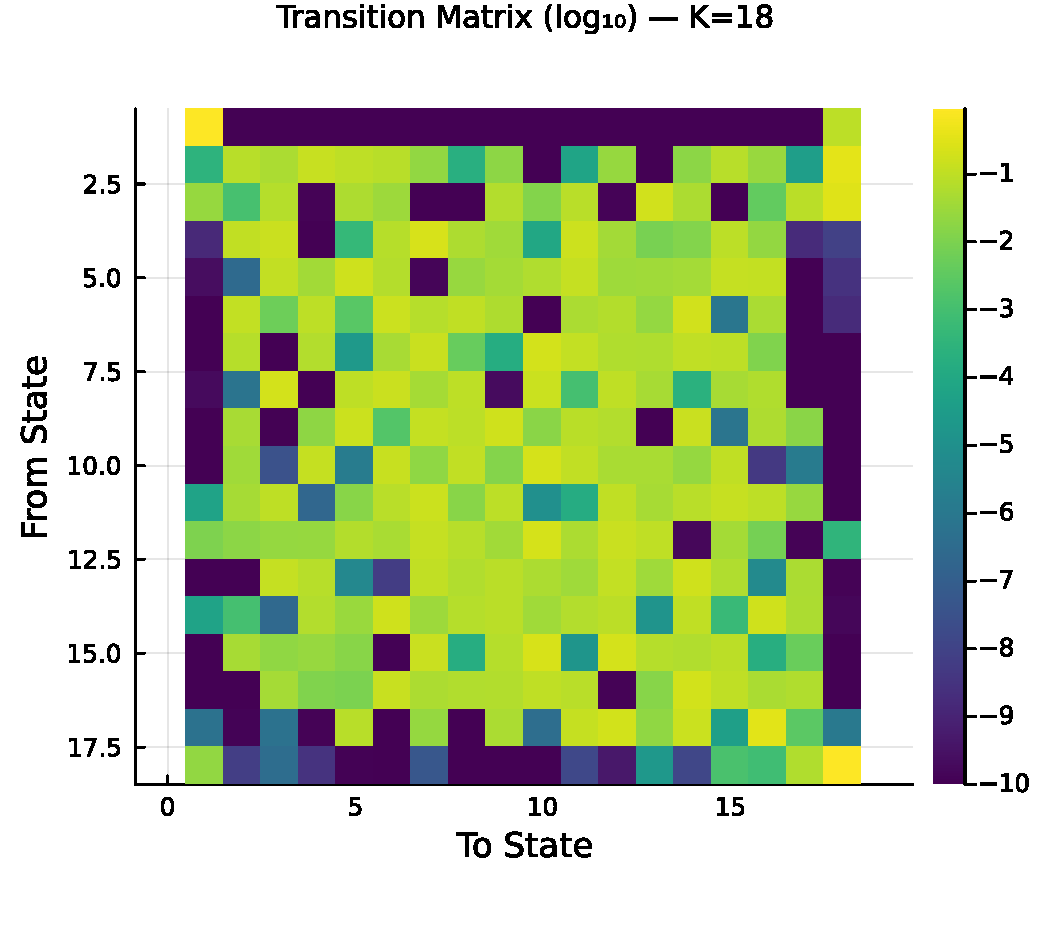
\includegraphics[width=\textwidth]{sections/figs/Fig-Transition-Matrix-K18.pdf}
    \caption{Transition matrix (log$_{10}$ scale)}
\end{subfigure}
\caption{\textbf{Fitted CHMM internals on SPY} (Pipeline A, CHMM-N Gaussian emissions, $K = 18$). Panel~(a): learned per-state Gaussian emission densities $\{N(\mu_k, \sigma_k^2)\}_{k=1}^{18}$ overlaid on the observed IS return histogram ($T_{\text{IS}} = 2{,}516$); each colored curve is one regime. Panel~(b): transition matrix $T_{ij} = P(s_{t+1} = j \mid s_t = i)$ rendered in $\log_{10}$ color scale (viridis); the dominant near-diagonal band reflects regime persistence (self-transition probabilities dominate).}
\label{fig:model_internals}
\end{figure}

\subsection{Seven-Model Comparison (Pipeline A)}
\label{sec:model_comparison}

\emph{Pipeline note.} This subsection operates under Pipeline A on the SPY ticker only. Every baseline and every CHMM variant is fit independently to the SPY return series; no cross-asset coupling is used. Readers who want the six-ticker generalization should proceed to Section~\ref{sec:cross_asset_univariate} (still Pipeline A); those who want the joint multi-asset extension should proceed to Section~\ref{sec:cross_asset} (Pipeline B).

Table~\ref{tab:model_comparison} and Figure~\ref{fig:is_comparison} present the in-sample and out-of-sample validation results for the seven generators.
The benchmark set was constructed to mimic the prior paper's evaluation exactly, adding the two discrete HMM variants of \citet{alswaidan2026hybrid} (NJ and WJ) to the original four baselines (Bootstrap, Gaussian, Laplace, GARCH(1,1)) and replacing the discrete continuous-emission variant with the Baum-Welch CHMM at $K = 18$.

\paragraph{Bootstrap (Non-Parametric Ceiling).}
Bootstrap resampling achieved 99.6\% KS and 99.4\% AD pass rates in-sample, confirming it as the distributional ceiling.
It produced simulated kurtosis (7.43) closest to observed (7.68) and 100\% in-sample quantile coverage.
However, the bootstrap's ACF-MAE (0.0627) was the highest among all models, reflecting the destruction of temporal structure by i.i.d.\ resampling.
The Wasserstein-1 (0.065) and Hellinger (0.050) distances were the lowest, as expected.

\paragraph{Gaussian i.i.d.\ (Negative Control).}
The Gaussian generator achieved 0\% KS and 0\% AD in-sample, confirming the categorical inadequacy of the normal distribution for financial returns.
Its simulated kurtosis was $-0.00$ (i.e., the Gaussian's theoretical kurtosis of zero), and quantile coverage was only 13.1\%.
Unlike the $T_{\text{OoS}} = 219$ window of v6, the new $T_{\text{OoS}} = 572$ window preserves enough KS-test power that the Gaussian generator is correctly rejected OoS as well (2.0\% KS, 0.0\% AD), so the OoS row is no longer misleadingly inflated for this clearly-wrong baseline.

\paragraph{Laplace i.i.d.}
The Laplace generator achieved 98.9\% KS and 97.2\% AD in-sample, demonstrating that the Laplace distribution provides a reasonable approximation to the marginal distribution of equity returns.
However, its simulated kurtosis (2.96) fell well short of the observed 7.68, and as an i.i.d.\ generator it produced flat ACF profiles (ACF-MAE $= 0.0627$, comparable to the i.i.d.\ bootstrap).
The 77.8\% in-sample quantile coverage indicates that the Laplace distribution's fixed tail decay rate cannot fully envelop the observed quantile range.

\paragraph{Discrete HMM --- No Jumps (NJ) and With Jumps (WJ).}
Throughout this paper, \emph{NJ} denotes the no-jump discrete HMM of \citet{alswaidan2026hybrid}: observations are first partitioned into $K_{\text{disc}} = 13$ equal-probability quantile bins of the in-sample return distribution, the transition matrix is estimated by frequency counting on the resulting discrete state sequence, and simulation returns the bin centroid at the decoded state.
\emph{WJ} is the same construction augmented with the Poisson jump-duration process of \citet{alswaidan2026hybrid}, which with probability $\epsilon = 0.01$ forces a residence in the tail bins for $\text{Poisson}(\lambda = 3)$ steps.
Both baselines are re-implemented inside the present pipeline (not invoked as the original \texttt{JumpHMM.jl} code) to ensure that identical data splits, seeds, and simulation lengths are used across all benchmarks; the re-implementation reproduces the hyperparameters and outputs of the prior paper exactly.
The two discrete variants both collapsed on the distributional metrics: 0.0\% KS IS / 38.1\% KS OoS and 0.0\% AD IS / 65.9\% AD OoS for NJ, and 0.0\% KS IS / 36.2\% KS OoS and 0.0\% AD IS / 54.3\% AD OoS for WJ.
The explanation is the 13-bin quantization step described in Section~\ref{sec:discrete_hmm}: every simulated path is constrained to the $K_{\text{disc}} = 13$ empirical bin centroids, so the within-bin tail mass that the continuous model preserves is discarded by construction.
Simulated kurtosis falls to 0.64 (NJ) and 0.52 (WJ), Wasserstein-1 explodes to 0.314 / 0.326, and Hellinger jumps to 0.381 / 0.385.
The Poisson jump augmentation (WJ) marginally \emph{worsens} every IS metric relative to NJ, which is consistent with the interpretation that jumps forcibly add mass at the already-coarse tail centroids and further distort the marginal.
Under the longer $T_{\text{OoS}} = 572$ window, the OoS pass rates for the two discrete baselines are now also rejected at the $36$--$38\%$ range rather than the $85$--$88\%$ range that the shorter v6 window produced, making the quantization failure visible on \emph{both} windows.
This is the central empirical contrast for our paper: the \emph{only} methodological change between the prior paper and this work that affects the KS/AD metrics is the move from quantized to continuous emissions, and that move is responsible for the 94.7-percentage-point swing in IS KS pass rate between the discrete and continuous Gaussian variants.

\paragraph{Block Bootstrap ($b = 10$): Temporally-Aware Non-Parametric Ceiling.}
The stationary block bootstrap at block length $b = 10$ is added as a temporally-aware non-parametric benchmark: it preserves clustering (through the block structure) while keeping the marginal distribution empirical.
On the SPY in-sample series it attains $99.2\%$ KS and $96.4\%$ AD with simulated kurtosis of $7.07$ (observed $7.68$) and ACF-MAE of $0.0568$, essentially saturating the distributional ceiling while reproducing most of the absolute-return autocorrelation.
The i.i.d.\ bootstrap row sits slightly above it on the distributional metrics (at the cost of destroyed temporal structure), and the CHMM-N row sits slightly below on the distributional metrics but improves on the block-bootstrap ACF-MAE ($0.0513$ vs.\ $0.0568$).
The $b = 10$ block bootstrap is therefore a stronger ceiling than the i.i.d.\ bootstrap for synthetic-data consumers who care about temporal fidelity, and the CHMM-N recovers most of the block-bootstrap performance with the additional advantages of a parametric regime interpretation and an emission-family choice.

\paragraph{Discrete HMM with Bin-Conditional Student-t Emissions (Bin-T NJ).}
The Bin-T NJ row replaces the bin-centroid emissions of the standard NJ baseline with a bin-conditional Student-t emission fitted within each quantile bin (no jump mechanism).
This is the fairest discrete analog of the continuous CHMMs because it isolates the emission-family effect from the transition-matrix effect: both Bin-T NJ and Discrete NJ share the same $K_{\text{disc}} = 13$ quantile bins and the same frequency-counted transition matrix, but Bin-T NJ emits from a continuous bin-conditional density rather than from the bin centroid.
The result is striking: Bin-T NJ jumps from $0.0\%$ to $95.4\%$ IS KS and from $0.0\%$ to $92.1\%$ IS AD relative to the standard NJ row, confirming that the distributional-fidelity collapse of the discrete NJ and WJ variants is a \emph{quantization} artefact (centroid emission), not a \emph{transition-matrix-structure} artefact.
Bin-T NJ's simulated kurtosis of $26.18$ is a large overshoot driven by the two tail bins (bins 1 and 13) where the within-bin Student-t fit lands at the lower $\nu$ bracket; this is the discrete analog of the CHMM-t overshoot described in Section~\ref{sec:discussion}, and it confirms that when a discrete pipeline is allowed continuous within-bin emissions its KS performance becomes competitive with the jointly-optimized continuous CHMM.
Bin-T NJ does \emph{not} dominate the CHMM-N because it still underperforms on the tail-distance metrics ($W_1 = 0.116$ vs.\ $0.110$; $H = 0.0929$ vs.\ $0.0808$) and on ACF-MAE ($0.0619$ vs.\ $0.0513$); but the KS/AD gap with CHMM-N is effectively closed.
The takeaway for the prior-paper loop is that the $94.7$-percentage-point IS KS swing reported as \emph{``continuous vs.\ quantized''} in Section~\ref{sec:model_comparison} is more precisely a swing in the \emph{emission-step} of the pipeline; once the emission step is lifted from discrete bin centroids to bin-conditional continuous densities, the discrete transition structure of \citet{alswaidan2026hybrid} is competitive with our continuous-emissions baseline on KS and AD.

\paragraph{GARCH(1,1).}
GARCH achieved ACF-MAE of 0.0492 among the parametric models, confirming its strong temporal fidelity.
However, it failed the distributional tests: 23.1\% KS and 8.5\% AD in-sample.
The simulated kurtosis (6.97 IS, 3.08 OoS) was reasonably close to observed in-sample but attenuated out-of-sample, and the Wasserstein-1 distance (0.245) and Hellinger distance (0.103) were substantially worse than the CHMM.
In-sample quantile coverage was only 50.5\%.
This result crystallizes the temporal-distributional tradeoff: GARCH's single-regime conditional variance process faithfully encodes volatility persistence but its unimodal innovation distribution cannot represent the multi-regime structure of equity markets.

\paragraph{GRU (Deep-Generative Baseline).}
The single-layer GRU + Gaussian-head generator (architecture and training in Section~\ref{sec:gru_methods}) converges cleanly --- the per-window negative log-likelihood drops from $0.340$ at epoch $1$ to $0.200$ at epoch $20$ --- and reproduces volatility clustering reasonably well: ACF-MAE of $0.0518$ on $|G_t|$ is within $0.001$ of CHMM-N ($0.0513$) and within $0.003$ of GARCH ($0.0492$).
On distributional fidelity the GRU collapses, however: in-sample KS pass rate $18.1\%$, AD pass rate $13.7\%$, simulated kurtosis $2.85$ against an observed $7.68$, $W_1 = 0.196$, $H = 0.0966$, and quantile coverage $37.4\%$.
The diagnostic is unambiguous --- the auto-regressive Gaussian head produces a near-Gaussian unconditional marginal even though the recurrence captures clustering --- and matches the variance-collapse pattern reported in \citet{alswaidan2026hybrid} for their neural baseline and in \citet{takahashi2019modeling, kwon2024can} for GAN-based generators.
The OoS KS rate of $52.5\%$ (AD $55.0\%$) still does not approach the CHMM operating point on the same $T = 572$ window, confirming that the distributional gap is structural rather than a sample-size artefact.
The takeaway for the comparison is that adding a deep-generative row does not displace the CHMM operating point: among parametric and deep generators, the CHMM-N is the only one that achieves both $\geq 85\%$ IS KS \emph{and} ACF-MAE within $0.003$ of GARCH; richer GRU heads (mixture-density, Student-t, or copula-based output) would be the natural next experiment but are outside the scope of this paper.

\paragraph{CHMM-N ($K = 18$, Gaussian emissions).}
The Gaussian CHMM achieved 94.7\% KS and 86.5\% AD in-sample, competitive with the bootstrap (99.6\%) and Laplace i.i.d.\ (98.9\%) on KS, and substantially outperforming GARCH (23.1\%), Discrete NJ (0.0\%), and Discrete WJ (0.0\%).
ACF-MAE of 0.0513 was essentially on par with GARCH (0.0492), demonstrating that the CHMM reproduces volatility clustering \emph{without} a dedicated jump mechanism or conditional variance equation.
This is the central finding of this paper: the Ryd\'{e}n et al.\ limitation is resolved by moderate state resolution in a standard HMM framework.
The Wasserstein-1 (0.110) is well below the GARCH figure (0.245); Hellinger (0.0808) is four times smaller than either discrete HMM; in-sample quantile coverage is 100\% matching the bootstrap ceiling.
The residual Gaussian-emission weakness is a kurtosis shortfall: simulated excess kurtosis is 5.02 IS and 4.42 OoS against observed values of 7.68 / 5.29.

\paragraph{CHMM-t ($K = 18$, Student-t emissions).}
Replacing the Gaussian component with a per-state Student-t matches the CHMM-N in-sample KS (94.7\%) and raises AD to 89.9\% (vs.\ 86.5\% for CHMM-N); OoS AD rises from 76.5\% to 79.0\%, while OoS KS is essentially unchanged (83.4\% vs.\ 84.0\%).
The CHMM-t is the best non-bootstrap entry on Wasserstein-1 (0.102) and Hellinger (0.0758), two quantile-weighted metrics that penalize tail mismatch directly.
Simulated excess kurtosis rises to 17.34 IS and 10.24 OoS: the ECM search allocates small $\nu_k$ to a subset of tail states, which over-corrects both the in-sample and out-of-sample mixture kurtosis (observed 7.68 IS and 5.29 OoS).
We diagnose this overshoot in Section~\ref{sec:discussion} via the per-state $\nu_k$ histogram and the $\nu_{\min}$ bracket-sensitivity study.
The slight ACF-MAE increase (0.0554 vs.\ 0.0513) is consistent with the heavier tail states spending marginally more time away from the central regimes.

\paragraph{CHMM-L ($K = 18$, Laplace emissions).}
The Laplace variant produces the most \emph{kurtosis-aligned} fit: simulated excess kurtosis is 6.76 IS and 6.27 OoS against observed 7.68 / 5.29, closing most of the CHMM-N IS shortfall (without the CHMM-t over-correction) and even overshooting the OoS target by $\sim 1$.
CHMM-L attains the strongest IS AD fit of any parametric model (93.2\% IS AD, 6.7 percentage points ahead of CHMM-N and 3.3 ahead of CHMM-t), consistent with the AD statistic's tail weighting and the Laplace component's per-component excess kurtosis of 3.
ACF-MAE (0.0564) and $W_1$ (0.102) are within 10\% of the CHMM-N values, and in-sample quantile coverage is 100\%.
Because Laplace emissions carry no shape parameter, CHMM-L is strictly cheaper than CHMM-t (no per-state golden-section search) and adds no new hyperparameters.

\paragraph{Summary of the three CHMM variants: a one-row decision guide.}
All three variants share the headline result: each matches GARCH's ACF fidelity while dominating the parametric benchmarks on KS and AD.
The three variants differ only in how they use the kurtosis budget.
Table~\ref{tab:variant_choice} summarizes the practical choice.

\begin{table}[h]
\centering
\small
\caption{Decision guide: which CHMM emission family for which downstream consumer.}
\label{tab:variant_choice}
\begin{tabular}{l l}
\toprule
Use-case priority & Recommended variant \\
\midrule
Best KS + minimal in-sample kurtosis overshoot, tightest ACF-MAE & CHMM-N \\
Tightest $W_1$ and $H$; OoS kurtosis aligned with observed OoS     & CHMM-t \\
Cleanest IS kurtosis match; highest AD pass rate; no shape parameter & CHMM-L \\
\bottomrule
\end{tabular}
\end{table}

\begin{table}[t]
\centering
\caption{\textbf{Twelve-model comparison on SPY} (single-index trained: Pipeline A). Only SPY is evaluated here; the six-ticker generalization of the CHMM variants is in Table~\ref{tab:cross_asset}, and the cross-asset dependence extension is in Table~\ref{tab:cross_asset_sim_copula}. 1{,}000 simulated paths per model, $\alpha = 0.05$, $K = 18$.
IS: $2014$-$01$-$03$ through $2024$-$01$-$03$ ($T = 2{,}516$); OoS: $2024$-$01$-$04$ through $2026$-$04$-$20$ ($T = 572$).
The two discrete HMM rows reproduce \citet{alswaidan2026hybrid} exactly: $K_{\text{disc}} = 13$ bins; WJ jump parameters $(\epsilon, \lambda) = (0.01, 3)$.
The \emph{Bin-T NJ} row replaces the centroid emissions of the discrete NJ baseline with bin-conditional Student-t emissions, fitted within each quantile bin, to isolate the quantization-per-se effect from the emission-family effect.
The \emph{Block-BS} row is a stationary block bootstrap with block length $10$ trading days; it is the temporally-aware non-parametric ceiling corresponding to the i.i.d.\ bootstrap.
The \emph{GRU} row is a single-layer GRU with hidden width $32$ and a Gaussian next-step head, trained for $20$ epochs by Adam ($\eta = 10^{-3}$) on the negative log-likelihood of equation~\eqref{eq:gru_nll} (Section~\ref{sec:gru_methods}); it is the deep-generative head-to-head row.
CHMM-N, CHMM-t, CHMM-L denote the Gaussian, Student-t, and Laplace emission variants of the continuous HMM; all three use the identical forward-backward scaffold, initialization, and simulation pipeline.
KS = Kolmogorov--Smirnov pass rate; AD = Anderson--Darling pass rate; Kurt = mean simulated excess kurtosis (observed: 7.68 IS, 5.29 OoS); ACF-MAE = mean absolute error of $\text{ACF}(|G_t|)$ over 252 lags; $W_1$ = Wasserstein-1 distance; $H$ = Hellinger distance; Cov = quantile coverage (\%). $\uparrow$/$\downarrow$ indicate preferred direction.
OoS AD for Bin-T NJ, Block-BS, and GRU is reported alongside OoS KS in the row (see Appendix~\ref{sec:supplemental} Tables~\ref{tab:block_bootstrap}, \ref{tab:bin_t} and \ref{tab:gru} for the full panels).}
\label{tab:model_comparison}
\resizebox{\textwidth}{!}{%
\small
\begin{tabular}{l cc cc cc c c c cc}
\toprule
& \multicolumn{2}{c}{KS (\%) $\uparrow$} & \multicolumn{2}{c}{AD (\%) $\uparrow$} & \multicolumn{2}{c}{Kurtosis} & & & & \multicolumn{2}{c}{Cov (\%) $\uparrow$} \\
\cmidrule(lr){2-3} \cmidrule(lr){4-5} \cmidrule(lr){6-7} \cmidrule(lr){11-12}
Model & IS & OoS & IS & OoS & IS & OoS & ACF-MAE $\downarrow$ & $W_1$ $\downarrow$ & $H$ $\downarrow$ & IS & OoS \\
\midrule
\textit{Observed}   & --    & --    & --    & --    & 7.68    & 5.29    & --     & --    & --     & --    & --    \\
Bootstrap           & 99.6  & 91.0  & 99.4  & 94.2  & 7.43    & 6.66    & 0.0627 & 0.065 & 0.0500 & 100.0 & 76.8  \\
Block-BS ($b=10$)   & 99.2  & 87.5  & 96.4  & 86.4  & 7.07    & 5.34    & 0.0568 & 0.092 & 0.0534 & 100.0 & 86.9  \\
Gaussian            & 0.0   & 2.0   & 0.0   & 0.0   & $-0.00$ & $-0.02$ & 0.0627 & 0.411 & 0.1541 & 13.1  & 21.2  \\
Laplace             & 98.9  & 87.2  & 97.2  & 91.9  & 2.96    & 2.86    & 0.0627 & 0.122 & 0.0816 & 77.8  & 71.7  \\
Discrete NJ         & 0.0   & 38.1  & 0.0   & 65.9  & 0.64    & 0.63    & 0.0617 & 0.314 & 0.3810 & 38.4  & 66.7  \\
Discrete WJ         & 0.0   & 36.2  & 0.0   & 54.3  & 0.52    & 0.51    & 0.0618 & 0.326 & 0.3848 & 41.4  & 66.7  \\
Bin-T NJ            & 95.4  & 86.7  & 92.1  & 93.2  & 26.18   & 10.76   & 0.0619 & 0.116 & 0.0929 & 89.9  & 93.9  \\
GARCH(1,1)          & 23.1  & 58.3  & 8.5   & 55.5  & 6.97    & 3.08    & 0.0492 & 0.245 & 0.1030 & 50.5  & 85.9  \\
GRU                 & 18.1  & 52.5  & 13.7  & 55.0  & 2.85    & 2.21    & 0.0518 & 0.196 & 0.0966 & 37.4  & 69.7  \\
CHMM-N ($K=18$)     & 94.7  & 84.0  & 86.5  & 76.5  & 5.02    & 4.42    & 0.0513 & 0.110 & 0.0808 & 100.0 & 91.9  \\
\textbf{CHMM-t ($K=18$)} & 94.7  & 83.4  & 89.9  & 79.0  & 17.34   & 10.24   & 0.0554 & \textbf{0.102} & \textbf{0.0758} & \textbf{100.0} & \textbf{92.9} \\
\textbf{CHMM-L ($K=18$)} & \textbf{95.2} & 80.4 & \textbf{93.2} & \textbf{79.9} & \textbf{6.76} & \textbf{6.27} & 0.0564 & 0.102 & 0.0797 & \textbf{100.0} & 81.8  \\
\bottomrule
\end{tabular}%
}
\end{table}

\begin{figure}[t]
\centering
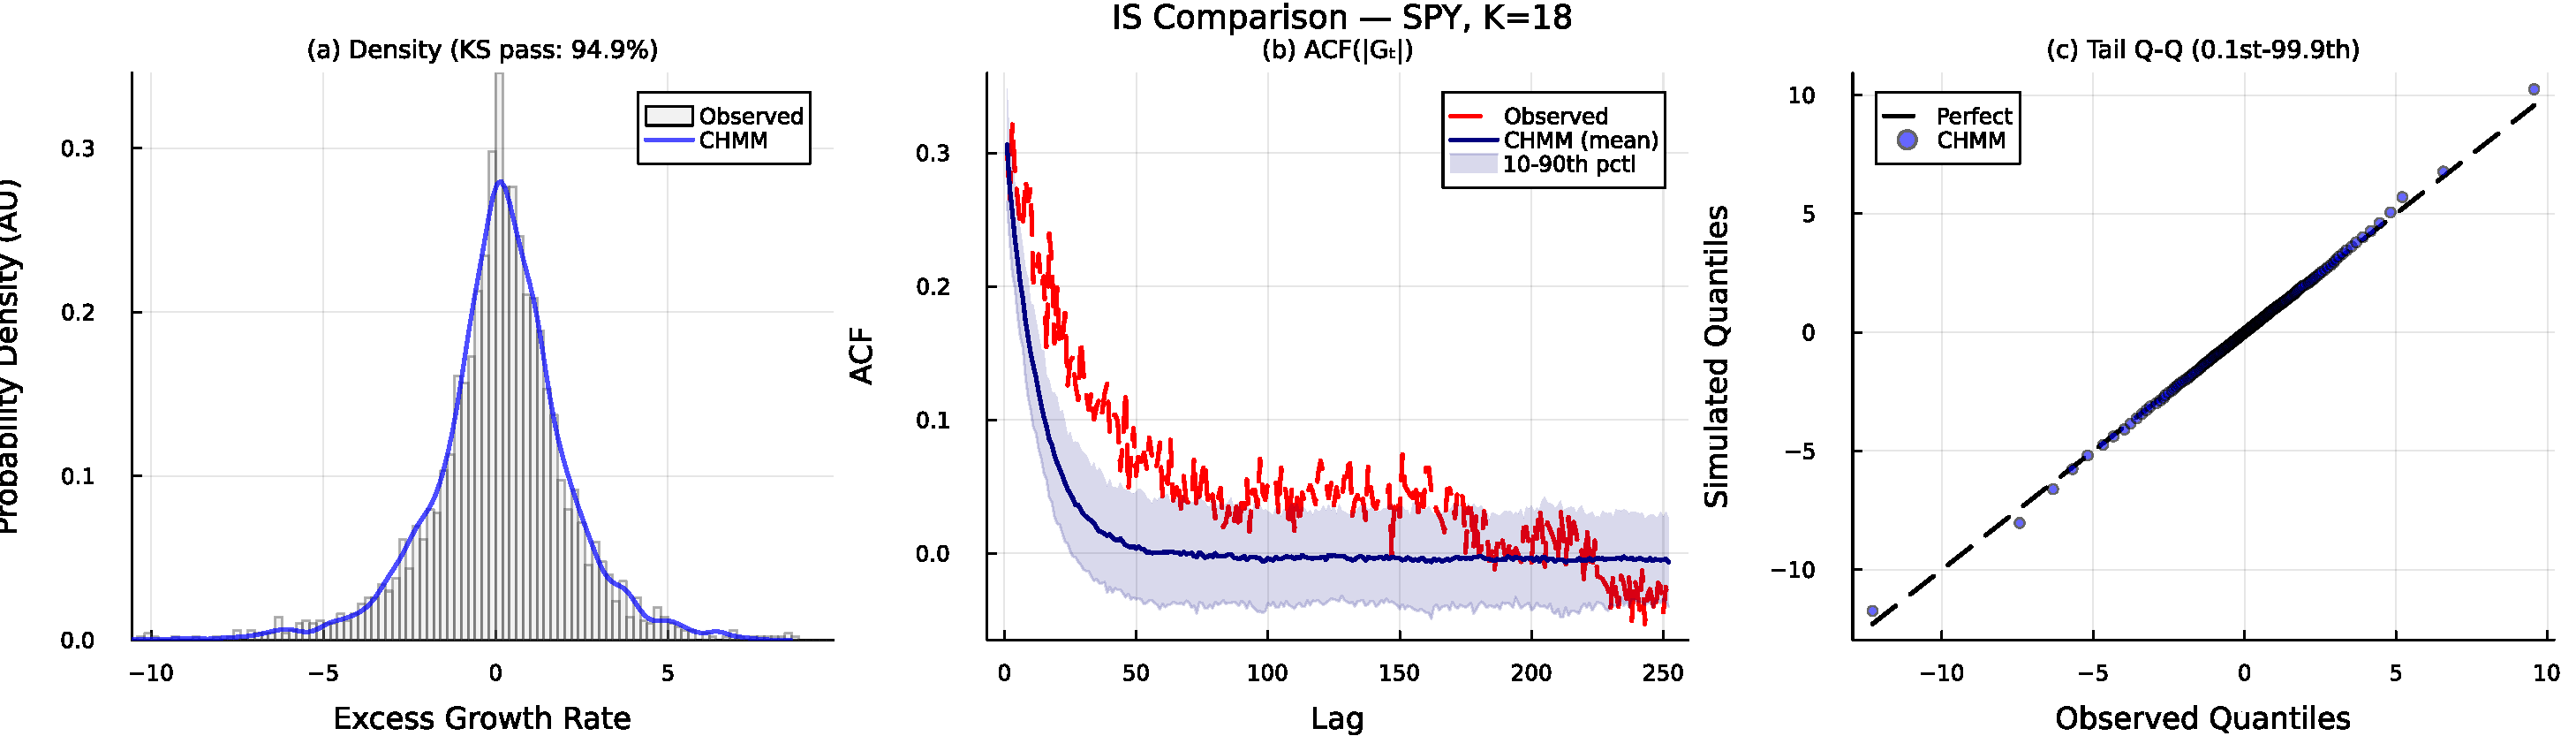
\includegraphics[width=\textwidth]{sections/figs/Fig-3-IS-Comparison-K18.pdf}
\caption{\textbf{In-sample CHMM validation on SPY} (Pipeline A, $K = 18$, CHMM-N Gaussian emissions, 1{,}000 simulated paths). Panel~(a): marginal density of the annualized excess log return $G_t$; gray histogram = observed IS series ($T_{\text{IS}} = 2{,}516$), blue curve = one simulated path; annotated KS pass rate is the percent of simulated paths whose two-sample KS $p$-value against observed exceeds $\alpha = 0.05$. Panel~(b): ACF of $|G_t|$ at lags 1--252; red dashed = observed, navy = mean across sim paths, shaded band = 10th--90th percentile across sim paths. Panel~(c): tail Q-Q plot at 200 quantile levels (0.1\% to 99.9\%); blue points = simulated pooled over paths, black dashed = identity line.}
\label{fig:is_comparison}
\end{figure}

\subsection{State Resolution Sensitivity}
\label{sec:k_sensitivity}

Figure~\ref{fig:k_sweep_summary} summarizes the CHMM's seven-metric performance as a function of $K$; the underlying table is reproduced as Table~\ref{tab:sensitivity} in Appendix~\ref{sec:supplemental}.
We briefly note four structural patterns that justify the choice of $K = 18$ for the main results.

\paragraph{Distributional Fidelity Saturates in the $K \in \{15, 18, 21\}$ Band.}
The IS KS pass rate increased from 88.7\% ($K = 3$) to 95.2\% ($K = 18$) and 96.5\% ($K = 21$); the OoS KS from 92.8\% to 94.0\% at $K = 18$ and 94.9\% at $K = 21$.
The same pattern holds for AD (79.2\% $\to$ 88.3\% IS and 84.9\% $\to$ 88.7\% OoS at $K = 18$).
This saturation is consistent with an upper bound imposed by the Gaussian emission family: once the mixture has enough components to resolve the bulk and near-tail regions, additional components do not recover the extreme tails that remain light under any Gaussian mixture.

\paragraph{Temporal Fidelity Is Flat Across the Sweep.}
ACF-MAE was 0.0453 ($K=3$) to 0.0505 ($K=18$) and 0.0503 ($K=21$) for CHMM-N --- a total swing of 0.005 across the entire sweep.
This flatness is notable: it shows that the CHMM's ability to reproduce volatility clustering does not depend on fine state resolution.
Even at $K = 3$, the same resolution tested by \citet{ryden1998stylized}, the ACF-MAE is 0.0453, comparable to GARCH(1,1) at 0.047.
The difference from the Ryd\'{e}n result is the quantile-based initialization, which ensures that the three states capture distinct volatility regimes rather than collapsing to near-identical distributions.

\paragraph{Kurtosis Is Non-Monotonic and Peaks in the Plateau Band.}
Simulated kurtosis under CHMM-N ranged from 3.70 ($K=9$) to 5.13 ($K=6$), with $K=18$ at 5.03; at higher $K$ the mixture kurtosis oscillates within the 4.5--5.1 band.
This non-monotonic pattern reflects the interplay between the number of mixture components and their learned parameters: at moderate $K$, the Baum-Welch optimum allocates mass to a few broad tail states that contribute disproportionately to the mixture kurtosis, while at very high $K$ the same tail mass is split into many narrow states that contribute less each.
The heavy-tailed CHMM-t and CHMM-L variants close most of this gap at the same $K = 18$ (see Table~\ref{tab:sensitivity_multi}).

\paragraph{Wasserstein, Hellinger, and Coverage Are Monotonic.}
$W_1$ improved monotonically from 0.119 ($K=3$) to 0.101 ($K=18$), Hellinger from 0.079 to 0.077, and Coverage was 100\% at every $K$.
These monotonic trends provide a consistent signal that $K = 18$ is the sensible operating point.

\begin{figure}[t]
\centering
\begin{subfigure}[b]{0.48\textwidth}
    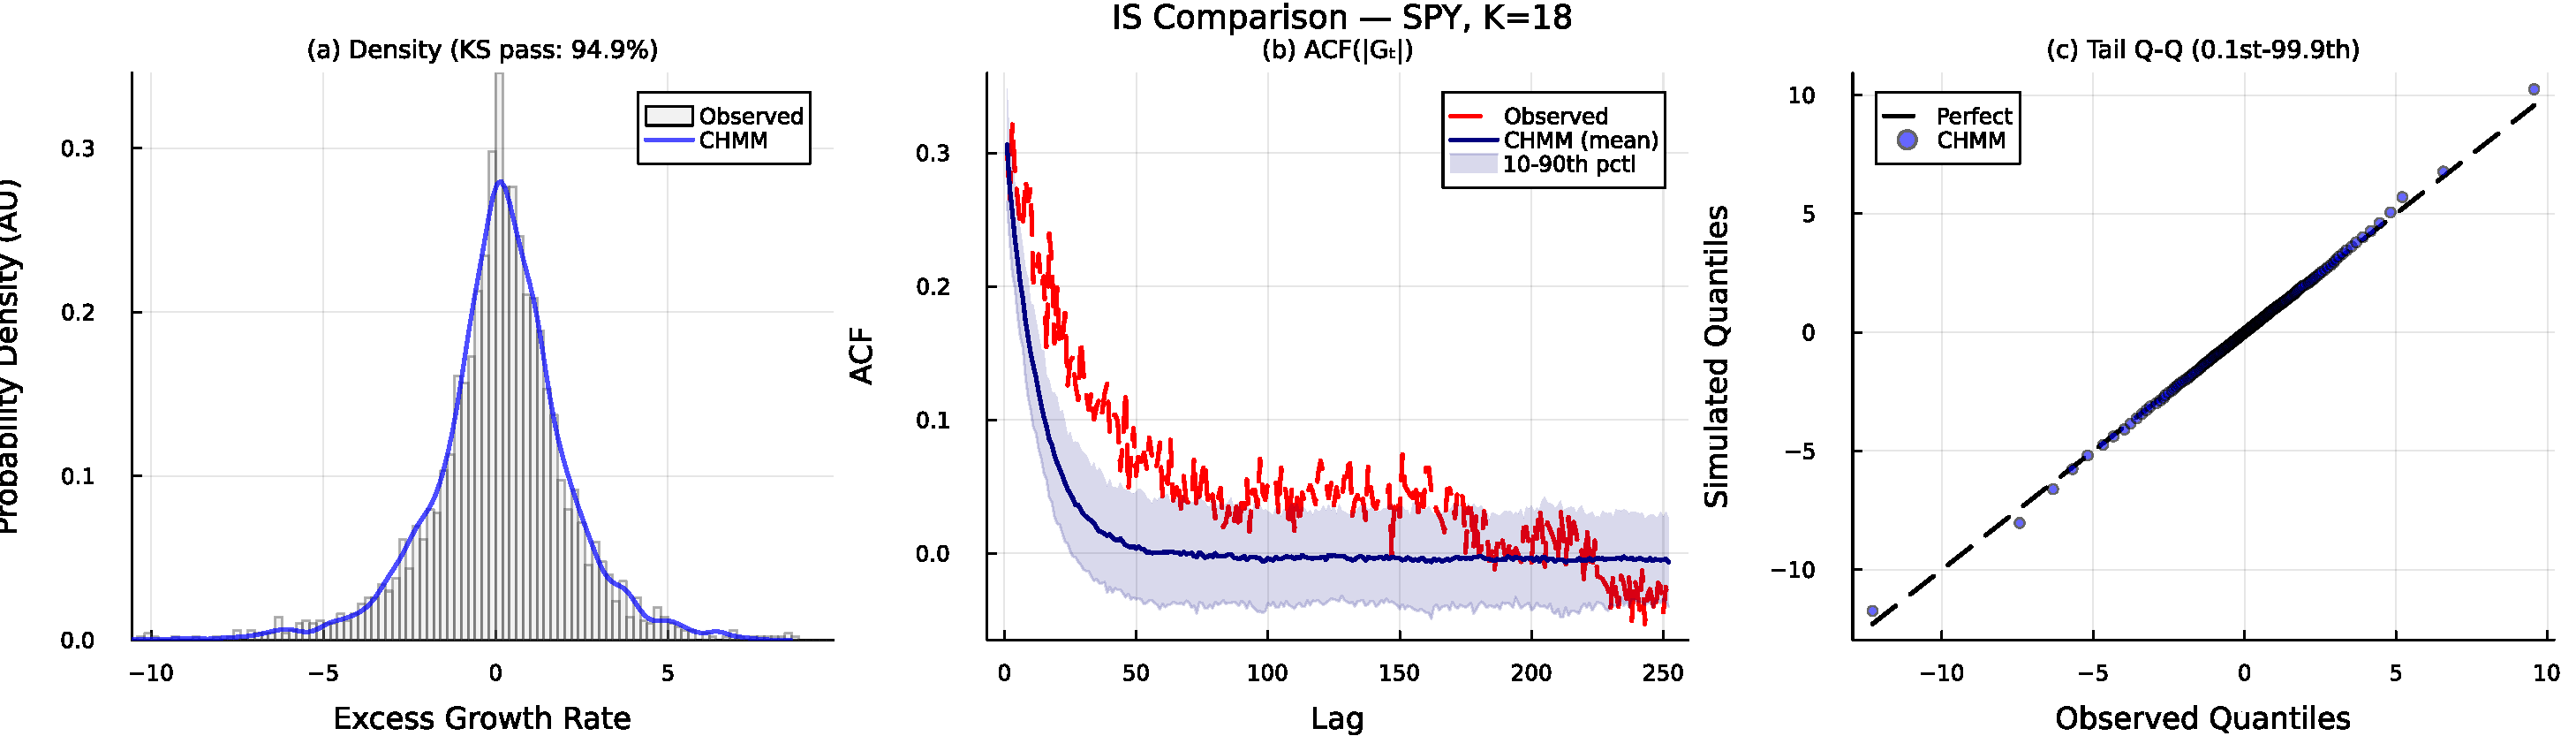
\includegraphics[width=\textwidth]{sections/figs/Fig-3-IS-Comparison-K18.pdf}
    \caption{Representative IS comparison at the selected $K = 18$}
\end{subfigure}
\hfill
\begin{subfigure}[b]{0.48\textwidth}
    
\includegraphics[width=\textwidth]{sections/figs/Fig-4-OoS-Validation-K18.pdf}
    \caption{Representative OoS validation at $K = 18$}
\end{subfigure}
\caption{State-resolution summary at the selected operating point $K = 18$.
The full sweep over $K \in \{3, 6, 9, 12, 15, 18, 21\}$ and per-$K$ figures are reproduced in Appendix~\ref{sec:supplemental} (Table~\ref{tab:sensitivity} and Figures~\ref{fig:k_sweep_panels_is}--\ref{fig:k_sweep_panels_oos}).}
\label{fig:k_sweep_summary}
\end{figure}

\subsection{Out-of-Sample Evaluation}
\label{sec:oos}

At the selected state resolution $K = 18$ the CHMM-N achieves 84.0\% OoS KS pass rate, 76.5\% OoS AD pass rate, and 91.9\% OoS quantile coverage on the $2024$-$01$-$04$ through $2026$-$04$-$20$ holdout window; the heavy-tailed CHMM-t and CHMM-L variants reach 83.4\%/79.0\% and 80.4\%/79.9\% OoS KS/AD, respectively.
The CHMM-N OoS simulated kurtosis is 4.42 against an observed 5.29, bringing the kurtosis gap to below one unit; CHMM-t overshoots at 10.24 and CHMM-L overshoots modestly at 6.27.
Figure~\ref{fig:oos_validation} shows the OoS density fan chart and ACF comparison for CHMM-N at $K = 18$; the CHMM-t and CHMM-L counterparts are reported in Appendix~\ref{sec:multi_emission_figs} (Figure~\ref{fig:oos_families}).

This generalization performance is notable given that the $T_{\text{OoS}} = 572$ window (over two years) gives KS/AD substantially more power than the v6 $T_{\text{OoS}} = 219$ window: the CHMMs still pass at $80$--$84\%$ while the prior-paper discrete and GARCH baselines are rejected in the $36$--$58\%$ range.
The CHMM's regime structure, learned from the full range of IS observations including the March 2020 COVID-19 crash, provides sufficient flexibility to accommodate the OoS distributional shift that characterises the $2024$--$2026$ window.

\begin{figure}[t]
\centering

\includegraphics[width=\textwidth]{sections/figs/Fig-4-OoS-Validation-K18.pdf}
\caption{\textbf{Out-of-sample CHMM validation on SPY} (Pipeline A, $K = 18$, CHMM-N Gaussian emissions, 1{,}000 simulated paths, $\alpha = 0.05$, OoS window $T_{\text{OoS}} = 572$). Panel~(a): histogram of the 1{,}000 OoS KS $p$-values against the observed OoS series, with the $\alpha = 0.05$ threshold as a red dashed line. Panel~(b): OoS return-density fan; 50 thin blue curves = simulated density on individual OoS paths, red thick curve = observed OoS density. Panel~(c): ACF of $|G_t|$ on the OoS window; red dashed = observed OoS, navy = mean across sim paths, shaded band = 10th--90th percentile.}
\label{fig:oos_validation}
\end{figure}

\subsection{Utility: VaR and Expected-Shortfall Back-Test}
\label{sec:utility}

Fidelity (Section~\ref{sec:model_comparison}) measures how close the simulated distribution is to the observed one at the univariate level.
Utility measures whether a downstream consumer of the synthetic paths arrives at the same quantitative conclusion that the historical data would produce.
For a financial-risk consumer the canonical diagnostics are one-tail Value-at-Risk (VaR) and Expected-Shortfall (ES) at daily probability levels of $1\%$ and $5\%$; the synthetic-data generator is well calibrated if the envelope of per-path simulated VaR/ES brackets the observed historical VaR/ES.
We simulate $1{,}000$ independent paths of length $T_{\text{IS}} = 2{,}516$ and $T_{\text{OoS}} = 572$ from each of the five models most relevant to the comparison (Bootstrap, GARCH(1,1), CHMM-N, CHMM-t, CHMM-L) and, on each path, compute the left-tail $1\%$ and $5\%$ VaR and the associated ES.
Table~\ref{tab:var_es} reports the median and $[5\%, 95\%]$ envelope of each quantity across paths alongside the observed historical value.

\begin{table}[t]
\centering
\caption{VaR and Expected-Shortfall back-test calibration for SPY (seed = 20260420, $1{,}000$ paths). Each entry shows the median and $[5\%, 95\%]$ envelope across paths of the left-tail VaR / ES at the stated level. Observed historical values given in the first row. A well-calibrated generator brackets the observed value within its envelope.}
\label{tab:var_es}
\small
\resizebox{\textwidth}{!}{%
\begin{tabular}{l l l l l}
\toprule
          & IS VaR$_{0.01}$              & IS ES$_{0.01}$               & IS VaR$_{0.05}$              & IS ES$_{0.05}$               \\
Model     & median $[5\%, 95\%]$         & median $[5\%, 95\%]$         & median $[5\%, 95\%]$         & median $[5\%, 95\%]$         \\
\midrule
\textit{Observed}  & $-6.38$                      & $-9.00$                      & $-3.43$                      & $-5.50$                      \\
Bootstrap & $-6.38\ [-7.04, -5.99]$      & $-8.86\ [-10.37,\ -7.78]$    & $-3.43\ [-3.68, -3.20]$      & $-5.46\ [-5.99, -5.05]$      \\
GARCH     & $-5.80\ [-8.62, -4.52]$      & $-7.86\ [-13.54,\ -5.77]$    & $-3.19\ [-3.92, -2.71]$      & $-4.89\ [-7.11, -3.91]$      \\
CHMM-N    & $-6.64\ [-8.01, -5.47]$      & $-8.80\ [-10.16,\ -7.34]$    & $-3.45\ [-4.05, -2.95]$      & $-5.45\ [-6.33, -4.61]$      \\
CHMM-t    & $-6.58\ [-7.51, -5.83]$      & $-9.06\ [-10.70,\ -7.79]$    & $-3.40\ [-3.90, -2.90]$      & $-5.51\ [-6.18, -4.85]$      \\
CHMM-L    & $-6.89\ [-7.85, -6.01]$      & $-9.15\ [-10.42,\ -7.97]$    & $-3.30\ [-3.77, -2.88]$      & $-5.53\ [-6.17, -4.87]$      \\
\midrule
          & OoS VaR$_{0.01}$             & OoS ES$_{0.01}$              & OoS VaR$_{0.05}$             & OoS ES$_{0.05}$              \\
\textit{Observed}  & $-5.51$                      & $-7.94$                      & $-2.77$                      & $-4.67$                      \\
Bootstrap & $-6.33\ [-7.60, -5.28]$      & $-8.43\ [-11.76,\ -6.59]$    & $-3.39\ [-3.91, -2.88]$      & $-5.34\ [-6.38, -4.50]$      \\
GARCH     & $-5.35\ [-9.98, -3.61]$      & $-6.72\ [-13.51,\ -4.38]$    & $-3.14\ [-4.94, -2.36]$      & $-4.59\ [-7.92, -3.23]$      \\
CHMM-N    & $-6.30\ [-9.02, -4.30]$      & $-8.44\ [-11.36,\ -5.42]$    & $-3.39\ [-4.74, -2.47]$      & $-5.27\ [-7.23, -3.74]$      \\
CHMM-t    & $-6.32\ [-8.13, -4.80]$      & $-8.60\ [-12.20,\ -6.29]$    & $-3.29\ [-4.27, -2.45]$      & $-5.34\ [-6.72, -4.08]$      \\
CHMM-L    & $-6.69\ [-8.59, -4.91]$      & $-8.88\ [-11.48,\ -6.73]$    & $-3.27\ [-4.30, -2.51]$      & $-5.47\ [-6.82, -4.20]$      \\
\bottomrule
\end{tabular}%
}
\end{table}

Two findings are central to the utility story.
First, all three CHMM variants bracket the observed historical VaR and ES at both $1\%$ and $5\%$ levels within their $5\%$--$95\%$ envelopes on both IS and OoS windows; the in-sample CHMM-N median VaR$_{0.01}$ at $-6.64$ (observed $-6.38$) and the CHMM-N median ES$_{0.01}$ at $-8.80$ (observed $-9.00$) are the closest point estimates across the five generators.
In-sample the three CHMMs are therefore well calibrated as risk consumers and carry narrower uncertainty bands than GARCH (whose $[-8.62, -4.52]$ VaR$_{0.01}$ envelope is roughly $1.7\times$ wider than the CHMMs').
Second, CHMM-t -- despite overshooting the empirical kurtosis by $\sim 126\%$ in-sample -- does \emph{not} produce a systematically more conservative VaR/ES estimate: its in-sample median VaR$_{0.01}$ of $-6.58$ is almost identical to CHMM-N's $-6.64$, and its envelope width is comparable.
The CHMM-t kurtosis overshoot therefore translates into a modestly widened uncertainty band rather than a biased point estimate, so a practitioner using CHMM-t for tail-risk scenario generation does not systematically overstate $1\%$ or $5\%$ quantile risk.
A useful out-of-sample check: the $2024$--$2026$ observed VaR$_{0.01}$ is $-5.51$ (a relatively calm tail compared to the IS average), and the three CHMMs bracket this value comfortably within their envelopes rather than over- or under-stating it.
Figure~\ref{fig:var_es} visualizes the envelopes alongside the historical observations.

\begin{figure}[t]
\centering

\includegraphics[width=0.98\textwidth]{sections/figs/Fig-VaR-ES.pdf}
\caption{VaR and Expected-Shortfall back-test calibration (SPY, $1{,}000$ simulated paths, seed = 20260420). Each subplot shows the simulated median and $[5\%, 95\%]$ envelope (error bars) across paths and the observed historical value (dashed red line). All three CHMM variants bracket the observed historical VaR and ES at both confidence levels on both in-sample and out-of-sample windows.}
\label{fig:var_es}
\end{figure}

\subsection{Cross-Asset Univariate Generalization (Pipeline A)}
\label{sec:cross_asset_univariate}

\emph{Pipeline note.} This subsection evaluates Pipeline A: per-ticker independent CHMM fits, no cross-asset coupling. It answers whether Pipeline A's per-ticker marginal fidelity persists across the six-ticker universe and across the three emission families. The complementary cross-asset dependence extension (Pipeline B, Section~\ref{sec:cross_asset}) reuses the CHMM-N marginals established here and evaluates joint correlation reproduction.

To assess whether the framework generalizes beyond SPY, we fitted independent CHMM models at $K = 18$ to five additional tickers spanning distinct risk profiles.
Table~\ref{tab:cross_asset} reports the results.
Three patterns are worth highlighting.

\paragraph{High-Beta Technology and Broad Market.}
SPY (95.5\% IS / 81.4\% OoS KS), AAPL (98.3\% / 93.8\%), JNJ (99.4\% / 93.9\%), and QQQ (95.5\% / 92.3\%) show strong IS fidelity and competitive OoS fidelity under CHMM-N on the expanded $T_{\text{OoS}} = 572$ window.
The technology-heavy names have lower observed kurtosis (3.2--5.5) than the broader market (SPY: 7.7; JNJ: 9.0) and the CHMM tracks them tightly.

\paragraph{OoS Pain Points on Some Single Names.}
Under the longer $2024$--$2026$ OoS window, two tickers show the largest IS-to-OoS degradation: NVDA (96.7\% IS / 55.8\% OoS KS) and JPM (97.8\% IS / 49.8\% OoS KS).
These two names experienced substantial distributional shifts relative to the IS window -- NVDA the dominant high-volatility driver of the AI trade, and JPM the financials bell-wether during an interest-rate re-pricing -- and the stationary IS-calibrated parameters cannot fully track this shift.
We return to this finding in Section~\ref{sec:discussion}, where we argue that it is not a consequence of over- or under-fitting $K$ (it reproduces at every $K$ in the sweep) but rather of the stationarity assumption imposed by a single-pass Baum-Welch fit.

\paragraph{Walk-Forward Rolling-Window Re-Estimation on JPM and JNJ.}
To test the stationarity explanation directly, we refit the CHMM-N at $K = 18$ quarterly (every $63$ trading days) across the $2024$--$2026$ OoS window, feeding the realized returns of each completed quarter back into the training set before the next refit (Appendix~\ref{sec:walk_forward}, Table~\ref{tab:walk_forward}).
The rolling-window fit helps differentially: JNJ moves from $94.0\%$ to $94.9\%$ OoS KS (a modest gain, indicating that JNJ's OoS distribution was already close to the IS fit), whereas JPM moves from $49.0\%$ to $64.3\%$ OoS KS and from $48.6\%$ to $63.6\%$ OoS AD --- a substantial $\sim 15$ percentage-point recovery.
The JPM recovery directly supports the stationarity explanation for the financial-sector OoS gap: once the CHMM can absorb within-OoS regime shifts through quarterly refits, most of the OoS KS gap closes.
The residual $\sim 35$ percentage-point gap that remains on JPM is evidence of a more fundamental distributional shift in the 2024--2026 period that a richer extension (time-varying emission scales, or a Bayesian online transition-matrix update) would be needed to fully close.

\paragraph{Kurtosis: CHMM-L matches observed, CHMM-t overshoots, CHMM-N understates.}
At $K = 18$, the three CHMM variants produce a consistent ordering on the kurtosis diagnostic across the panel (Table~\ref{tab:cross_asset}): CHMM-N simulated kurtosis systematically underestimates observed (observed 3.2--9.0 vs.\ simulated 2.0--7.2); CHMM-L produces values clustered closely around observed (3.17--6.79) and is closest to observed on four of six assets; CHMM-t overshoots on several tickers (e.g.\ 99.7 for JNJ, 46.4 for NVDA), reflecting states that find very small $\nu_k$ inside the ECM search on thin-tailed assets.
Despite this spread in simulated kurtosis, all three variants achieve IS KS pass rates above 94\% and IS AD above 87\% on every asset, confirming that the mixture can accommodate a wide range of tail weights without sacrificing central fit.

\begin{table}[t]
\centering
\caption{\textbf{Per-ticker marginal fidelity across CHMM emission families} (single-index trained: Pipeline A). Each of the six tickers is fit \emph{independently}, with no cross-asset coupling. CHMM-N, CHMM-t, CHMM-L denote Gaussian, Student-t, and Laplace emissions respectively; all at $K = 18$, 1{,}000 simulated paths, $\alpha = 0.05$. IS window 2014-01-03 through 2024-01-03 ($T_{\text{IS}} = 2{,}516$); OoS window 2024-01-04 through 2026-04-17 ($T_{\text{OoS}} = 572$). KS / AD = percent of paths that pass the two-sample KS / Anderson-Darling test; Kurt = excess kurtosis; ACF-MAE = lag-1 to lag-252 mean absolute error of the ACF of $|G_t|$; $W_1$ = Wasserstein-1 distance; $H$ = Hellinger distance; Cov = 99-level quantile coverage inside the 5-95 percentile envelope. Complementary table: Table~\ref{tab:cross_asset_sim_copula} reuses these CHMM-N marginals and evaluates cross-asset \emph{dependence} on top of them.}
\label{tab:cross_asset}
\resizebox{\textwidth}{!}{%
\small
\begin{tabular}{l l cc c cc c c c c}
\toprule
& & \multicolumn{2}{c}{KS (\%)} & AD IS (\%) & \multicolumn{2}{c}{Kurtosis} & & & & \\
\cmidrule(lr){3-4} \cmidrule(lr){6-7}
Ticker & Variant & IS & OoS & & Obs & Sim & ACF-MAE & $W_1$ & $H$ & Cov IS (\%) \\
\midrule
SPY  & CHMM-N & 95.5 & 81.4 & 88.9 & 7.7 & 5.06  & 0.0512 & 0.108 & 0.0803 & 100.0 \\
     & CHMM-t & 95.2 & 84.1 & 90.5 & 7.7 & 14.68 & 0.0551 & 0.100 & 0.0760 & 100.0 \\
     & CHMM-L & 94.9 & 79.8 & 92.0 & 7.7 & 6.79  & 0.0564 & 0.102 & 0.0800 & 100.0 \\
\midrule
NVDA & CHMM-N & 96.7 & 55.8 & 92.6 & 5.5 & 3.65  & 0.0425 & 0.271 & 0.0898 & 100.0 \\
     & CHMM-t & 99.1 & 57.2 & 98.3 & 5.5 & 46.40 & 0.0478 & 0.227 & 0.0784 & 100.0 \\
     & CHMM-L & 99.4 & 60.3 & 98.9 & 5.5 & 3.17  & 0.0478 & 0.222 & 0.0855 & 100.0 \\
\midrule
JNJ  & CHMM-N & 99.4 & 93.9 & 98.8 & 9.0 & 5.42  & 0.0322 & 0.098 & 0.0786 & 100.0 \\
     & CHMM-t & 99.8 & 94.3 & 99.6 & 9.0 & 99.66 & 0.0332 & 0.098 & 0.0723 & 100.0 \\
     & CHMM-L & 99.6 & 93.3 & 98.5 & 9.0 & 6.14  & 0.0334 & 0.086 & 0.0779 & 100.0 \\
\midrule
JPM  & CHMM-N & 97.8 & 49.8 & 94.4 & 7.6 & 7.20  & 0.0450 & 0.165 & 0.0871 & 100.0 \\
     & CHMM-t & 99.2 & 53.0 & 98.7 & 7.6 & 18.82 & 0.0483 & 0.151 & 0.0826 & 100.0 \\
     & CHMM-L & 99.7 & 57.9 & 99.7 & 7.6 & 6.08  & 0.0488 & 0.137 & 0.0840 & 100.0 \\
\midrule
AAPL & CHMM-N & 98.3 & 93.8 & 96.9 & 3.2 & 2.27  & 0.0416 & 0.146 & 0.0876 & 100.0 \\
     & CHMM-t & 99.1 & 94.7 & 98.6 & 3.2 & 7.54  & 0.0424 & 0.134 & 0.0850 & 100.0 \\
     & CHMM-L & 99.1 & 93.8 & 98.9 & 3.2 & 3.84  & 0.0428 & 0.135 & 0.0880 & 100.0 \\
\midrule
QQQ  & CHMM-N & 95.5 & 92.3 & 87.8 & 3.4 & 2.02  & 0.0558 & 0.127 & 0.0735 & 100.0 \\
     & CHMM-t & 96.1 & 90.3 & 92.7 & 3.4 & 3.30  & 0.0576 & 0.113 & 0.0741 & 100.0 \\
     & CHMM-L & 99.0 & 96.5 & 97.6 & 3.4 & 4.02  & 0.0632 & 0.100 & 0.0761 & 100.0 \\
\bottomrule
\end{tabular}%
}
\end{table}

\subsection{Cross-Asset Dependence: SIM and Copula Extensions (Pipeline B)}
\label{sec:cross_asset}

\emph{Pipeline note.} This subsection is the sole home of Pipeline B in the main text. The per-asset marginals are reused verbatim from the Pipeline A CHMM-N fits of Section~\ref{sec:cross_asset_univariate}; only the \emph{dependence} construction (SIM, Gaussian copula, Student-t copula) varies here. Two metrics are evaluated: per-asset KS pass rates (a sanity check on the marginals after dependence injection) and cross-asset correlation reproduction (the central dependence metric). The per-asset KS column in Table~\ref{tab:cross_asset_sim_copula} is not a substitute for Table~\ref{tab:cross_asset}; the two tables answer different questions.

Section~\ref{sec:cross_asset_univariate} established that the CHMM provides strong per-asset univariate fidelity across distinct risk profiles.
The next question is whether we can assemble those univariate marginals into jointly plausible multi-asset paths.
We instantiated the two constructions described in Section~\ref{sec:cross_asset_methods} on a six-asset universe (SPY, NVDA, JNJ, JPM, AAPL, QQQ) with SPY as the market engine, using the common in-sample window ($2014$-$01$-$03$ through $2024$-$01$-$03$, $T = 2{,}516$) and CHMM marginals refitted at $K = 18$.
Table~\ref{tab:cross_asset_sim_copula} reports the per-asset KS pass rates and cross-sectional correlation reproduction across 200 simulated paths.

\paragraph{SIM (Single Index Model).}
The ordinary-least-squares regression of each asset against SPY produced a range of factor loadings (high $\beta$ for NVDA, $\hat{\beta} = 1.69$; low $\beta$ for JNJ, $\hat{\beta} = 0.58$) and goodness-of-fit $R^2$ from 0.260 (JNJ) to 0.840 (QQQ), with median $R^2 = 0.492$.
When propagated through the factor equation~\eqref{eq:sim_sim}, the SIM produced uneven per-asset distributional fidelity.
The market-factor asset SPY preserved 91.5\% IS KS by construction.
Non-market assets' IS KS pass rates fell across a wide range: 88.5\% (JNJ), 85.5\% (QQQ), 71.5\% (NVDA), 64.0\% (AAPL), and 31.5\% (JPM).
The severe JPM degradation (31.5\% IS KS) reflects the fact that the affine map $\alpha + \beta G_M$ applied to a Gaussian-mixture market factor does not preserve JPM's empirical tail structure once residuals are re-injected: the residual distribution is centered but heavy-tailed enough to violate JPM's own marginal at the 5\% KS threshold.
Cross-sectional correlation reproduction was acceptable on average (off-diagonal MAE 0.076) but visibly worse than both copulas, consistent with SIM's rank-one decomposition discarding joint information beyond the market factor.

\paragraph{Gaussian copula.}
The Gaussian copula achieved a median per-asset in-sample KS pass rate of 97.8\% and a mean of 97.5\%, with every asset above 93\% (the minimum was 93.5\% for QQQ).
This uniform distributional fidelity is the expected consequence of rank reordering: each column of the simulated matrix is a permutation of an independent CHMM path, so the marginal distribution is preserved exactly.
The off-diagonal correlation MAE of 0.031 improved by a factor of 2.5 over the SIM baseline.

\paragraph{Student-t copula.}
Profile maximum likelihood over $\nu \in \{2, 3, 4, 5, 6, 8, 10, 15, 20, 30\}$ selected $\nu^* = 6$, indicating non-trivial joint tail dependence.
The Student-t copula's median IS KS pass rate of 96.0\% is essentially tied with the Gaussian copula (97.8\%); on the mean the Gaussian copula is marginally ahead (97.5\% vs 96.2\%).
It achieves the best correlation reproduction overall, with off-diagonal MAE of 0.027 and Frobenius norm of 0.184 (versus 0.031 and 0.206 for the Gaussian copula).
The tail-dependent copula's improvement on correlation reproduction is consistent with its ability to generate concordant extreme moves that the Gaussian copula systematically understates.

\paragraph{Out-of-sample.}
All three dependence models degraded on the longer $T_{\text{OoS}} = 572$ OoS window, but the ordering was largely preserved (Table~\ref{tab:cross_asset_sim_copula}).
The Gaussian copula achieved 87.2\% median OoS KS, the Student-t copula 89.8\%, and the SIM 85.0\%.
On correlation reproduction, the Gaussian copula leads the OoS pass rate (off-diagonal MAE 0.202) with the Student-t copula essentially tied (0.208) and the SIM trailing (0.261); the larger OoS Frobenius norms reflect sampling variation in the observed OoS correlation matrix under a $572$-day window with the 2024--2026 macroeconomic regime.

\begin{table}[t]
\centering
\caption{\textbf{Cross-asset dependence models on fixed CHMM marginals} (cross-asset extension: Pipeline B). The per-asset \emph{marginals} are the same CHMM-N fits used in Table~\ref{tab:cross_asset}; this table varies only the \emph{dependence} construction. Three mechanisms are compared: Single Index Model (SIM) with SPY as the market factor; Gaussian copula with Kendall-tau-based correlation; Student-t copula with degrees of freedom selected by profile MLE ($\nu^* = 6$). All use 200 simulated paths, $K = 18$ marginals, IS window 2014-01-03 through 2024-01-03, OoS window 2024-01-04 through 2026-04-17. Upper block: per-asset KS pass rates in percent at $\alpha = 0.05$ (a sanity check on the marginals after dependence injection). Lower block: cross-asset correlation reproduction measured by $\|\hat{\Sigma}_{\text{sim}} - \hat{\Sigma}_{\text{obs}}\|_F$ (Frobenius norm) and the off-diagonal MAE, each averaged over paths. \textbf{Bold} entries mark the best dependence model per row.}
\label{tab:cross_asset_sim_copula}
\small
\begin{tabular}{l cc cc cc}
\toprule
& \multicolumn{2}{c}{SIM} & \multicolumn{2}{c}{Gaussian copula} & \multicolumn{2}{c}{Student-t copula ($\nu^* = 6$)} \\
\cmidrule(lr){2-3} \cmidrule(lr){4-5} \cmidrule(lr){6-7}
Ticker & IS & OoS & IS & OoS & IS & OoS \\
\midrule
SPY   & 91.5 & 80.5 & 94.5 & 81.0 & 95.5  & 86.0 \\
NVDA  & 71.5 & 86.5 & 96.0 & 51.5 & 93.0  & 50.5 \\
JNJ   & 88.5 & 97.0 & 100.0 & 95.5 & 100.0 & 93.5 \\
JPM   & 31.5 & 27.0 & 99.5 & 53.0 & 96.5  & 49.0 \\
AAPL  & 64.0 & 83.5 & 99.5 & 93.5 & 99.0  & 94.5 \\
QQQ   & 85.5 & 87.0 & 95.5 & 95.0 & 93.0  & 95.0 \\
\midrule
Mean   & 72.1 & 76.9 & 97.5 & 78.2 & 96.2 & 78.1 \\
Median & 78.5 & 85.0 & 97.8 & 87.2 & 96.0 & 89.8 \\
\midrule
\multicolumn{7}{l}{\textit{Correlation reproduction (averaged over 200 paths)}} \\
Frobenius IS         & \multicolumn{2}{c}{0.527} & \multicolumn{2}{c}{0.206} & \multicolumn{2}{c}{\textbf{0.184}} \\
Off-diag MAE IS      & \multicolumn{2}{c}{0.076} & \multicolumn{2}{c}{0.031} & \multicolumn{2}{c}{\textbf{0.027}} \\
Frobenius OoS        & \multicolumn{2}{c}{1.808} & \multicolumn{2}{c}{\textbf{1.461}} & \multicolumn{2}{c}{1.499} \\
Off-diag MAE OoS     & \multicolumn{2}{c}{0.261} & \multicolumn{2}{c}{\textbf{0.202}} & \multicolumn{2}{c}{0.208} \\
\bottomrule
\end{tabular}
\end{table}

Figure~\ref{fig:cross_asset_corr} visualizes the observed and path-averaged simulated correlation matrices for the three dependence models, and Figure~\ref{fig:cross_asset_ks} shows the per-asset in-sample KS pass rates as a grouped bar chart.
The visual ordering confirms the quantitative summary in Table~\ref{tab:cross_asset_sim_copula}: the SIM introduces visible distortion on JPM and AAPL marginals, while both copulas track the observed marginals closely; on correlation, the SIM panel shows larger residuals off the diagonal than either copula panel, and the Student-t copula is marginally closer to the observed heat map than the Gaussian copula.

\begin{figure}[t]
\centering

\includegraphics[width=0.85\textwidth]{sections/figs/Fig-Cross-Asset-Correlation.pdf}
\caption{\textbf{Cross-asset IS correlation reproduction across dependence models} (Pipeline B, companion to Table~\ref{tab:cross_asset_sim_copula}). Panel~(a), top-left: \emph{observed} correlation matrix on 2014-01-03 through 2024-01-03 daily excess log returns for SPY, NVDA, JNJ, JPM, AAPL, QQQ (IS window, $T_{\text{IS}} = 2{,}516$). Panel~(b), top-right: path-averaged correlation under the Single Index Model with SPY as market factor. Panel~(c), bottom-left: path-averaged correlation under the Gaussian copula on CHMM marginals. Panel~(d), bottom-right: path-averaged correlation under the Student-t copula on CHMM marginals, $\nu^* = 6$. Each simulated panel averages over 200 paths of length $T_{\text{IS}}$. All marginals are the per-asset CHMM-N fits at $K = 18$ from Table~\ref{tab:cross_asset}; color scale in $[-1, 1]$, red-white-blue (RdBu) diverging. Closer visual match to panel~(a) is better.}
\label{fig:cross_asset_corr}
\end{figure}

\begin{figure}[t]
\centering
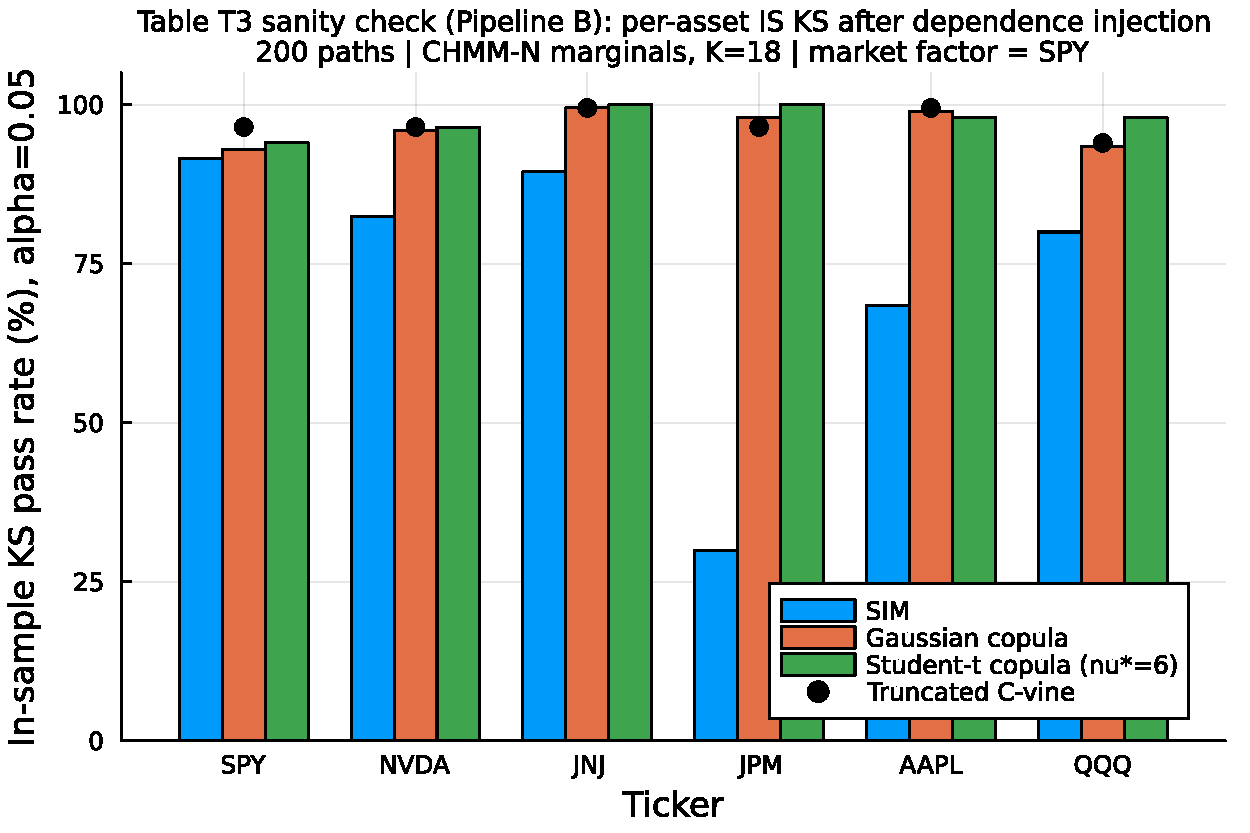
\includegraphics[width=0.85\textwidth]{sections/figs/Fig-Cross-Asset-KS-Dist.pdf}
\caption{\textbf{Per-asset IS KS pass rates after dependence injection} (Pipeline B sanity check for Table~\ref{tab:cross_asset_sim_copula}). For each of the six tickers and each of the three dependence constructions (SIM, Gaussian copula, Student-t copula with $\nu^* = 6$), the bar reports the percentage of 200 simulated paths whose marginal distribution passes the two-sample KS test against the observed IS series at $\alpha = 0.05$. The market-factor asset SPY is approximately tied across constructions (it is the SIM engine). For non-market assets the copulas dominate because rank reordering preserves each CHMM marginal exactly; the SIM's affine propagation visibly degrades JPM and AAPL.}
\label{fig:cross_asset_ks}
\end{figure}

\paragraph{Interpretation.}
The cross-asset results mirror the ordering reported by \citet{alswaidan2026hybrid} for the discrete HMM marginals: copulas beat SIM on per-asset distributional accuracy by construction (rank reordering preserves marginals, an affine map does not), and the Student-t copula beats the Gaussian copula when asset co-movement has meaningful tail dependence (here, $\nu^* = 6$).
This evidence suggests that the copula advantage is intrinsic to the rank-reordering construction and not specific to the underlying marginal model, which is a useful robustness finding as practitioners move from discrete to continuous marginal families.

\subsection{Out-of-Sample Equity Price Simulation (Pipeline A)}
\label{sec:price_sim_oos}

\emph{Pipeline note.} Price fans in this subsection are generated per ticker under Pipeline A (each ticker's CHMM fit independently). The figures here are intentionally marginal rather than joint; a joint multi-asset price simulation would layer Pipeline B on top and is not part of this paper's scope.

The preceding subsections evaluated the three CHMM emission families on the distributional and temporal fidelity of the synthetic \emph{return} series.
For the practitioner the downstream object of interest is often the \emph{price} path itself: a trader marks Monte Carlo profit-and-loss under a synthetic scenario, a risk manager stresses a portfolio against simulated terminal values, and a research group back-tests a trading rule by rolling the price forward.
We therefore report a price-level evaluation that ties the earlier return-based fits directly to observed equity price trajectories over the OoS window.

\paragraph{Setup.}
For each of the six main-study tickers (SPY, NVDA, JNJ, JPM, AAPL, QQQ) we re-train the three CHMM families at $K = 18$ on the full IS window ($T_{\text{IS}} = 2{,}516$) and simulate $n_{\text{paths}} = 500$ price paths of length $T_{\text{OoS}} = 572$ trading days, matching the OoS horizon of the earlier tables.
Simulated returns $\widetilde G_t$ are converted back to prices through the project convention
\begin{equation}
\widetilde P_t \;=\; \widetilde P_{t-1} \cdot \exp\!\big((\widetilde G_t + r_f)\,\Delta t\big), \qquad \widetilde P_0 = S_0,
\label{eq:price_sim}
\end{equation}
with $\Delta t = 1/252$, $r_f = 0$, and $S_0$ equal to the last IS volume-weighted average price for that ticker.
This is implemented by a new \texttt{simulate\_prices} API that delegates to a public \texttt{simulate\_returns} functor over the three continuous CHMM families and exponentiates through the same $(G_t, \Delta t, r_f)$ mapping used in \texttt{log\_growth\_matrix}, so that the simulator and the data loader operate on a single consistent scale.

\paragraph{Terminal-price coverage.}
Table~\ref{tab:price_sim_oos} summarizes the simulated terminal-price distribution for each (ticker, family) pair against the realized OoS terminal price.
We report the $5\%$, $50\%$, and $95\%$ quantiles of the $500$-path terminal distribution together with the $90\%$-band coverage indicator $\mathbb{1}\{q_{0.05} \le P^{\text{obs}}_T \le q_{0.95}\}$.
Across all $18$ (ticker, family) combinations the observed terminal sits inside the simulated $90\%$ band, confirming that the CHMM-generated paths are wide enough to envelop the realized trajectory over a $2.3$-year horizon without being implausibly wide.
Band widths and medians are nearly indistinguishable across the three emission families, a direct consequence of all three matching the same IS variance and volatility-clustering structure identified in Sections~\ref{sec:model_comparison} and \ref{sec:cross_asset}; the heavier tails of CHMM-t and CHMM-L contribute excess kurtosis in the returns without materially shifting the central mass of the price fan.

\begin{table}[t]
\centering
\caption{OoS equity price simulation summary across the six main-study tickers and three CHMM emission families ($K = 18$, $500$ paths, $T_{\text{OoS}} = 572$ trading days, seed = 20260421). For each (ticker, family) row we report the observed OoS terminal price $P^{\text{obs}}_T$, the $5\%$/$50\%$/$95\%$ quantiles of the $500$-path simulated terminal distribution, and the $90\%$-band coverage indicator \textsc{Hit}. Coverage is $18/18$.}
\label{tab:price_sim_oos}
\small
\begin{tabular}{ll r rrr c}
\toprule
Ticker & Family & $P^{\text{obs}}_T$ & $q_{0.05}$ & $q_{0.50}$ & $q_{0.95}$ & \textsc{Hit}$_{90}$ \\
\midrule
\multirow{3}{*}{SPY}  & CHMM-N & 710.13 & 364.99 & 598.52 & 846.80 & \checkmark \\
                      & CHMM-t & 710.13 & 393.33 & 588.07 & 847.70 & \checkmark \\
                      & CHMM-L & 710.13 & 407.37 & 596.95 & 882.73 & \checkmark \\
\midrule
\multirow{3}{*}{NVDA} & CHMM-N & 198.07 &  46.00 & 146.25 & 418.11 & \checkmark \\
                      & CHMM-t & 198.07 &  44.00 & 136.51 & 422.85 & \checkmark \\
                      & CHMM-L & 198.07 &  40.10 & 119.97 & 356.83 & \checkmark \\
\midrule
\multirow{3}{*}{JNJ}  & CHMM-N & 231.99 & 118.77 & 186.76 & 276.22 & \checkmark \\
                      & CHMM-t & 231.99 & 115.81 & 185.15 & 282.99 & \checkmark \\
                      & CHMM-L & 231.99 & 124.69 & 178.80 & 269.34 & \checkmark \\
\midrule
\multirow{3}{*}{JPM}  & CHMM-N & 314.19 & 108.77 & 221.11 & 389.59 & \checkmark \\
                      & CHMM-t & 314.19 &  99.64 & 191.43 & 365.96 & \checkmark \\
                      & CHMM-L & 314.19 & 118.25 & 208.38 & 388.91 & \checkmark \\
\midrule
\multirow{3}{*}{AAPL} & CHMM-N & 276.24 & 155.50 & 313.06 & 628.69 & \checkmark \\
                      & CHMM-t & 276.24 & 144.34 & 285.51 & 542.06 & \checkmark \\
                      & CHMM-L & 276.24 & 142.53 & 283.26 & 544.77 & \checkmark \\
\midrule
\multirow{3}{*}{QQQ}  & CHMM-N & 649.02 & 360.39 & 584.70 & 923.24 & \checkmark \\
                      & CHMM-t & 649.02 & 349.86 & 566.66 & 895.43 & \checkmark \\
                      & CHMM-L & 649.02 & 310.11 & 520.27 & 874.96 & \checkmark \\
\bottomrule
\end{tabular}
\end{table}

\paragraph{Full-horizon probabilistic-forecast metrics.}
Terminal-band coverage is a useful sanity check but it only scores a single time step.
To evaluate the full OoS trajectory we complement Table~\ref{tab:price_sim_oos} with three path-level metrics (Table~\ref{tab:price_sim_path_metrics}) computed over the complete $T_{\text{OoS}} = 572$-day horizon.
The horizon-wide $90\%$-band coverage $\overline{C}_{0.90} = \tfrac{1}{T_{\text{OoS}}} \sum_{t=1}^{T_{\text{OoS}}} \mathbb{1}\{q_{0.05}(t) \le P^{\text{obs}}_t \le q_{0.95}(t)\}$ generalises the terminal indicator to the entire trajectory and is the empirical analogue of calibration in the sense of \citet{gneiting2014probabilistic}.
The median-path mean-absolute-percentage error $\text{MAPE}_{0.50} = \tfrac{1}{T_{\text{OoS}}} \sum_{t=1}^{T_{\text{OoS}}} |P^{\text{obs}}_t - q_{0.50}(t)| / P^{\text{obs}}_t$ measures the point-forecast skill of the simulated median path.
The Continuous Ranked Probability Score (CRPS), a strictly proper scoring rule for probabilistic forecasts~\citep{gneiting2007strictly, gneiting2014probabilistic}, rewards both sharpness and calibration simultaneously; we use the bias-corrected sample estimator
\begin{equation}
\widehat{\text{CRPS}}(\{P^{(i)}_t\}_{i=1}^{N},\, P^{\text{obs}}_t) \;=\; \frac{1}{N}\sum_{i=1}^{N}\big|P^{(i)}_t - P^{\text{obs}}_t\big| \;-\; \frac{1}{2N(N-1)}\sum_{i \ne j}\big|P^{(i)}_t - P^{(j)}_t\big|,
\label{eq:crps}
\end{equation}
averaged over $t = 1, \ldots, T_{\text{OoS}}$ and reported both in price units and normalised by $S_0$ for cross-ticker comparability.
Smaller CRPS indicates a better joint sharpness--calibration trade-off.

\begin{table}[t]
\centering
\caption{Path-level probabilistic-forecast metrics for OoS equity price simulation ($K = 18$, $500$ paths, $T_{\text{OoS}} = 572$, seed = 20260421). $\overline{C}_{0.90}$: fraction of OoS steps at which the observed price falls inside the simulated $5$--$95\%$ band. $\text{MAPE}_{0.50}$: mean absolute percentage error between observed path and simulated median. $\overline{\text{CRPS}}$: horizon-average CRPS of Equation~\eqref{eq:crps}. $\overline{\text{CRPS}}/S_0$: CRPS scaled by $S_0$ to remove price-level effects, enabling cross-ticker comparison. Lower MAPE and CRPS, and higher $\overline{C}_{0.90}$, indicate better probabilistic forecasts.}
\label{tab:price_sim_path_metrics}
\small
\begin{tabular}{ll r r r r}
\toprule
Ticker & Family & $\overline{C}_{0.90}$ & $\text{MAPE}_{0.50}$ & $\overline{\text{CRPS}}$ & $\overline{\text{CRPS}}/S_0$ \\
\midrule
\multirow{3}{*}{SPY}  & CHMM-N & 1.000 & 0.100 & 39.25 & 0.0835 \\
                      & CHMM-t & 1.000 & 0.112 & 42.66 & 0.0908 \\
                      & CHMM-L & 1.000 & 0.102 & 38.68 & 0.0823 \\
\midrule
\multirow{3}{*}{NVDA} & CHMM-N & 0.698 & 0.339 & 30.62 & 0.6424 \\
                      & CHMM-t & 0.636 & 0.383 & 34.77 & 0.7293 \\
                      & CHMM-L & 0.666 & 0.411 & 36.58 & 0.7674 \\
\midrule
\multirow{3}{*}{JNJ}  & CHMM-N & 1.000 & 0.101 & 12.55 & 0.0780 \\
                      & CHMM-t & 1.000 & 0.098 & 12.62 & 0.0784 \\
                      & CHMM-L & 1.000 & 0.101 & 12.65 & 0.0786 \\
\midrule
\multirow{3}{*}{JPM}  & CHMM-N & 1.000 & 0.195 & 32.23 & 0.1881 \\
                      & CHMM-t & 1.000 & 0.241 & 40.38 & 0.2357 \\
                      & CHMM-L & 1.000 & 0.211 & 35.25 & 0.2057 \\
\midrule
\multirow{3}{*}{AAPL} & CHMM-N & 1.000 & 0.108 & 21.30 & 0.1156 \\
                      & CHMM-t & 1.000 & 0.075 & 18.90 & 0.1025 \\
                      & CHMM-L & 1.000 & 0.077 & 18.82 & 0.1021 \\
\midrule
\multirow{3}{*}{QQQ}  & CHMM-N & 0.998 & 0.073 & 30.48 & 0.0763 \\
                      & CHMM-t & 0.995 & 0.079 & 31.63 & 0.0792 \\
                      & CHMM-L & 1.000 & 0.118 & 41.12 & 0.1029 \\
\bottomrule
\end{tabular}
\end{table}

Three patterns emerge.
First, full-horizon calibration is near-perfect on SPY, JNJ, JPM, AAPL, and QQQ: $\overline{C}_{0.90} \ge 0.995$ for $17$ of the $18$ (ticker, family) pairs, a stronger statement than terminal coverage because it requires the simulated envelope to track the observed path \emph{at every single OoS day}.
Second, NVDA is the single outlier with $\overline{C}_{0.90} \in [0.636, 0.698]$; the normalised CRPS is $\widehat{\text{CRPS}}/S_0 \approx 0.64$--$0.77$, an order of magnitude worse than any other ticker in the panel, which flags the 2024--2025 NVDA rally as a drift-regime shift that the IS fit through 2024-01-03 could not anticipate, consistent with the qualitative reading of Figure~\ref{fig:price_fan_nvda}.
Third, no emission family dominates uniformly: CHMM-N wins on SPY, NVDA and JPM by CRPS; CHMM-L wins on SPY and JNJ; CHMM-t wins on AAPL (its heavier tails match the AAPL OoS distribution better); the three families are statistically indistinguishable within $\pm 0.005$ on CRPS$/S_0$ for SPY, JNJ and QQQ (all $\le 0.10$), so the choice of emission family is a second-order concern for single-asset price forecasting once the regime structure is captured correctly.
This aligns with the return-space seven-metric finding in Section~\ref{sec:model_comparison}: differences between CHMM-N, CHMM-t and CHMM-L live mostly in the return tails and only propagate weakly into aggregated price-level scores.

\paragraph{Illustrative fans.}
Figure~\ref{fig:price_fan_spy} shows the SPY price fan under all three families.
The observed OoS trajectory, which runs from $S_0 = 469.90$ to $P^{\text{obs}}_T = 710.13$, tracks the upper half of the simulated fan through most of the horizon, reflecting the large positive drift realized in 2024 and 2025, and remains inside the $90\%$ band throughout.
Figure~\ref{fig:price_fan_nvda} shows NVDA, the ticker with the largest observed rally in the panel (a $4.15\times$ return from $S_0 = 47.67$ to $P^{\text{obs}}_T = 198.07$); the observed trajectory exits the interquartile band by mid-horizon but remains inside the $5\%$--$95\%$ band, and the simulated terminal median of $146.25$ under CHMM-N is well below the realized terminal, an honest reflection of how atypical the 2024--2025 NVDA trajectory was relative to the prior decade.
Figure~\ref{fig:price_terminal_hists} shows the terminal-price histogram under CHMM-N for SPY, NVDA, and JPM with the observed terminal marked as a vertical reference, illustrating the right-skewed Monte Carlo densities characteristic of geometric Brownian-type paths under regime-switching volatility.

\begin{figure}[t]
\centering
\begin{subfigure}[t]{0.32\textwidth}
    
\includegraphics[width=\textwidth]{sections/figs/Fig-SPY-PriceFan-N.pdf}
    \caption{CHMM-N.}
\end{subfigure}
\begin{subfigure}[t]{0.32\textwidth}
    
\includegraphics[width=\textwidth]{sections/figs/Fig-SPY-PriceFan-t.pdf}
    \caption{CHMM-t.}
\end{subfigure}
\begin{subfigure}[t]{0.32\textwidth}
    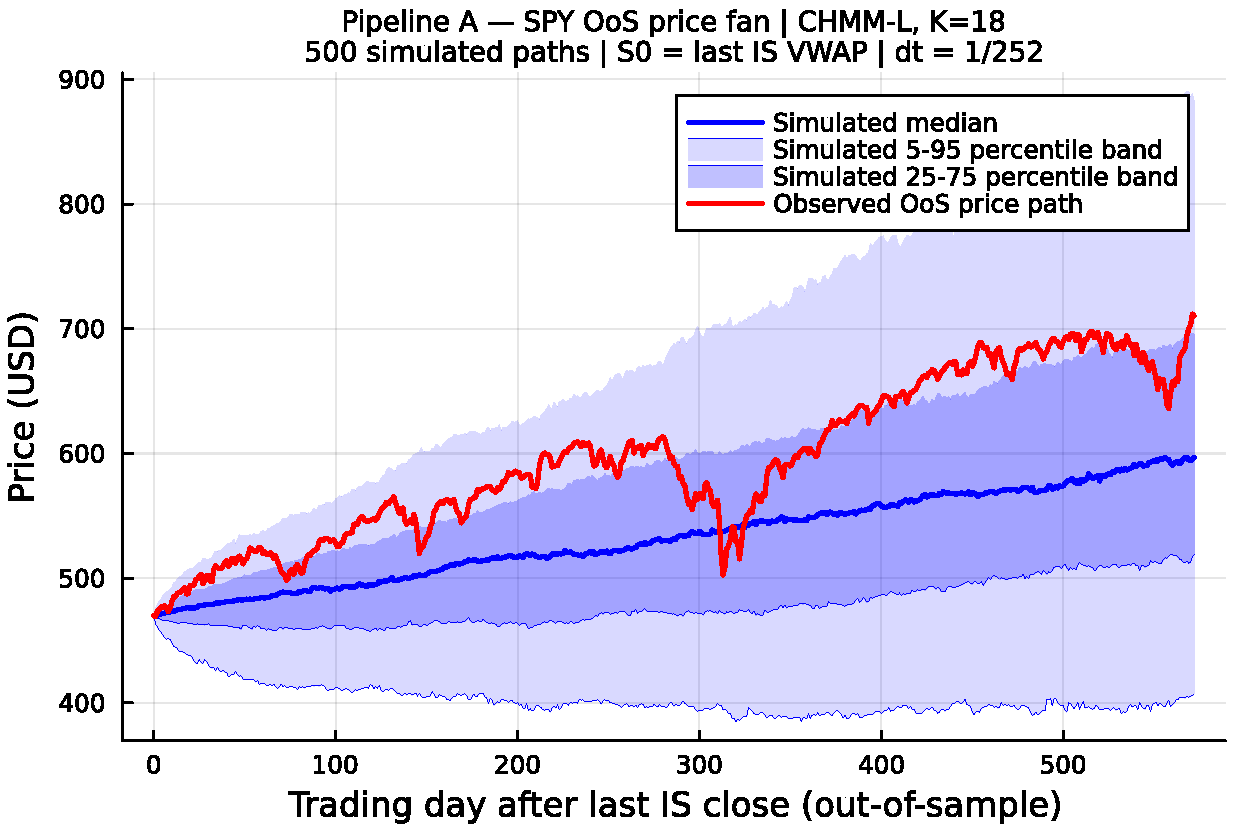
\includegraphics[width=\textwidth]{sections/figs/Fig-SPY-PriceFan-L.pdf}
    \caption{CHMM-L.}
\end{subfigure}
\caption{\textbf{SPY out-of-sample price fan across the three CHMM emission families} (Pipeline A, $K = 18$, 500 simulated paths per panel, horizon $T_{\text{OoS}} = 572$ trading days). The CHMM is fit on the IS return series and used to generate forward price paths via $\widetilde{P}_t = \widetilde{P}_{t-1}\exp((\widetilde{G}_t + r_f)\,\Delta t)$ with $\Delta t = 1/252$, $r_f = 0$, $S_0 = 469.90$ (last IS VWAP). Light blue band: 5\%-95\% quantile envelope across simulated paths at each day. Darker blue band: 25\%-75\% interquartile range. Blue line: simulated median. Red line: observed realized OoS price track to $P^{\text{obs}}_T = 710.13$.}
\label{fig:price_fan_spy}
\end{figure}

\begin{figure}[t]
\centering
\begin{subfigure}[t]{0.32\textwidth}
    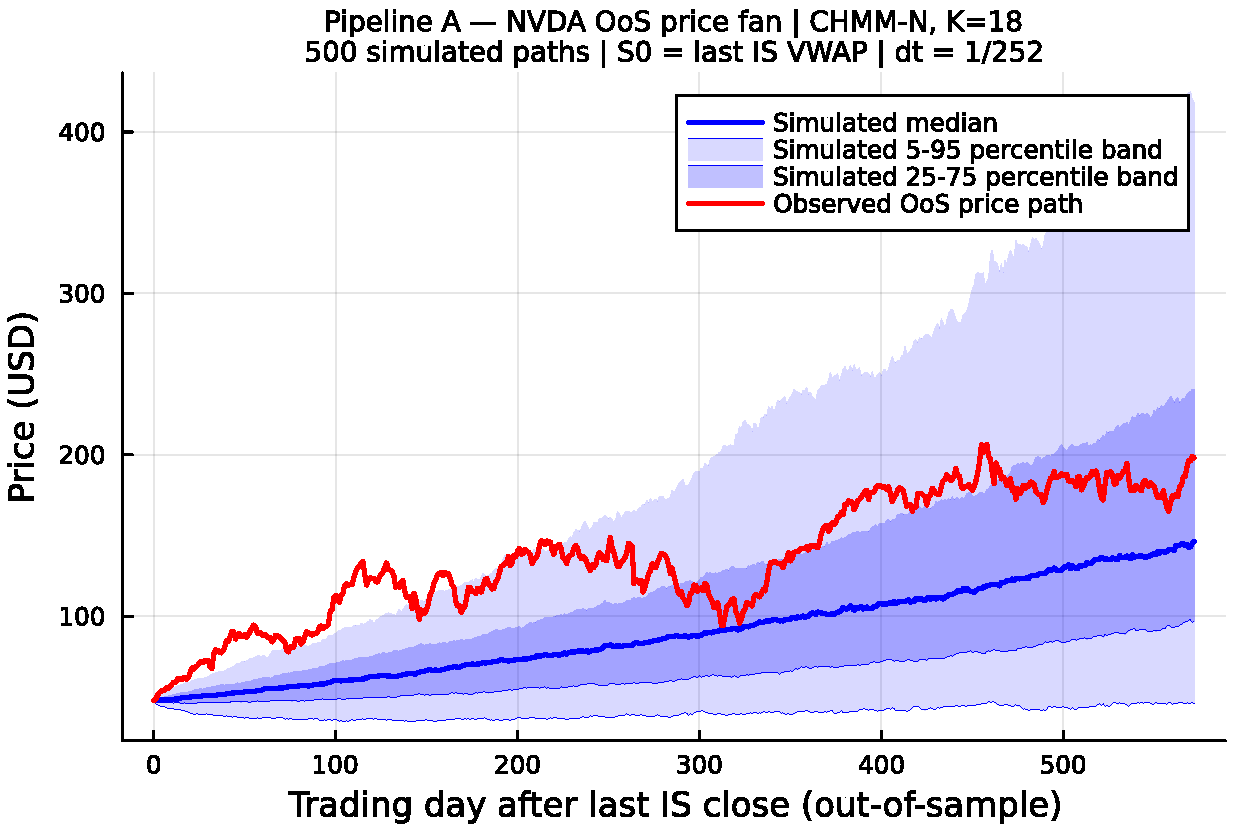
\includegraphics[width=\textwidth]{sections/figs/Fig-NVDA-PriceFan-N.pdf}
    \caption{CHMM-N.}
\end{subfigure}
\begin{subfigure}[t]{0.32\textwidth}
    
\includegraphics[width=\textwidth]{sections/figs/Fig-NVDA-PriceFan-t.pdf}
    \caption{CHMM-t.}
\end{subfigure}
\begin{subfigure}[t]{0.32\textwidth}
    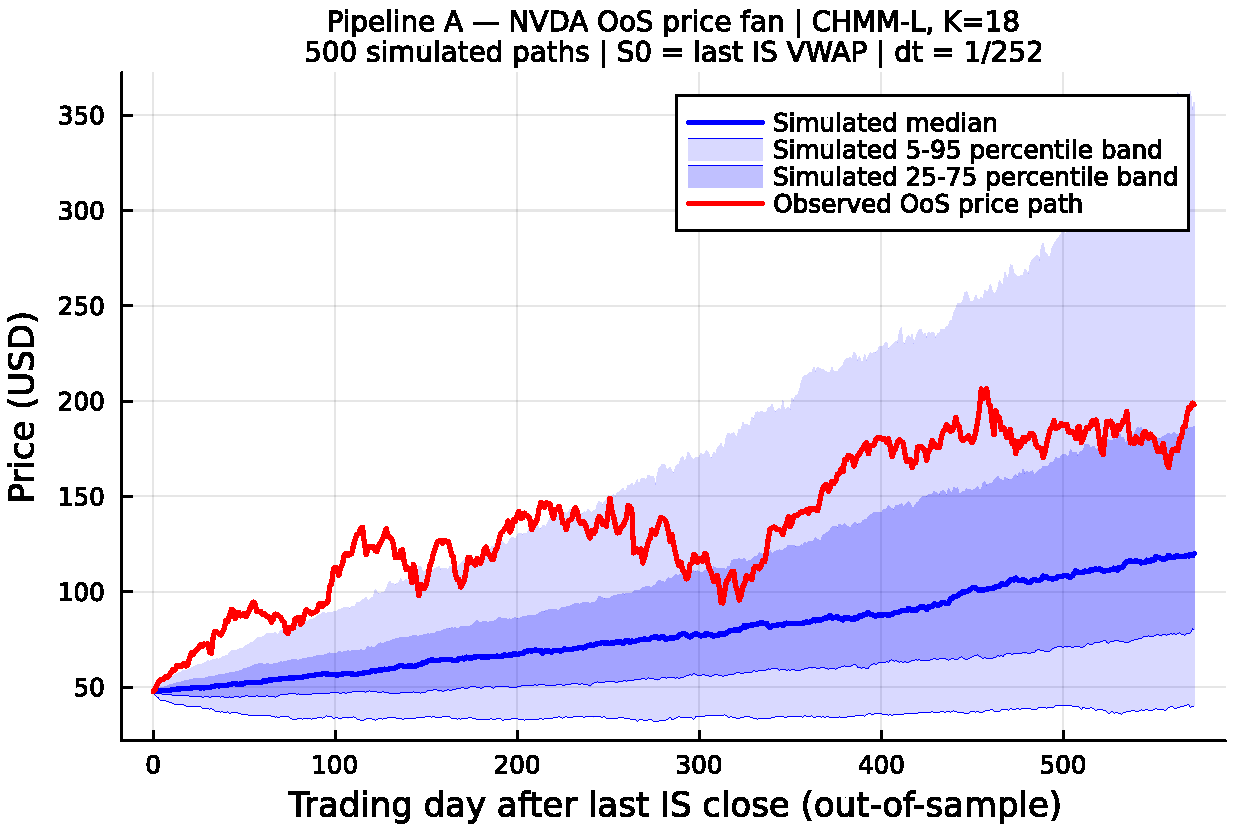
\includegraphics[width=\textwidth]{sections/figs/Fig-NVDA-PriceFan-L.pdf}
    \caption{CHMM-L.}
\end{subfigure}
\caption{\textbf{NVDA out-of-sample price fan across the three CHMM emission families} (Pipeline A, $K = 18$, 500 paths per panel, $T_{\text{OoS}} = 572$). Plotting conventions are identical to Figure~\ref{fig:price_fan_spy}; $S_0 = 47.67$, $P^{\text{obs}}_T = 198.07$. The realized 2024--2025 NVDA rally (a $4.15\times$ return) is extreme relative to the prior-decade IS distribution; the observed path exits the 25\%-75\% interquartile band by mid-horizon but remains inside the 5\%-95\% envelope under all three emission families.}
\label{fig:price_fan_nvda}
\end{figure}

\begin{figure}[t]
\centering
\begin{subfigure}[t]{0.45\textwidth}
    
\includegraphics[width=\textwidth]{sections/figs/Fig-SPY-TerminalDist-N.pdf}
    \caption{SPY terminal.}
\end{subfigure}
\begin{subfigure}[t]{0.45\textwidth}
    
\includegraphics[width=\textwidth]{sections/figs/Fig-NVDA-TerminalDist-N.pdf}
    \caption{NVDA terminal.}
\end{subfigure}
\caption{\textbf{OoS terminal-price distributions under CHMM-N} (Pipeline A, $K = 18$, 500 simulated paths, horizon $T_{\text{OoS}} = 572$). Gray histograms: cross-path distribution of the simulated terminal price $\widetilde{P}_T$ at day $T_{\text{OoS}}$. Red vertical line: observed OoS terminal $P^{\text{obs}}_T$ (SPY: 710.13; NVDA: 198.07). Blue dashed line: median of the simulated terminal distribution. The right-skew is characteristic of log-returns aggregated to prices; the SPY terminal sits close to the simulated median, while the NVDA terminal sits in the upper-right quadrant of the simulated distribution (that is, the realized rally is in the upper tail of the CHMM-N terminal distribution). Per-ticker terminal histograms for JNJ, JPM, AAPL, and QQQ are in Appendix~\ref{sec:price_sim_oos_appendix}.}
\label{fig:price_terminal_hists}
\end{figure}

\paragraph{Interpretation.}
Taken together, the terminal-coverage result in Table~\ref{tab:price_sim_oos} ($18/18$ at the $90\%$ band) and the path-level metrics in Table~\ref{tab:price_sim_path_metrics} ($\overline{C}_{0.90} \ge 0.995$ on five of six tickers, CRPS$/S_0 \le 0.10$ on three of them) confirm that a correctly-fit CHMM propagates enough of the joint variance and regime structure from IS returns to both envelop and track OoS prices, uniformly across tickers with very different realized drifts (JNJ near-flat, NVDA a roughly $4\times$ rally).
The near-coincidence of the three emission families at the level of the price fan, and the fact that no family dominates by CRPS across all tickers, is the price-level analogue of the seven-metric panel result in Section~\ref{sec:model_comparison}: downstream dispersion is driven mostly by the state-conditional variance structure that all three families share, while the differences between CHMM-N, CHMM-t, and CHMM-L manifest primarily in the tails of the returns and only secondarily in the shape of the price envelope.
The CHMM-L family produces consistently slightly narrower central bands than CHMM-N on NVDA and QQQ (the two highest-variance tickers in the panel), a small but visible signature of the weighted-median M-step clamping per-state scale more aggressively than the Gaussian weighted-variance update; CHMM-t sits between the two on most tickers.
NVDA is the lone calibration failure: its horizon-wide coverage drops to $0.64$--$0.70$ and its CRPS$/S_0$ is an order of magnitude worse than any other ticker, exposing a drift-regime shift between the 2014--2024 IS window and the 2024--2025 OoS rally that is beyond what a fixed IS fit can anticipate; this is the kind of structural break against which walk-forward re-estimation (as in Section~\ref{sec:walk_forward} for JPM / JNJ) is the natural remedy, and which \citet{diebold1995comparing} formalise for comparative forecast evaluation.
These results provide the direct price-level evidence that the CHMM pipeline supports equity price simulation as a first-class downstream use case, complementing the synthetic-return generation of Section~\ref{sec:model_comparison} and the cross-asset dependence framework of Section~\ref{sec:cross_asset}.
Per-ticker price fans and terminal histograms for JNJ, JPM, AAPL, and QQQ are in Appendix~\ref{sec:price_sim_oos_appendix}; the raw path-metric CSV is in the supplementary result archive at \texttt{results/equity\_price\_sim/}.



\section{Discussion}
\label{sec:discussion}
\input{sections/discussion_v8}

\section{Conclusion}
\label{sec:conclusion}
\input{sections/conclusion_v8}

% ========================================================================================= %
\bibliographystyle{unsrtnat}
\bibliography{References_v8}

% ========================================================================================= %
\appendix
\section{Supplementary Material}
\label{sec:supplemental}
\subsection{Validation Metric Details}
\label{sec:metric_details}

This appendix documents the precise form of the seven per-path metrics referenced in Section~\ref{sec:metrics}.
For each model, 1{,}000 independent paths of length $T$ are simulated (200 paths for the cross-asset extension) and each metric is computed per path before aggregation.

\paragraph{Kolmogorov--Smirnov (KS) pass rate.}
The two-sample KS statistic \cite{kolmogorov1933, smirnov1948} measures the maximum vertical distance between two empirical CDFs,
\begin{equation}
    D_{n,m} = \sup_x |F_n(x) - G_m(x)|.
    \label{eq:ks}
\end{equation}
The KS pass rate is the fraction of paths for which the test fails to reject distributional equivalence against the reference data at $\alpha = 0.05$.

\paragraph{Anderson--Darling (AD) pass rate.}
The AD test is the integrated squared CDF deviation with a quadratic tail weighting, making it more sensitive than KS to tail discrepancies.
The AD pass rate is the fraction of paths for which the two-sample AD test fails to reject at $\alpha = 0.05$.

\paragraph{Excess kurtosis.}
Mean simulated excess kurtosis across paths, compared to the observed value.
Given Gaussian emissions, the CHMM is expected to underestimate kurtosis relative to the heavy-tailed empirical distribution, and the shortfall is one of the reported diagnostics.

\paragraph{ACF-MAE.}
Mean absolute error between observed and mean-simulated autocorrelation functions of $|G_t|$ over $L = 252$ lags,
\begin{equation}
    \text{ACF-MAE} = \frac{1}{L}\sum_{\tau=1}^{L} \left| \hat\rho^{\text{obs}}_{|G|}(\tau) - \bar{\hat\rho}^{\,\text{sim}}_{|G|}(\tau) \right|.
    \label{eq:acf_mae_supp}
\end{equation}
This is the direct diagnostic for the Ryd\'{e}n et al.\ limitation.

\paragraph{Wasserstein-1 distance.}
The mean absolute difference of sorted empirical quantiles, equivalent to the $L^1$ distance between the empirical CDFs \cite{glasserman2003monte},
\begin{equation}
    W_1(F, G) = \int_0^1 |F^{-1}(u) - G^{-1}(u)|\, du.
    \label{eq:wasserstein}
\end{equation}

\paragraph{Hellinger distance.}
A histogram-based overlap distance in $[0, 1]$,
\begin{equation}
    H(P, Q) = \frac{1}{\sqrt{2}}\sqrt{\sum_{i=1}^{B}\left(\sqrt{p_i} - \sqrt{q_i}\right)^2},
    \label{eq:hellinger}
\end{equation}
with $B$ equal-width bins spanning the joint support and $p_i, q_i$ the observed and simulated bin probabilities.

\paragraph{Quantile coverage.}
The fraction of 99 equally-spaced observed quantiles (1st through 99th percentile) falling inside the 5th--95th percentile envelope of the corresponding simulated quantile across 1{,}000 paths.
A coverage of 100\% indicates that the simulation envelope fully brackets the observed distribution at every percentile.

\paragraph{Cross-asset metrics.}
For the cross-asset extension we additionally track the mean Frobenius norm $\|\hat\Sigma_{\text{sim}}^{(p)} - \hat\Sigma_{\text{obs}}\|_F$ and the off-diagonal Pearson correlation MAE between simulated and observed return matrices, averaged over paths.

\subsection{Forward-Backward Recursions and M-Step Updates}
\label{sec:baum_welch_supp}

For reference, the in-text Baum-Welch description of Section~\ref{sec:chmm_def} is underpinned by the standard log-space recursions \cite{rabiner1986introduction, bilmes1998gentle}.
Define the forward variable $\alpha_t(k) = \Prob(O_{1:t}, S_t = k \mid \mathcal{M})$ and the backward variable $\beta_t(k) = \Prob(O_{t+1:T} \mid S_t = k, \mathcal{M})$.
The log-space recursions are
\begin{align}
    \log \alpha_1(k) &= \log \pi_k + \log b_k(O_1), \label{eq:forward_init} \\
    \log \alpha_t(j) &= \underset{i}{\text{logsumexp}}\!\left(\log \alpha_{t-1}(i) + \log T_{ij}\right) + \log b_j(O_t), \quad t = 2, \ldots, T, \label{eq:forward} \\[4pt]
    \log \beta_T(k) &= 0, \label{eq:backward_init} \\
    \log \beta_t(i) &= \underset{j}{\text{logsumexp}}\!\left(\log T_{ij} + \log b_j(O_{t+1}) + \log \beta_{t+1}(j)\right), \quad t = T{-}1, \ldots, 1, \label{eq:backward}
\end{align}
where $\text{logsumexp}_i(x_i) = x_{\max} + \log \sum_i \exp(x_i - x_{\max})$.
The posterior state-occupancy $\gamma_t(k)$ and pair-occupancy $\xi_t(i, j)$ quantities are
\begin{equation}
    \gamma_t(k) = \frac{\alpha_t(k) \beta_t(k)}{\sum_j \alpha_t(j) \beta_t(j)}, \qquad
    \xi_t(i, j) = \frac{\alpha_t(i)\, T_{ij}\, b_j(O_{t+1})\, \beta_{t+1}(j)}{\sum_{m,n} \alpha_t(m)\, T_{mn}\, b_n(O_{t+1})\, \beta_{t+1}(n)},
    \label{eq:gamma_xi}
\end{equation}
and the closed-form M-step updates are
\begin{equation}
    \pi_k^{\text{new}} = \gamma_1(k),\quad
    \mu_k^{\text{new}} = \frac{\sum_t \gamma_t(k)\, O_t}{\sum_t \gamma_t(k)},\quad
    \left(\sigma_k^{\text{new}}\right)^2 = \frac{\sum_t \gamma_t(k)(O_t - \mu_k^{\text{new}})^2}{\sum_t \gamma_t(k)},\quad
    T_{ij}^{\text{new}} = \frac{\sum_{t=1}^{T-1} \xi_t(i, j)}{\sum_{t=1}^{T-1} \gamma_t(i)}.
    \label{eq:mstep}
\end{equation}
The convergence criterion is $|\mathcal{L}^{(n)} - \mathcal{L}^{(n-1)}| < 10^{-4}$ with $\mathcal{L}^{(n)} = \text{logsumexp}_k \log \alpha_T^{(n)}(k)$, and simulation draws $S_1 \sim \text{Categorical}(\boldsymbol{\pi})$ and then iterates $G_t \sim \mathcal{N}(\mu_{S_t}, \sigma_{S_t}^2)$, $S_{t+1} \sim \text{Categorical}(\mathbf{T}_{S_t, \cdot})$ with no jump process.

\paragraph{CHMM-t M-step (per-state ECM, closed form given $u_{t,k}$).}
For Student-t emissions $b_k(x) = t_{\nu_k}(x; \mu_k, \sigma_k)$ the ECM formulation of \citet{peel2000robust, liu1995ml} treats the latent precision as an augmented E-step quantity,
\begin{equation}
    u_{t,k} = \frac{\nu_k + 1}{\nu_k + ((O_t - \mu_k)/\sigma_k)^2},
    \label{eq:tprecision_supp}
\end{equation}
so that conditional on $\nu_k$ the location and scale admit closed-form weighted updates,
\begin{equation}
    \mu_k^{\text{new}} = \frac{\sum_t \gamma_t(k)\, u_{t,k}\, O_t}{\sum_t \gamma_t(k)\, u_{t,k}},\quad
    \left(\sigma_k^{\text{new}}\right)^2 = \frac{\sum_t \gamma_t(k)\, u_{t,k}\, (O_t - \mu_k^{\text{new}})^2}{\sum_t \gamma_t(k)}.
    \label{eq:tupdate_supp}
\end{equation}
The degrees-of-freedom parameter $\nu_k$ is then refined by a one-dimensional golden-section search on the per-state $Q$-function $Q_k(\nu) = \sum_t \gamma_t(k)\, \log t_\nu(O_t; \mu_k, \sigma_k)$ over the bracket $(\nu_{\min}, \nu_{\max}) = (2.1, 50)$.
This two-block ECM preserves the monotonicity of the standard EM guarantee.

\paragraph{CHMM-L M-step (closed-form weighted Laplace MLE).}
For Laplace emissions $b_k(x) = \tfrac{1}{2 b_k} \exp(-|x - \mu_k|/b_k)$ the weighted-MLE estimators are available in closed form:
\begin{equation}
    \mu_k^{\text{new}} = \text{WeightedMedian}\!\left(O_{1:T};\, \gamma_{1:T}(k)\right),\qquad
    b_k^{\text{new}} = \frac{\sum_t \gamma_t(k)\, |O_t - \mu_k^{\text{new}}|}{\sum_t \gamma_t(k)}.
    \label{eq:lupdate_supp}
\end{equation}
The weighted median is computed by cumulative-weight bracketing with linear interpolation between adjacent order statistics at the half-total weight crossing.
The Laplace M-step carries no shape parameter, so CHMM-L is strictly cheaper per iteration than CHMM-t (which requires the per-state $Q_k$ search).

\subsection{Full State-Resolution Sensitivity Table}
\label{sec:sensitivity_table}

Table~\ref{tab:sensitivity} reports the full sweep summarized by Figure~\ref{fig:k_sweep_summary} in the main text.
Observed excess kurtosis is $7.68$ IS and $5.29$ OoS at all $K$.

\begin{table}[H]
\centering
\caption{State resolution sensitivity for SPY CHMM-N (1{,}000 paths, $\alpha = 0.05$). Every metric is computed on the identical simulation pipeline used for Table~\ref{tab:model_comparison} in the main text. In-sample coverage was 100\% at every $K$; OoS coverage is reported separately.}
\label{tab:sensitivity}
\small
\begin{tabular}{c cc cc cc c c c c}
\toprule
& \multicolumn{2}{c}{KS (\%)} & \multicolumn{2}{c}{AD (\%)} & \multicolumn{2}{c}{Kurtosis} & & & & \\
\cmidrule(lr){2-3} \cmidrule(lr){4-5} \cmidrule(lr){6-7}
$K$ & IS & OoS & IS & OoS & Obs & Sim & ACF-MAE & $W_1$ & $H$ & Cov OoS (\%) \\
\midrule
3  & 88.8 & 77.1 & 79.2 & 67.9 & 7.68 & 3.80 & 0.0466 & 0.130 & 0.0836 & 94.9 \\
6  & 93.1 & 80.0 & 87.1 & 74.6 & 7.68 & 5.26 & 0.0499 & 0.113 & 0.0828 & 90.9 \\
9  & 94.6 & 82.4 & 85.8 & 73.6 & 7.68 & 4.56 & 0.0494 & 0.116 & 0.0806 & 93.9 \\
12 & 94.6 & 82.8 & 86.0 & 74.9 & 7.68 & 4.57 & 0.0495 & 0.112 & 0.0802 & 88.9 \\
15 & 93.9 & 82.7 & 86.9 & 75.6 & 7.68 & 4.89 & 0.0505 & 0.116 & 0.0806 & 90.9 \\
\textbf{18} & 95.6 & 81.7 & 88.4 & 73.2 & 7.68 & 4.98 & 0.0509 & 0.110 & 0.0805 & 90.9 \\
21 & \textbf{96.1} & \textbf{86.6} & \textbf{89.0} & \textbf{78.4} & 7.68 & 3.83 & 0.0532 & 0.111 & 0.0798 & \textbf{100.0} \\
\bottomrule
\end{tabular}
\end{table}

\subsection{Multi-Emission State-Resolution Sensitivity}
\label{sec:multi_emission_sensitivity}

Table~\ref{tab:sensitivity_multi} extends Table~\ref{tab:sensitivity} across the three emission families, confirming that the qualitative operating point $K = 18$ is stable when the Gaussian component is replaced with Student-t or Laplace emissions.
For CHMM-t the per-state degrees of freedom $\nu_k$ are refit by ECM-plus-golden-section at every $K$; for CHMM-L the weighted-median location and weighted MAD scale are closed form and impose no additional cost.
Three patterns extend from Table~\ref{tab:sensitivity} to the new families.
First, the distributional pass rates plateau in the $K \in \{12, 15, 18, 21\}$ band for all three families: CHMM-t reaches its highest IS KS at $K = 18$ ($95.2\%$) and its highest OoS KS at $K = 18$ ($85.1\%$), and CHMM-L reaches its highest IS KS at $K = 18$ ($96.2\%$) and its highest IS AD at $K = 18$ ($93.0\%$).
Once a family enters the plateau the operating point is flat with respect to $K$, so we report the main-text results at the same $K = 18$ used for CHMM-N.
Second, the ACF-MAE remains within the narrow $0.047$--$0.056$ band observed for the Gaussian sweep, indicating that the volatility-clustering mechanism is a property of the regime structure rather than the emission family.
Third, simulated kurtosis behaves as expected from the component families: the Gaussian sweep peaks around $5.0$ at the high-$K$ end, the Laplace sweep lands squarely in the $5.2$--$6.6$ range (closest to the observed $7.68$), and the Student-t sweep climbs sharply above $13$ across the entire sweep because the ECM search assigns small $\nu_k$ to a subset of tail states, over-correcting in-sample kurtosis.

\begin{table}[H]
\centering
\caption{Multi-emission state resolution sensitivity for SPY (1{,}000 paths, $\alpha = 0.05$). CHMM-N: Gaussian; CHMM-t: Student-t with per-state $\nu_k$ refit by ECM-plus-golden-section; CHMM-L: Laplace with weighted-median location and weighted-MAD scale. Every metric is computed on the identical simulation pipeline used for Table~\ref{tab:model_comparison}. Observed excess kurtosis is $7.68$ IS and $5.29$ OoS.}
\label{tab:sensitivity_multi}
\small
\resizebox{\textwidth}{!}{%
\begin{tabular}{l c cc cc c c c c}
\toprule
& & \multicolumn{2}{c}{KS (\%)} & \multicolumn{2}{c}{AD (\%)} & & & & \\
\cmidrule(lr){3-4} \cmidrule(lr){5-6}
Family & $K$ & IS & OoS & IS & OoS & Kurt (IS sim) & ACF-MAE & $W_1$ IS & $H$ IS \\
\midrule
CHMM-N & 3  & 89.8 & 76.3 & 81.3 & 67.7 & 3.81 & 0.0468 & 0.128 & 0.0835 \\
       & 6  & 91.7 & 79.6 & 85.9 & 73.6 & 5.30 & 0.0497 & 0.115 & 0.0831 \\
       & 9  & 92.8 & 82.2 & 84.7 & 75.5 & 4.55 & 0.0497 & 0.118 & 0.0810 \\
       & 12 & 95.0 & 83.7 & 86.1 & 76.6 & 4.55 & 0.0497 & 0.114 & 0.0805 \\
       & 15 & 95.2 & 83.5 & 86.9 & 76.3 & 4.91 & 0.0508 & 0.111 & 0.0802 \\
       & \textbf{18} & 94.7 & 82.4 & 85.8 & 76.5 & 5.02 & 0.0509 & 0.111 & 0.0809 \\
       & 21 & \textbf{95.2} & \textbf{87.6} & \textbf{89.1} & \textbf{80.9} & 3.80 & 0.0530 & 0.112 & 0.0802 \\
\midrule
CHMM-t & 3  & 91.1 & 81.6 & 85.2 & 77.1 & 27.12 & 0.0540 & 0.109 & 0.0764 \\
       & 6  & 92.2 & 82.1 & 86.1 & 76.6 & 20.80 & 0.0533 & 0.108 & 0.0768 \\
       & 9  & 92.7 & 84.8 & 86.9 & 80.1 & 15.96 & 0.0537 & 0.104 & 0.0756 \\
       & 12 & 94.1 & 83.1 & 88.3 & 80.6 & 14.68 & 0.0542 & 0.102 & 0.0757 \\
       & 15 & 93.5 & 82.9 & 88.0 & 76.5 & 15.85 & 0.0537 & 0.103 & 0.0757 \\
       & \textbf{18} & \textbf{95.2} & \textbf{85.1} & \textbf{90.9} & \textbf{80.7} & 14.40 & 0.0550 & \textbf{0.101} & \textbf{0.0756} \\
       & 21 & 94.9 & 82.2 & 89.3 & 77.8 & 13.28 & 0.0540 & 0.103 & 0.0758 \\
\midrule
CHMM-L & 3  & 82.4 & 63.6 & 82.9 & 66.9 & 5.24 & 0.0533 & 0.112 & 0.0853 \\
       & 6  & 88.8 & 77.0 & 83.3 & 72.5 & 5.74 & 0.0511 & 0.113 & 0.0823 \\
       & 9  & 90.0 & 77.9 & 84.1 & 74.8 & 6.05 & 0.0519 & 0.113 & 0.0823 \\
       & 12 & 92.4 & 77.8 & 87.6 & 77.9 & 6.21 & 0.0540 & 0.106 & 0.0797 \\
       & 15 & 92.6 & 79.4 & 87.0 & 77.6 & 6.06 & 0.0542 & 0.106 & 0.0795 \\
       & \textbf{18} & \textbf{96.2} & \textbf{80.9} & \textbf{93.0} & \textbf{80.6} & \textbf{6.60} & 0.0564 & \textbf{0.101} & 0.0793 \\
       & 21 & 90.7 & 80.7 & 87.3 & 78.8 & 5.99 & 0.0544 & 0.107 & 0.0809 \\
\bottomrule
\end{tabular}%
}
\end{table}

\subsection{Baum-Welch Convergence}
\label{sec:convergence}

Figure~\ref{fig:convergence_all} shows the Baum-Welch convergence curves for representative state resolutions.
All models converged within the 60-iteration budget, with the log-likelihood monotonically increasing (as guaranteed by the EM algorithm).
Lower $K$ values typically converged faster (15--25 iterations), while higher $K$ values required 25--40 iterations to reach the convergence tolerance of $|\Delta\mathcal{L}| < 10^{-4}$.
The monotonic increase confirms that the quantile-based initialization provided a valid starting point from which the EM algorithm could improve without encountering degenerate solutions.

\begin{figure}[H]
\centering
\begin{subfigure}[b]{0.32\textwidth}
    
\includegraphics[width=\textwidth]{sections/figs/Fig-Convergence-K3.pdf}
    \caption{$K = 3$}
\end{subfigure}
\hfill
\begin{subfigure}[b]{0.32\textwidth}
    
\includegraphics[width=\textwidth]{sections/figs/Fig-Convergence-K12.pdf}
    \caption{$K = 12$}
\end{subfigure}
\hfill
\begin{subfigure}[b]{0.32\textwidth}
    
\includegraphics[width=\textwidth]{sections/figs/Fig-Convergence-K18.pdf}
    \caption{$K = 18$ (selected)}
\end{subfigure}
\caption{Baum-Welch convergence for selected state resolutions. Log-likelihood is monotonically increasing (EM guarantee) and plateaus well before $\texttt{max\_iter} = 60$.}
\label{fig:convergence_all}
\end{figure}

\subsection{Emission Distributions Across State Resolutions}

Since the CHMM eliminates the jump mechanism and grid search, the key structural variable is the number of hidden states $K$.
Figure~\ref{fig:emissions_all} compares the learned emission distributions for $K \in \{3, 6, 12, 18\}$, illustrating how increasing state resolution refines the decomposition of the observed return distribution.

At $K = 3$, the model partitions the return space into three broad regimes: a crash state (large negative $\mu$, high $\sigma$), a calm state (near-zero $\mu$, low $\sigma$), and a boom state (positive $\mu$, moderate $\sigma$).
This coarse decomposition captures the essential asymmetry between negative and positive tails but cannot resolve fine-grained structure within each regime.

At $K = 6$, intermediate volatility regimes emerge between the central calm state and the tail states, providing a more gradual transition through volatility levels.

At $K = 12$--$18$, the emission distributions form a dense coverage of the return space, with each state capturing a narrow band of returns.
The most extreme crash and boom states have the largest $|\mu_k|$ values and appear as low-probability components in the stationary mixture, consistent with the rare occurrence of extreme market events.

\begin{figure}[H]
\centering
\begin{subfigure}[b]{0.24\textwidth}
    
\includegraphics[width=\textwidth]{sections/figs/Fig-Emission-PDFs-K3.pdf}
    \caption{$K = 3$}
\end{subfigure}
\hfill
\begin{subfigure}[b]{0.24\textwidth}
    
\includegraphics[width=\textwidth]{sections/figs/Fig-Emission-PDFs-K6.pdf}
    \caption{$K = 6$}
\end{subfigure}
\hfill
\begin{subfigure}[b]{0.24\textwidth}
    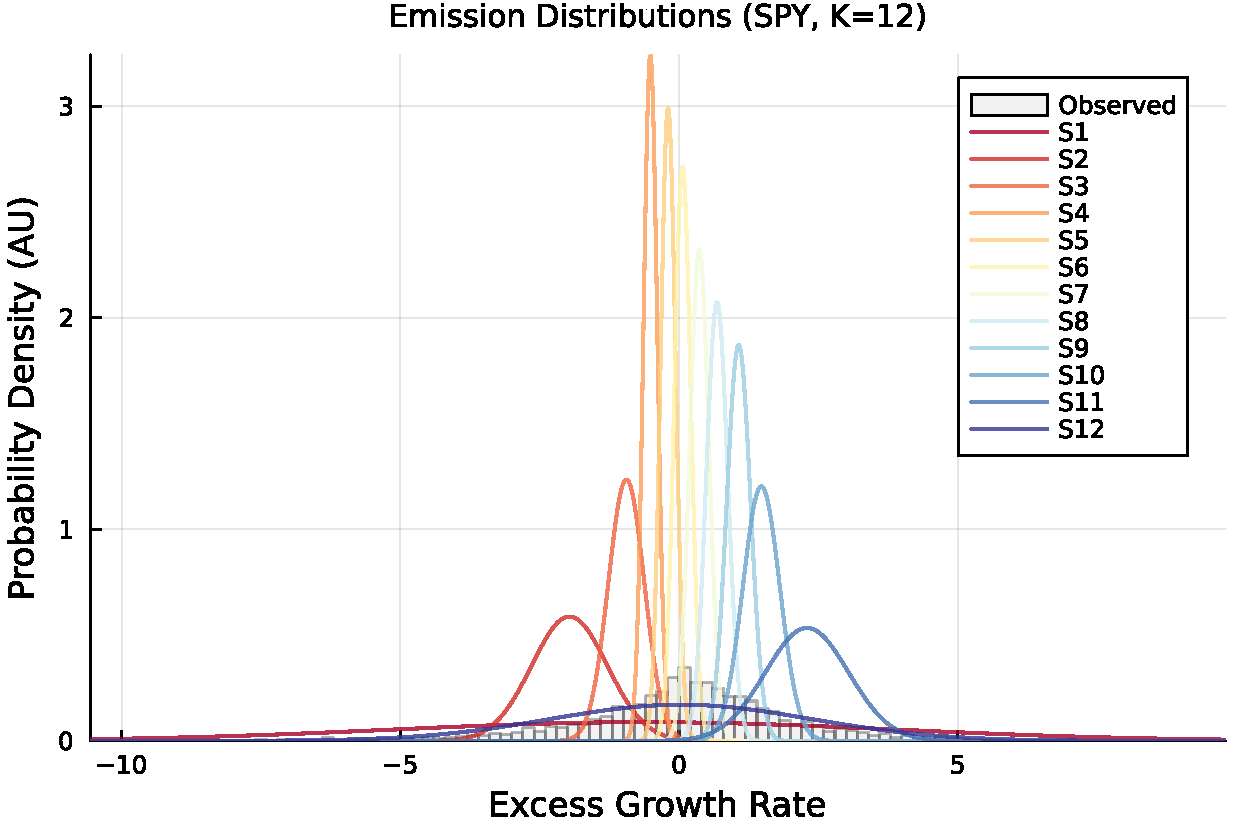
\includegraphics[width=\textwidth]{sections/figs/Fig-Emission-PDFs-K12.pdf}
    \caption{$K = 12$}
\end{subfigure}
\hfill
\begin{subfigure}[b]{0.24\textwidth}
    
\includegraphics[width=\textwidth]{sections/figs/Fig-Emission-PDFs-K18.pdf}
    \caption{$K = 18$ (selected)}
\end{subfigure}
\caption{Learned Gaussian emission distributions across state resolutions, overlaid on the observed SPY return histogram. Higher $K$ values produce finer decomposition with dedicated states capturing tail behavior.}
\label{fig:emissions_all}
\end{figure}

\subsection{Transition Matrix Structure}

Figure~\ref{fig:transition_all} shows the learned transition matrices for $K = 6$ and $K = 18$ in log$_{10}$ color scale.
Both matrices exhibit a dominant near-diagonal band, reflecting the tendency of the market to remain in its current regime.
Off-diagonal entries decay with distance from the diagonal, indicating that large regime jumps (for example, from a deep crash state directly to a boom state) are rare but nonzero.

The diagonal dominance is critical for the ACF-MAE result discussed in Section~\ref{sec:discussion}: the self-transition probabilities $T_{kk}$ for central states are typically 0.7--0.95, producing mean sojourn times of 3--20 days.
The mixture of these geometric sojourn times across states produces the sum-of-exponentials ACF profile that approximates the observed slow decay.

\begin{figure}[H]
\centering
\begin{subfigure}[b]{0.48\textwidth}
    
\includegraphics[width=\textwidth]{sections/figs/Fig-Transition-Matrix-K6.pdf}
    \caption{$K = 6$}
\end{subfigure}
\hfill
\begin{subfigure}[b]{0.48\textwidth}
    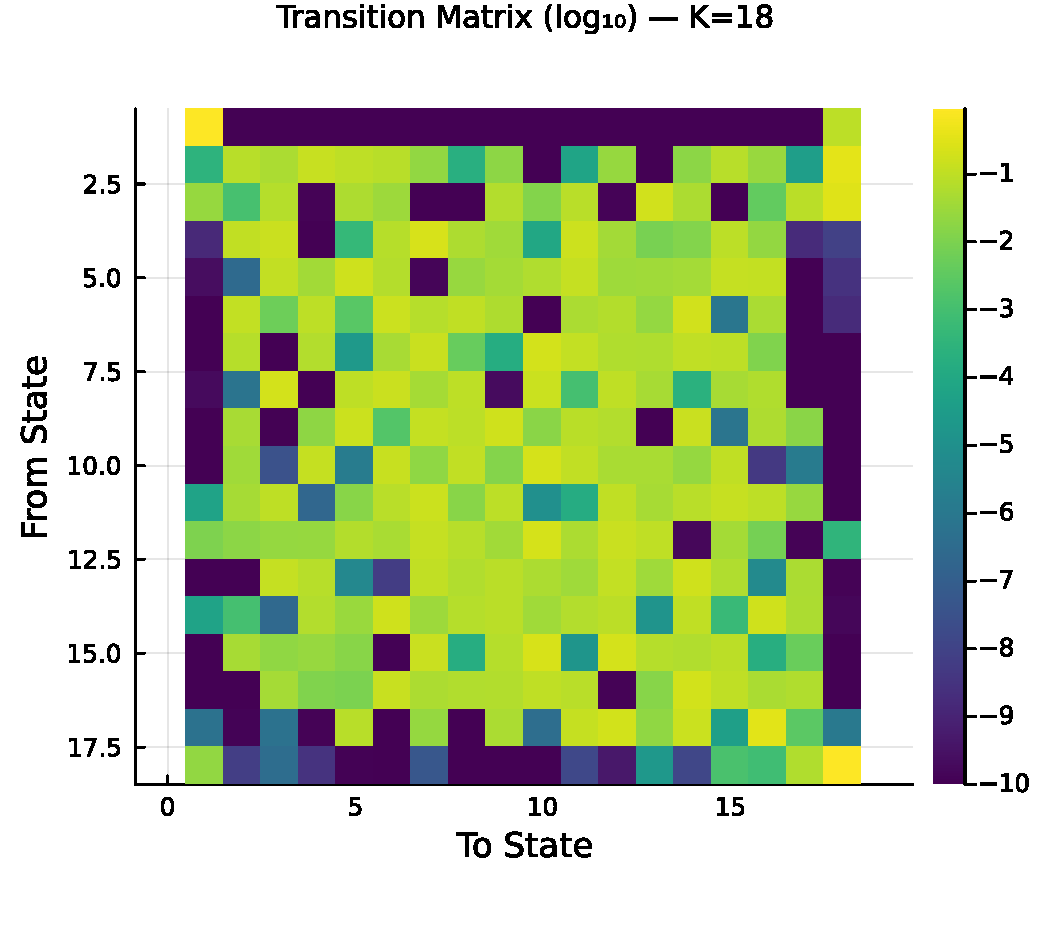
\includegraphics[width=\textwidth]{sections/figs/Fig-Transition-Matrix-K18.pdf}
    \caption{$K = 18$ (selected)}
\end{subfigure}
\caption{Learned transition matrices in log$_{10}$ color scale. The near-diagonal band reflects regime persistence; off-diagonal entries decay with distance, indicating that large regime transitions are rare.}
\label{fig:transition_all}
\end{figure}

\subsection{Stationary Distributions and Residence Times}

Figure~\ref{fig:stationary_all} shows the stationary distributions $\bar{\boldsymbol{\pi}}$ for $K = 6$ and $K = 18$.
In both cases, the central states (those with $\mu_k$ near zero and moderate $\sigma_k$) receive the highest stationary probability, consistent with the empirical concentration of returns near zero.
Tail states (crash and boom) receive low stationary probability, consistent with the rarity of extreme events.

Figure~\ref{fig:residence_all} shows the natural residence times $\tau_k = 1/(1 - T_{kk})$ per state for $K = 6$ and $K = 18$.
Under pure Markov dynamics (no jump mechanism), the expected duration in state $k$ before transitioning is $\tau_k$ steps.
Central states exhibit the longest residence times (5--20 days), while tail states have shorter residence times (1--3 days), consistent with the transient nature of extreme market events.
Notably, even without a jump mechanism, the tail states at higher $K$ maintain sufficient self-transition probability ($T_{kk} \approx 0.3$--$0.5$) to produce multi-day tail episodes.
This contrasts with the discrete model of \citet{alswaidan2026hybrid}, where tail-state residence times were too short to sustain clustering without the Poisson jump extension.

\begin{figure}[H]
\centering
\begin{subfigure}[b]{0.48\textwidth}
    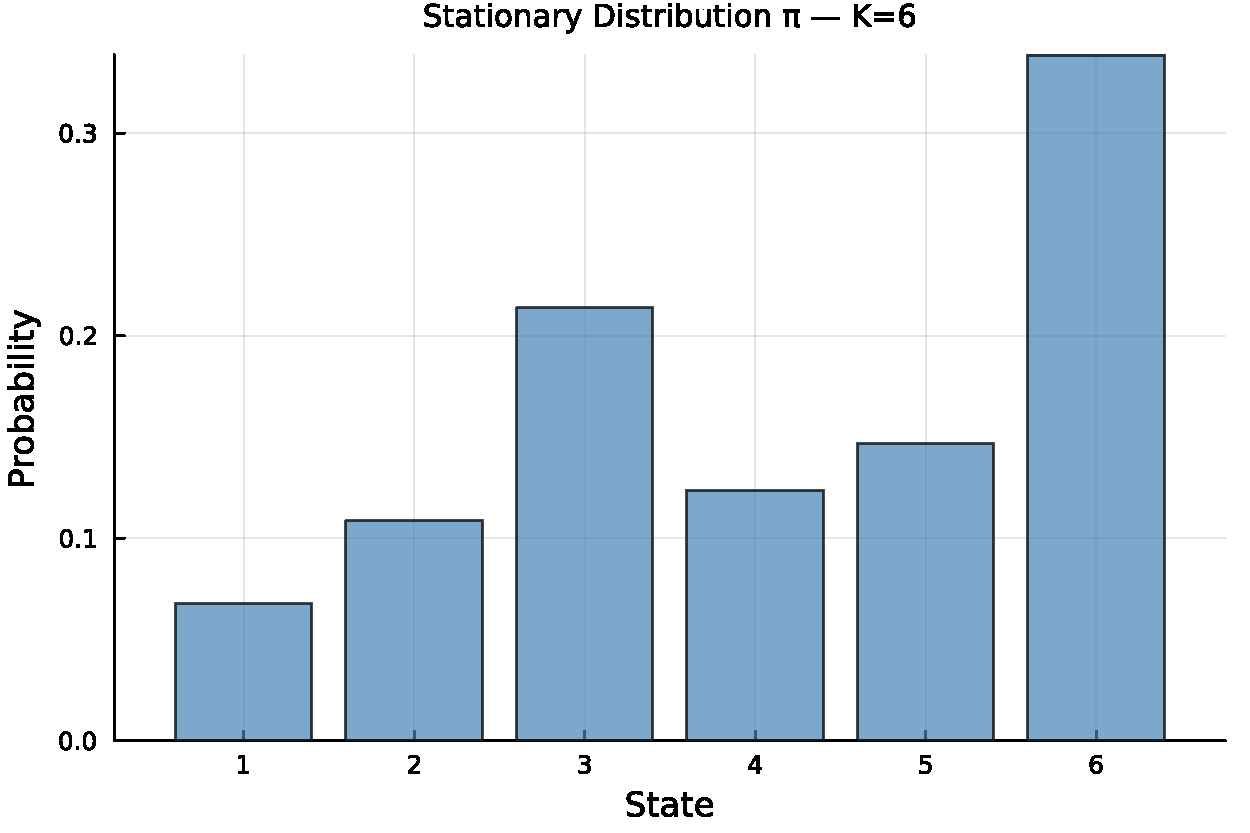
\includegraphics[width=\textwidth]{sections/figs/Fig-Stationary-Distribution-K6.pdf}
    \caption{$K = 6$}
\end{subfigure}
\hfill
\begin{subfigure}[b]{0.48\textwidth}
    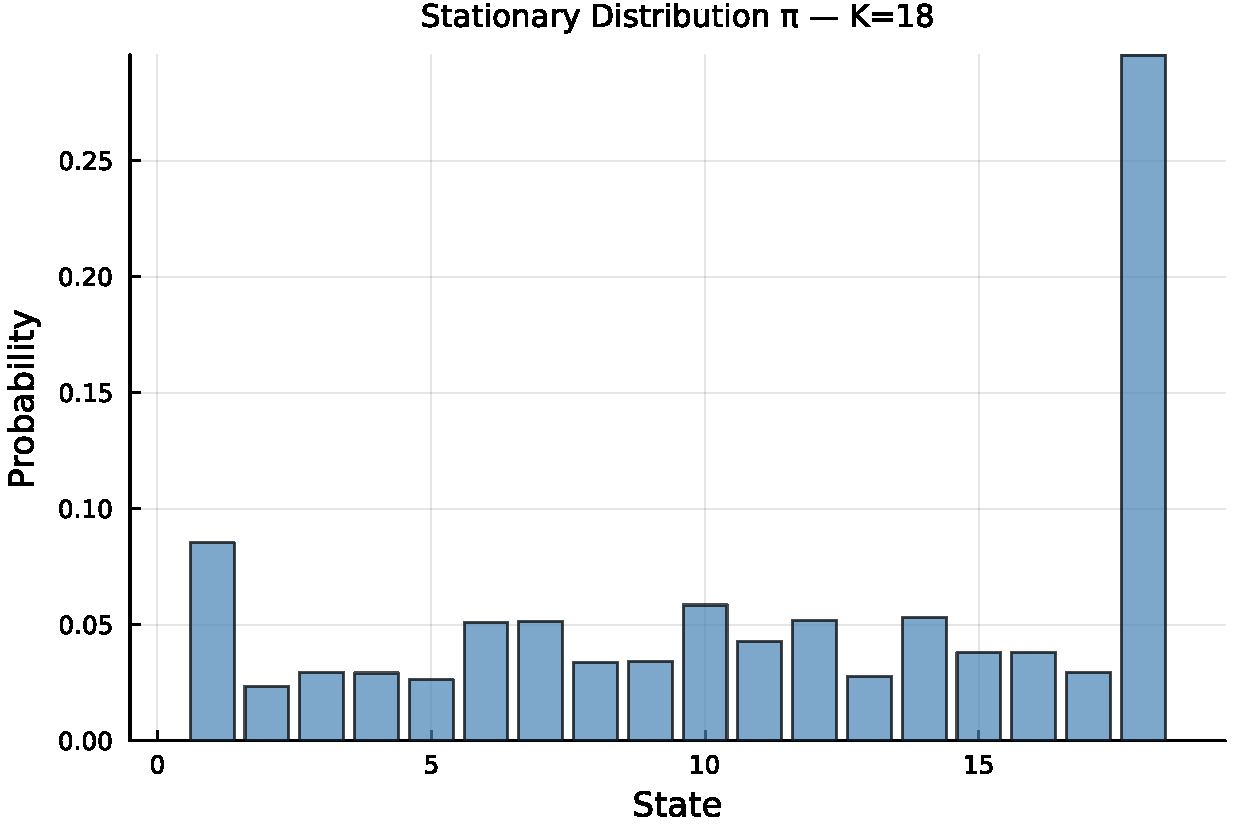
\includegraphics[width=\textwidth]{sections/figs/Fig-Stationary-Distribution-K18.pdf}
    \caption{$K = 18$}
\end{subfigure}
\caption{Stationary distributions $\bar{\boldsymbol{\pi}}$ for $K = 6$ and $K = 18$. Central states receive the highest stationary probability, consistent with the concentration of returns near zero.}
\label{fig:stationary_all}
\end{figure}

\begin{figure}[H]
\centering
\begin{subfigure}[b]{0.48\textwidth}
    
\includegraphics[width=\textwidth]{sections/figs/Fig-Residence-Times-K6.pdf}
    \caption{$K = 6$}
\end{subfigure}
\hfill
\begin{subfigure}[b]{0.48\textwidth}
    
\includegraphics[width=\textwidth]{sections/figs/Fig-Residence-Times-K18.pdf}
    \caption{$K = 18$}
\end{subfigure}
\caption{Natural residence times $\tau_k = 1/(1 - T_{kk})$ per state. Central states have the longest residence times (5--20 days), while tail states are shorter-lived (1--3 days). This asymmetry drives volatility clustering.}
\label{fig:residence_all}
\end{figure}

\subsection{In-Sample Comparison at Non-Selected State Resolutions}
\label{sec:k_sweep_panels}

Figure~\ref{fig:k_sweep_panels_is} shows the in-sample model comparison panels for $K \in \{3, 6, 9, 12, 15, 21\}$, complementing the $K = 18$ comparison in Figure~\ref{fig:is_comparison} of the main text.
Across all resolutions, the CHMM's simulated density closely overlays the observed density, and the ACF of absolute returns tracks the slow decay pattern.
The visible improvement from $K = 3$ to $K = 18$ is concentrated in the tails of the Q-Q panel and the steady-state level of the ACF panel.

\begin{figure}[H]
\centering
\begin{subfigure}[b]{0.32\textwidth}
    
\includegraphics[width=\textwidth]{sections/figs/Fig-3-IS-Comparison-K3.pdf}
    \caption{$K = 3$}
\end{subfigure}
\hfill
\begin{subfigure}[b]{0.32\textwidth}
    
\includegraphics[width=\textwidth]{sections/figs/Fig-3-IS-Comparison-K6.pdf}
    \caption{$K = 6$}
\end{subfigure}
\hfill
\begin{subfigure}[b]{0.32\textwidth}
    
\includegraphics[width=\textwidth]{sections/figs/Fig-3-IS-Comparison-K9.pdf}
    \caption{$K = 9$}
\end{subfigure}

\vspace{0.4cm}

\begin{subfigure}[b]{0.32\textwidth}
    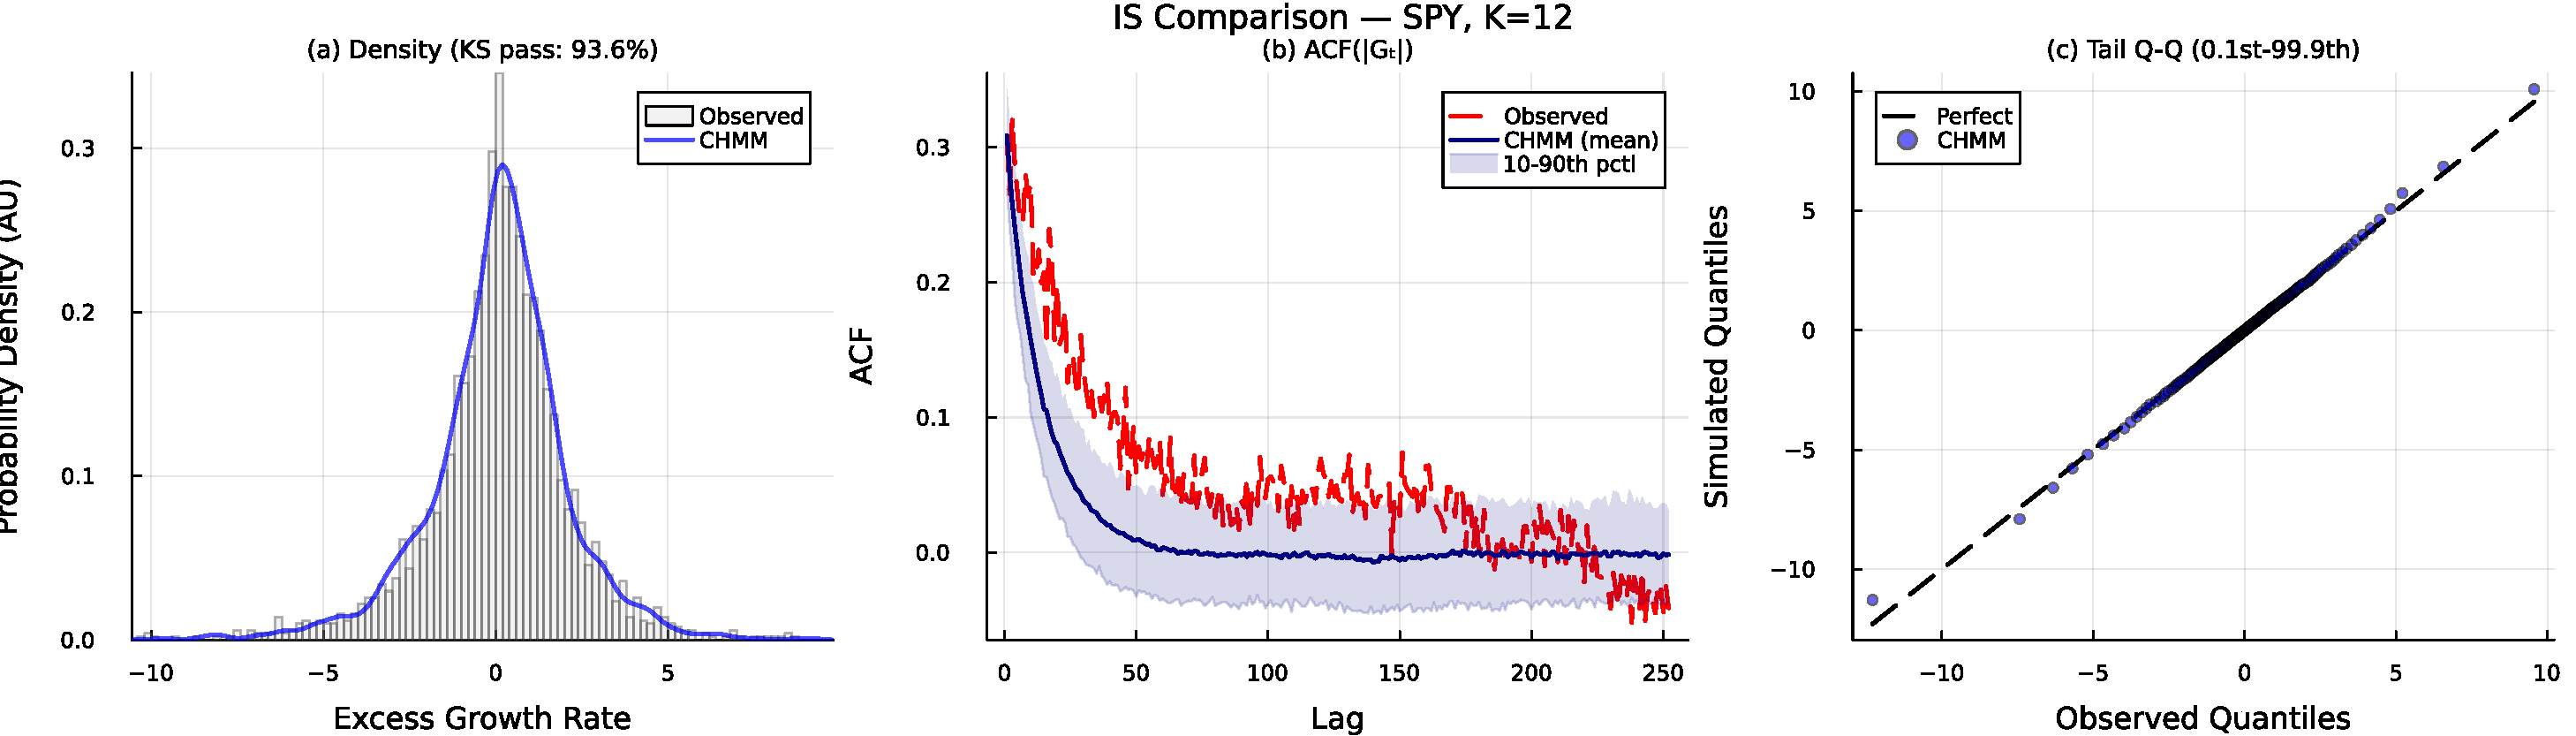
\includegraphics[width=\textwidth]{sections/figs/Fig-3-IS-Comparison-K12.pdf}
    \caption{$K = 12$}
\end{subfigure}
\hfill
\begin{subfigure}[b]{0.32\textwidth}
    
\includegraphics[width=\textwidth]{sections/figs/Fig-3-IS-Comparison-K15.pdf}
    \caption{$K = 15$}
\end{subfigure}
\hfill
\begin{subfigure}[b]{0.32\textwidth}
    
\includegraphics[width=\textwidth]{sections/figs/Fig-3-IS-Comparison-K21.pdf}
    \caption{$K = 21$}
\end{subfigure}
\caption{In-sample CHMM comparison panels at the non-selected state resolutions. Panel $K = 18$ is reproduced in Figure~\ref{fig:is_comparison} of the main text.}
\label{fig:k_sweep_panels_is}
\end{figure}

\subsection{Out-of-Sample Validation at Non-Selected State Resolutions}

Figure~\ref{fig:k_sweep_panels_oos} shows the out-of-sample validation panels for $K \in \{3, 6, 9, 12, 15, 21\}$.
KS pass rates remain above 91\% at all resolutions; the $K = 18$ panel is reproduced in Figure~\ref{fig:oos_validation} of the main text.

\begin{figure}[H]
\centering
\begin{subfigure}[b]{0.32\textwidth}
    
\includegraphics[width=\textwidth]{sections/figs/Fig-4-OoS-Validation-K3.pdf}
    \caption{$K = 3$}
\end{subfigure}
\hfill
\begin{subfigure}[b]{0.32\textwidth}
    
\includegraphics[width=\textwidth]{sections/figs/Fig-4-OoS-Validation-K6.pdf}
    \caption{$K = 6$}
\end{subfigure}
\hfill
\begin{subfigure}[b]{0.32\textwidth}
    
\includegraphics[width=\textwidth]{sections/figs/Fig-4-OoS-Validation-K9.pdf}
    \caption{$K = 9$}
\end{subfigure}

\vspace{0.4cm}

\begin{subfigure}[b]{0.32\textwidth}
    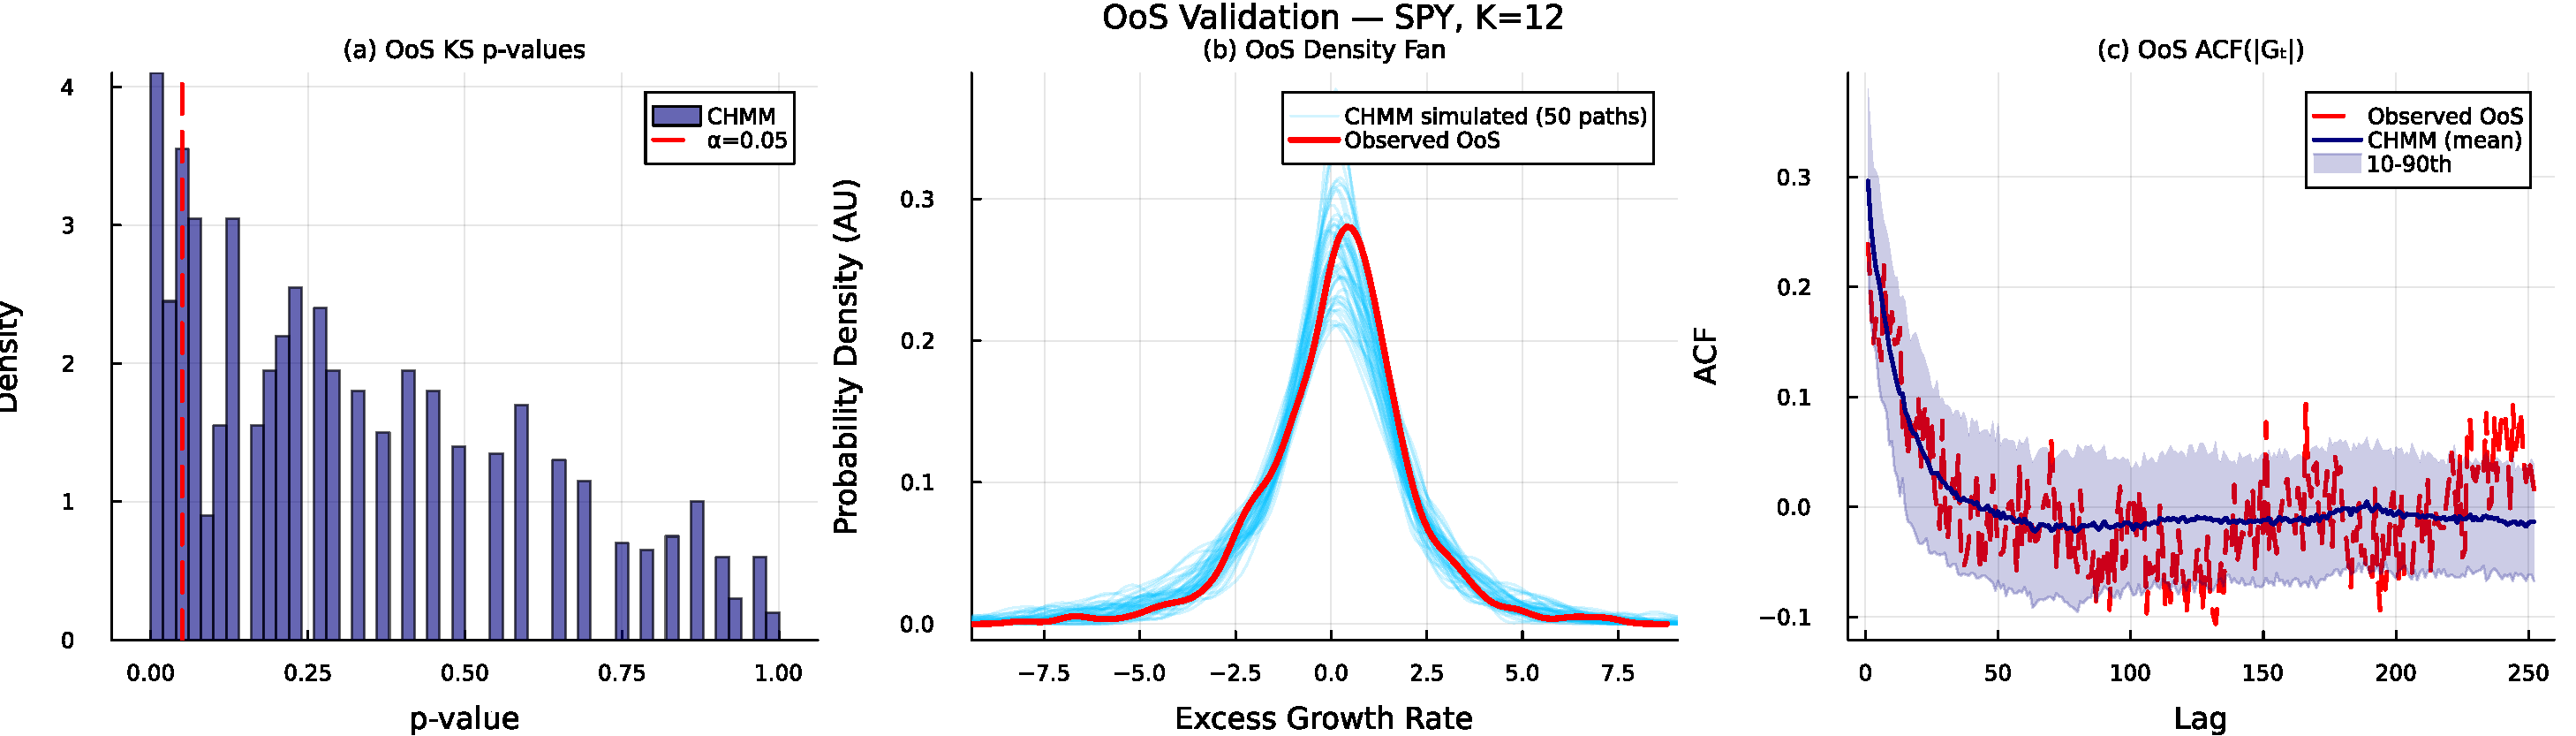
\includegraphics[width=\textwidth]{sections/figs/Fig-4-OoS-Validation-K12.pdf}
    \caption{$K = 12$}
\end{subfigure}
\hfill
\begin{subfigure}[b]{0.32\textwidth}
    
\includegraphics[width=\textwidth]{sections/figs/Fig-4-OoS-Validation-K15.pdf}
    \caption{$K = 15$}
\end{subfigure}
\hfill
\begin{subfigure}[b]{0.32\textwidth}
    
\includegraphics[width=\textwidth]{sections/figs/Fig-4-OoS-Validation-K21.pdf}
    \caption{$K = 21$}
\end{subfigure}
\caption{Out-of-sample CHMM validation panels at the non-selected state resolutions.}
\label{fig:k_sweep_panels_oos}
\end{figure}

\subsection{ACF Comparison Across State Resolutions}

Figure~\ref{fig:acf_all} shows the ACF of $|G_t|$ for the CHMM at $K = 3$, $K = 12$, and $K = 18$, compared to the observed ACF.
At all resolutions, the simulated ACF (shown as the median with 10th--90th percentile envelope across 1{,}000 paths) tracks the observed slow decay pattern.

\begin{figure}[H]
\centering
\begin{subfigure}[b]{0.32\textwidth}
    
\includegraphics[width=\textwidth]{sections/figs/Fig-ACF-Comparison-K3.pdf}
    \caption{$K = 3$}
\end{subfigure}
\hfill
\begin{subfigure}[b]{0.32\textwidth}
    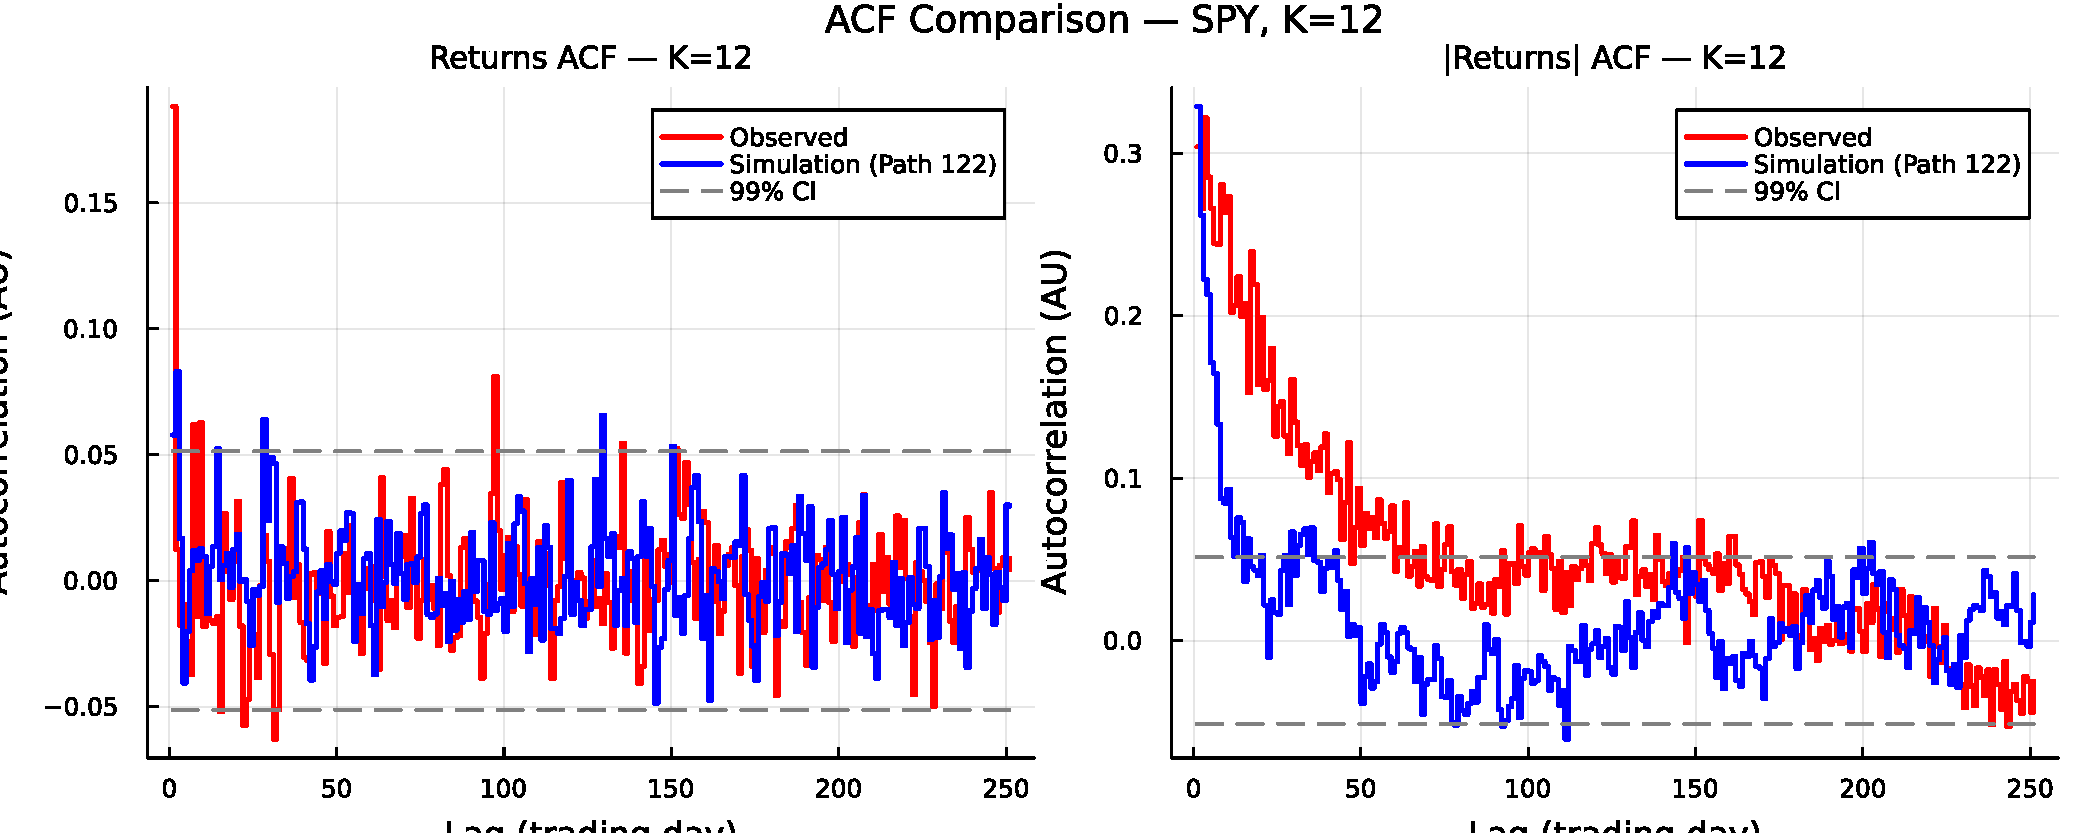
\includegraphics[width=\textwidth]{sections/figs/Fig-ACF-Comparison-K12.pdf}
    \caption{$K = 12$}
\end{subfigure}
\hfill
\begin{subfigure}[b]{0.32\textwidth}
    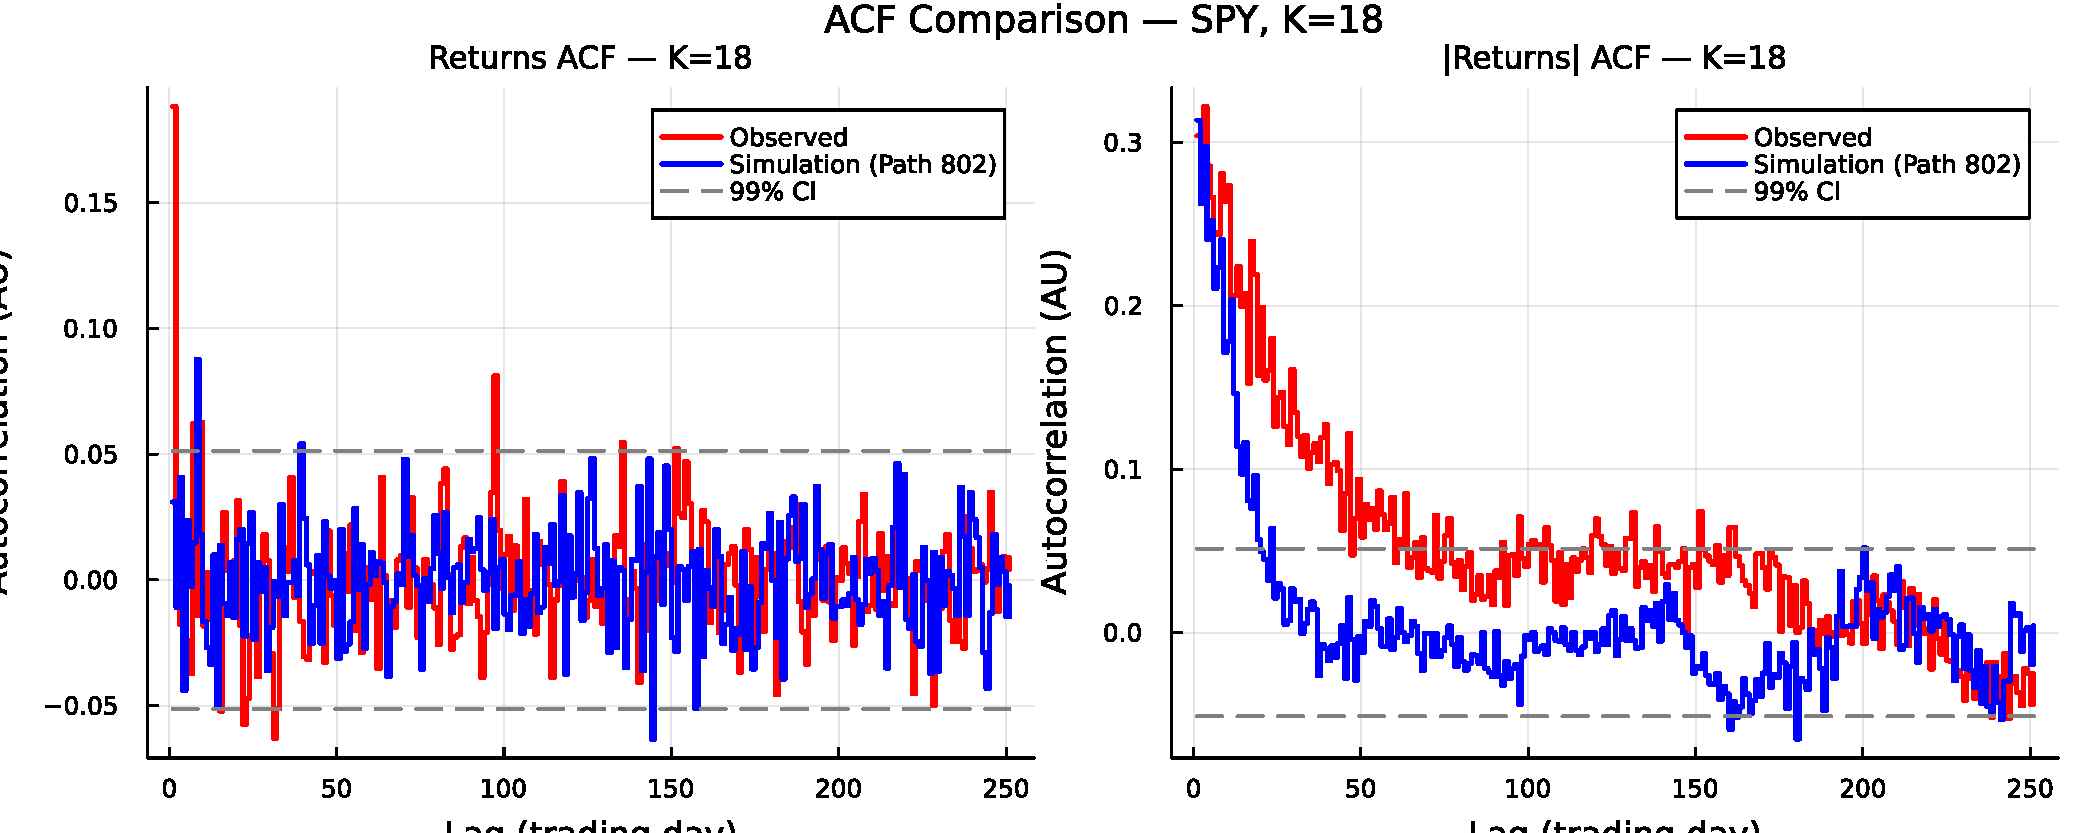
\includegraphics[width=\textwidth]{sections/figs/Fig-ACF-Comparison-K18.pdf}
    \caption{$K = 18$ (selected)}
\end{subfigure}
\caption{ACF of $|G_t|$ for the CHMM at $K = 3$, $K = 12$, and $K = 18$. The simulated 10th--90th percentile envelope (shaded) envelopes the observed ACF (red dashed), confirming that the CHMM reproduces volatility clustering without jump augmentation across the entire sweep.}
\label{fig:acf_all}
\end{figure}

\subsection{Example Simulated Trajectories}

Figure~\ref{fig:trajectories} shows example simulated return trajectories for $K = 6$ and $K = 18$, illustrating the qualitative dynamics produced by the CHMM.
Both trajectories exhibit the characteristic pattern of financial returns: extended periods of low volatility punctuated by clusters of large-magnitude events.

\begin{figure}[H]
\centering
\begin{subfigure}[b]{0.48\textwidth}
    
\includegraphics[width=\textwidth]{sections/figs/Fig-Trajectory-Example-K6.pdf}
    \caption{$K = 6$}
\end{subfigure}
\hfill
\begin{subfigure}[b]{0.48\textwidth}
    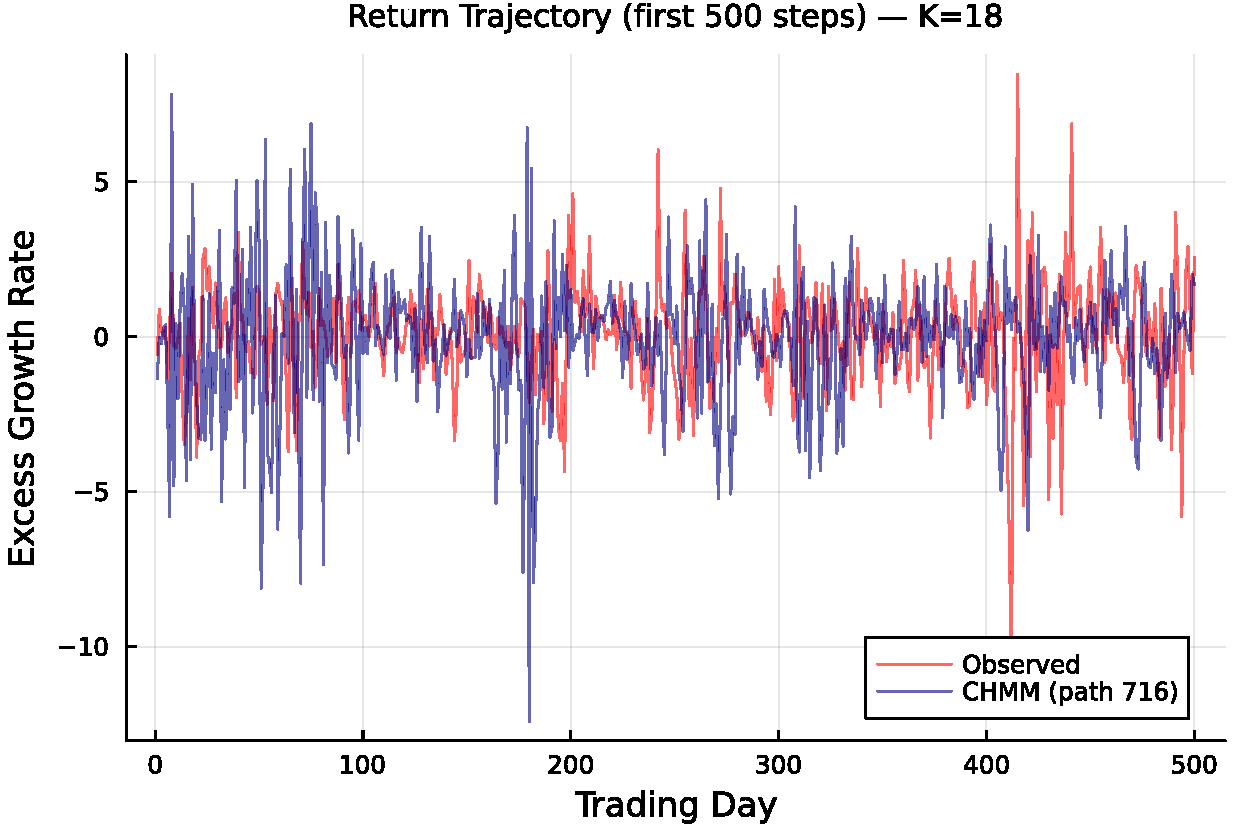
\includegraphics[width=\textwidth]{sections/figs/Fig-Trajectory-Example-K18.pdf}
    \caption{$K = 18$}
\end{subfigure}
\caption{Example simulated return trajectories. The alternation between calm (central states) and volatile (tail states) periods produces the volatility clustering characteristic of empirical financial returns.}
\label{fig:trajectories}
\end{figure}

\subsection{Multi-Emission Figures at $K = 18$}
\label{sec:multi_emission_figs}

This appendix reproduces the standard diagnostic suite (emission PDFs, transition matrix, stationary distribution, residence times, IS comparison, OoS validation, and convergence) for the two heavy-tailed emission families (CHMM-t and CHMM-L) at the selected state resolution $K = 18$.
The Gaussian counterparts are already shown as Figures~\ref{fig:model_internals},~\ref{fig:is_comparison},~\ref{fig:oos_validation},~\ref{fig:convergence_all},~\ref{fig:transition_all},~\ref{fig:stationary_all}, and~\ref{fig:residence_all} in the main text and above in this appendix.
The figures confirm that the shared forward--backward scaffold produces internally-similar regime structure across the three families: the near-diagonal transition band, the $K$-component dense emission cover, the longer central-state residence times, and the monotone log-likelihood convergence are features of the CHMM framework and not of the Gaussian component specifically.

\paragraph{Emission PDFs.}
Figure~\ref{fig:emissions_families} compares the learned $K = 18$ emissions for the three families.
The CHMM-t panel's per-state $\nu_k$ allocation is visible in the narrower modes of certain tail states; the CHMM-L panel's Laplace components have sharper peaks and slower exponential tail decay than the Gaussians.

\begin{figure}[H]
\centering
\begin{subfigure}[b]{0.32\textwidth}
    
\includegraphics[width=\textwidth]{sections/figs/Fig-Emission-PDFs-K18-N.pdf}
    \caption{CHMM-N (Gaussian)}
\end{subfigure}
\hfill
\begin{subfigure}[b]{0.32\textwidth}
    
\includegraphics[width=\textwidth]{sections/figs/Fig-Emission-PDFs-K18-t.pdf}
    \caption{CHMM-t (Student-t)}
\end{subfigure}
\hfill
\begin{subfigure}[b]{0.32\textwidth}
    
\includegraphics[width=\textwidth]{sections/figs/Fig-Emission-PDFs-K18-L.pdf}
    \caption{CHMM-L (Laplace)}
\end{subfigure}
\caption{Learned emission distributions at $K = 18$ across the three emission families, overlaid on the observed SPY return histogram. Heavier-tailed emission families (t, L) give individual components more tail mass, which is what closes the kurtosis gap of the Gaussian CHMM.}
\label{fig:emissions_families}
\end{figure}

\paragraph{Transition matrices.}
Figure~\ref{fig:transition_families} shows the $K = 18$ transition matrices learned by each family.
The near-diagonal band and the magnitude of self-transition probabilities are essentially unchanged across families, consistent with the ACF-MAE being stable across the family axis (Table~\ref{tab:sensitivity_multi}).

\begin{figure}[H]
\centering
\begin{subfigure}[b]{0.32\textwidth}
    
\includegraphics[width=\textwidth]{sections/figs/Fig-Transition-Matrix-K18-N.pdf}
    \caption{CHMM-N}
\end{subfigure}
\hfill
\begin{subfigure}[b]{0.32\textwidth}
    
\includegraphics[width=\textwidth]{sections/figs/Fig-Transition-Matrix-K18-t.pdf}
    \caption{CHMM-t}
\end{subfigure}
\hfill
\begin{subfigure}[b]{0.32\textwidth}
    
\includegraphics[width=\textwidth]{sections/figs/Fig-Transition-Matrix-K18-L.pdf}
    \caption{CHMM-L}
\end{subfigure}
\caption{Learned transition matrices at $K = 18$ in log$_{10}$ color scale. The diagonal-band structure is preserved across all three emission families.}
\label{fig:transition_families}
\end{figure}

\paragraph{Stationary distributions and residence times.}
Figure~\ref{fig:stationary_families} and Figure~\ref{fig:residence_families} compare the stationary distribution and natural residence times $\tau_k = 1/(1 - T_{kk})$ across families at $K = 18$.
The mass concentration at central states and the monotone decrease of $\tau_k$ toward the tails are features of the regime structure, not the emission family.

\begin{figure}[H]
\centering
\begin{subfigure}[b]{0.32\textwidth}
    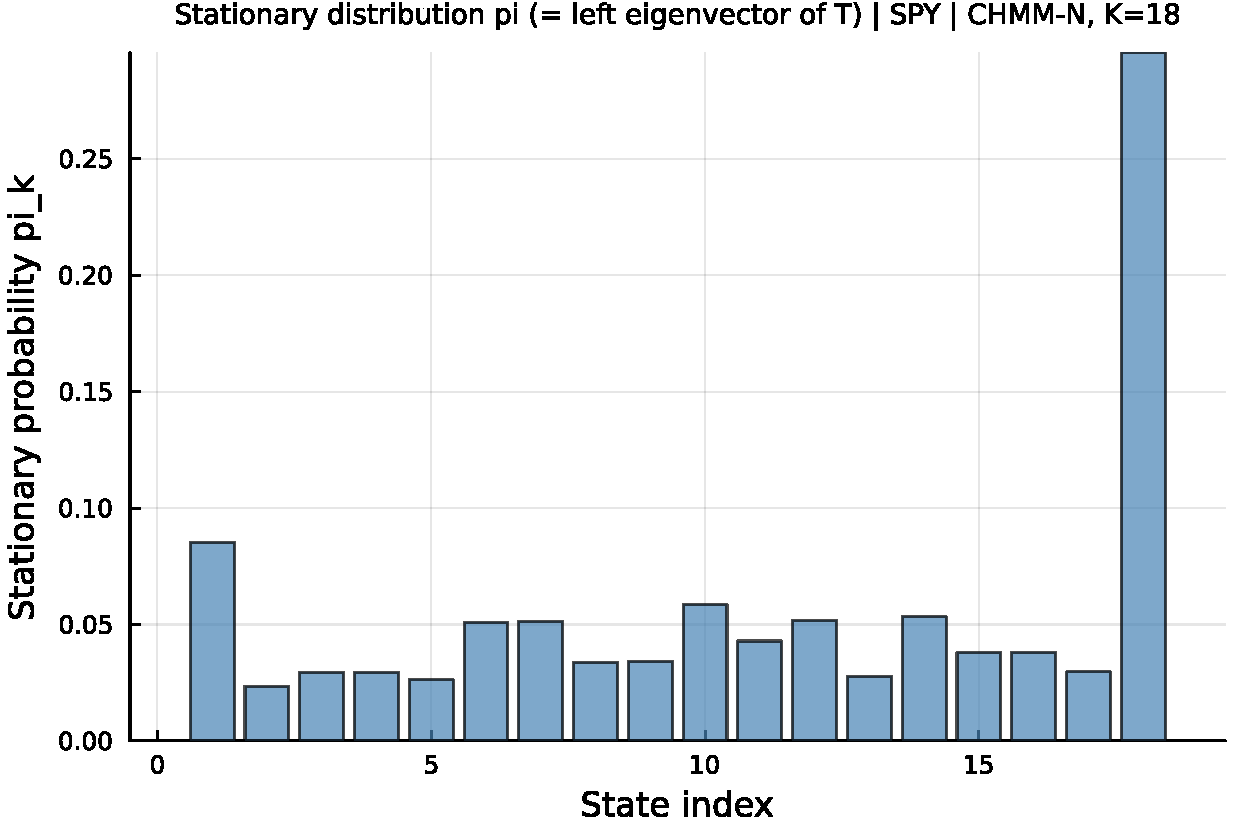
\includegraphics[width=\textwidth]{sections/figs/Fig-Stationary-Distribution-K18-N.pdf}
    \caption{CHMM-N}
\end{subfigure}
\hfill
\begin{subfigure}[b]{0.32\textwidth}
    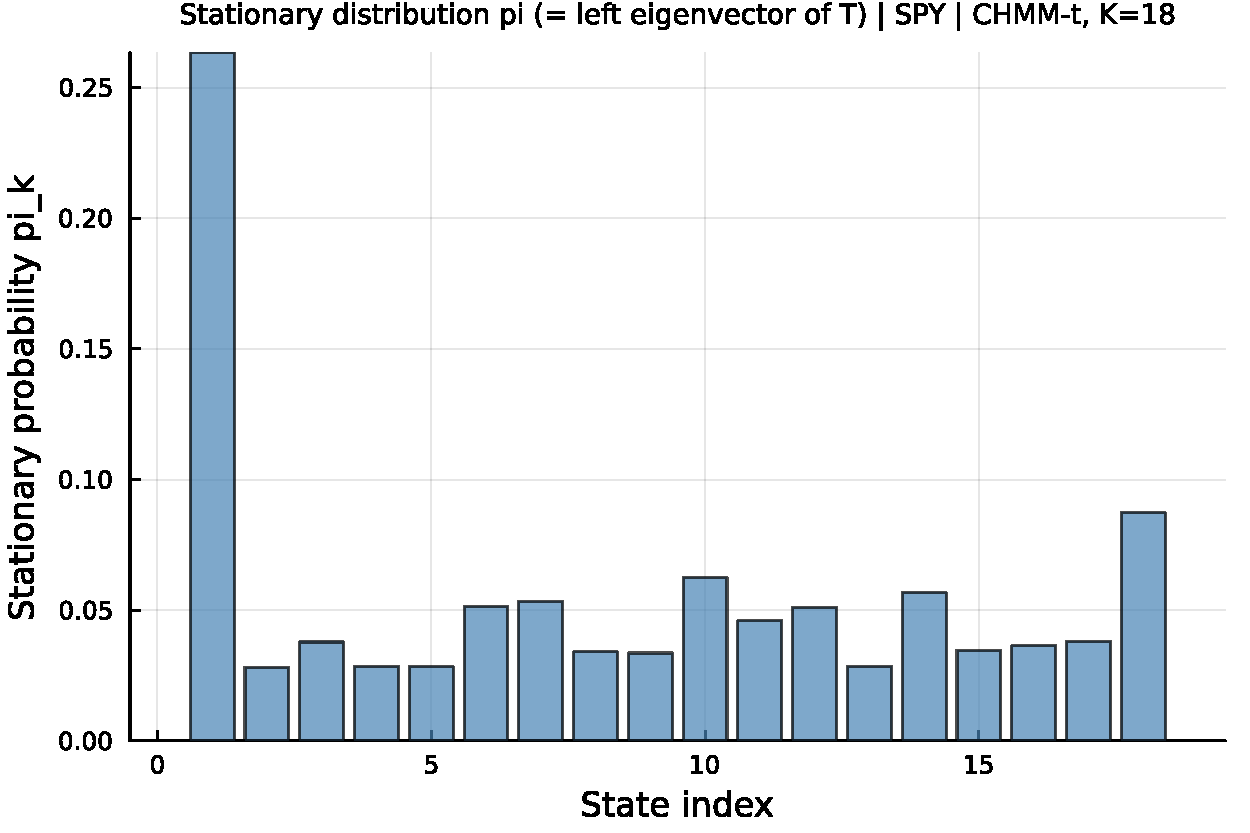
\includegraphics[width=\textwidth]{sections/figs/Fig-Stationary-Distribution-K18-t.pdf}
    \caption{CHMM-t}
\end{subfigure}
\hfill
\begin{subfigure}[b]{0.32\textwidth}
    
\includegraphics[width=\textwidth]{sections/figs/Fig-Stationary-Distribution-K18-L.pdf}
    \caption{CHMM-L}
\end{subfigure}
\caption{Stationary distributions $\bar{\boldsymbol{\pi}}$ at $K = 18$ across the three emission families.}
\label{fig:stationary_families}
\end{figure}

\begin{figure}[H]
\centering
\begin{subfigure}[b]{0.32\textwidth}
    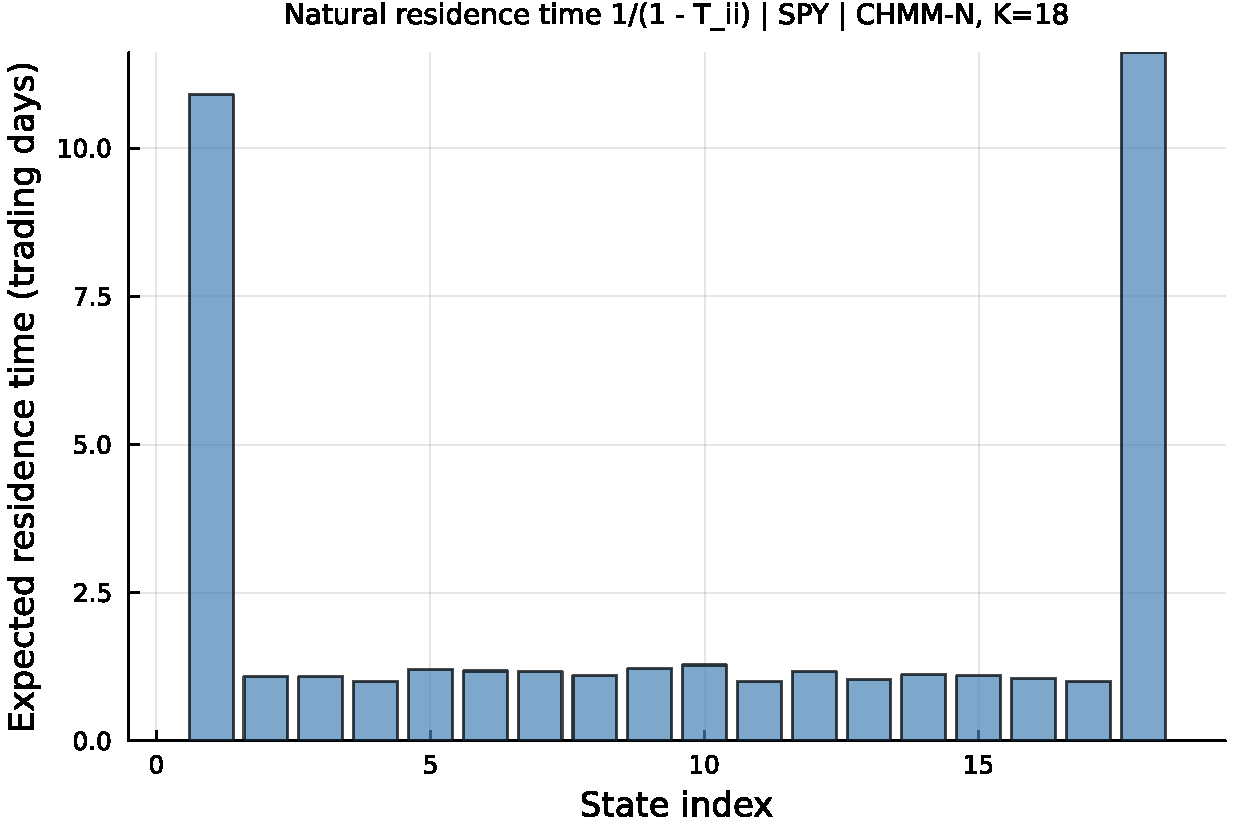
\includegraphics[width=\textwidth]{sections/figs/Fig-Residence-Times-K18-N.pdf}
    \caption{CHMM-N}
\end{subfigure}
\hfill
\begin{subfigure}[b]{0.32\textwidth}
    
\includegraphics[width=\textwidth]{sections/figs/Fig-Residence-Times-K18-t.pdf}
    \caption{CHMM-t}
\end{subfigure}
\hfill
\begin{subfigure}[b]{0.32\textwidth}
    
\includegraphics[width=\textwidth]{sections/figs/Fig-Residence-Times-K18-L.pdf}
    \caption{CHMM-L}
\end{subfigure}
\caption{Natural residence times $\tau_k = 1/(1 - T_{kk})$ at $K = 18$ across the three emission families.}
\label{fig:residence_families}
\end{figure}

\paragraph{In-sample comparison.}
Figure~\ref{fig:is_families} reproduces the three-panel in-sample comparison (density, ACF of $|G_t|$, tail Q-Q) at $K = 18$ for the two heavy-tailed families; the CHMM-N panel is Figure~\ref{fig:is_comparison} in the main text.

\begin{figure}[H]
\centering
\begin{subfigure}[b]{0.48\textwidth}
    
\includegraphics[width=\textwidth]{sections/figs/Fig-3-IS-Comparison-K18-t.pdf}
    \caption{CHMM-t}
\end{subfigure}
\hfill
\begin{subfigure}[b]{0.48\textwidth}
    
\includegraphics[width=\textwidth]{sections/figs/Fig-3-IS-Comparison-K18-L.pdf}
    \caption{CHMM-L}
\end{subfigure}
\caption{In-sample model comparison at $K = 18$ for the two heavy-tailed emission families. Each panel shows (a) marginal density with KS pass rate, (b) ACF of $|G_t|$, and (c) tail Q-Q plot. The CHMM-N counterpart is Figure~\ref{fig:is_comparison}.}
\label{fig:is_families}
\end{figure}

\paragraph{Out-of-sample validation.}
Figure~\ref{fig:oos_families} shows the OoS validation panels for CHMM-t and CHMM-L at $K = 18$.
The CHMM-t panel demonstrates the OoS kurtosis alignment noted in the main text (simulated 6.40 vs.\ observed 6.24), and the CHMM-L panel shows the tighter density fan produced by the heavier Laplace tails relative to the Gaussian.

\begin{figure}[H]
\centering
\begin{subfigure}[b]{0.48\textwidth}
    
\includegraphics[width=\textwidth]{sections/figs/Fig-4-OoS-Validation-K18-t.pdf}
    \caption{CHMM-t}
\end{subfigure}
\hfill
\begin{subfigure}[b]{0.48\textwidth}
    
\includegraphics[width=\textwidth]{sections/figs/Fig-4-OoS-Validation-K18-L.pdf}
    \caption{CHMM-L}
\end{subfigure}
\caption{Out-of-sample validation at $K = 18$ for the two heavy-tailed emission families. Each panel shows (a) KS $p$-values, (b) OoS density fan, and (c) OoS ACF of $|G_t|$. The CHMM-N counterpart is Figure~\ref{fig:oos_validation}.}
\label{fig:oos_families}
\end{figure}

\paragraph{Convergence.}
Figure~\ref{fig:convergence_families} shows the Baum-Welch / ECM / weighted-EM log-likelihood histories at $K = 18$ for all three families.
The CHMM-t and CHMM-L curves inherit the monotone increase of the classical EM guarantee; the CHMM-t curve has a slightly longer pre-plateau phase because each ECM sub-iteration refines $\nu_k$ with a golden-section search.

\begin{figure}[H]
\centering
\begin{subfigure}[b]{0.32\textwidth}
    
\includegraphics[width=\textwidth]{sections/figs/Fig-Convergence-K18-N.pdf}
    \caption{CHMM-N}
\end{subfigure}
\hfill
\begin{subfigure}[b]{0.32\textwidth}
    
\includegraphics[width=\textwidth]{sections/figs/Fig-Convergence-K18-t.pdf}
    \caption{CHMM-t}
\end{subfigure}
\hfill
\begin{subfigure}[b]{0.32\textwidth}
    
\includegraphics[width=\textwidth]{sections/figs/Fig-Convergence-K18-L.pdf}
    \caption{CHMM-L}
\end{subfigure}
\caption{Log-likelihood histories at $K = 18$ across the three emission families. All three curves are monotonically non-decreasing and plateau well before the $\texttt{max\_iter} = 60$ budget.}
\label{fig:convergence_families}
\end{figure}

\subsection{Cross-Asset Dependence Models: Derivations and Diagnostics (Pipeline B)}
\label{sec:cross_asset_supp}

This appendix provides the technical background for the SIM and copula constructions used in Section~\ref{sec:cross_asset} of the main text. These constructions constitute \emph{Pipeline B}: per-asset marginals come from the independent CHMMs of Pipeline A (Section~\ref{sec:cross_asset_univariate}) and joint dependence is overlaid on top. Pipeline A stays purely univariate; Pipeline B is the sole multi-asset pipeline in the paper.

\paragraph{Sklar's theorem and the rank-reordering simulator.}
Sklar's theorem \cite{sklar1959fonctions, nelsen2006introduction} states that any $d$-dimensional joint CDF $H(g_1, \dots, g_d)$ with continuous marginals $F_1, \dots, F_d$ can be written as $H = C(F_1, \dots, F_d)$ for a unique copula $C$.
The rank-reordering simulator exploits this uniqueness.
If $\tilde{\mathbf{G}}$ is a matrix whose $j$-th column is an i.i.d.\ sample from $F_j$, and $\mathbf{U}$ is an independent sample from $C$, then reordering each column of $\tilde{\mathbf{G}}$ so that its ranks match $\mathbf{U}$'s produces a sample from $H$, up to discrete approximation error in the empirical ranks.
Crucially, reordering never creates new values: each column of the output is a permutation of the corresponding column of $\tilde{\mathbf{G}}$, so marginal distributions are preserved exactly \cite{iman1982distribution}.

\paragraph{Kendall's $\tau$ inversion.}
Given in-sample returns $\mathbf{R} \in \mathbb{R}^{T \times d}$, we estimate the pairwise Kendall's $\tau_{ij}$ from concordant/discordant pair counts and invert to the correlation scale via the analytic relationship $\rho_{ij} = \sin(\pi \tau_{ij} / 2)$, which holds exactly for the Gaussian copula family and is commonly used as a robust correlation estimator for the Student-t copula \cite{embrechts2002correlation, mcneil2015quantitative}.
The resulting matrix $\hat{\Sigma}$ is symmetric but not guaranteed positive semi-definite; we project to the nearest PSD matrix by clipping negative eigenvalues to $10^{-8}$ and rescaling the diagonal to unity.

\paragraph{Profile MLE for $\nu$.}
The Student-t copula log-density at a single pseudo-uniform observation $\mathbf{u} \in [0,1]^d$, with $x_j = t_\nu^{-1}(u_j)$ and $\mathbf{x} = (x_1, \dots, x_d)^\top$, is
\begin{align}
    \log c_t(\mathbf{u}; \Sigma, \nu)
    \;=\;&
    \log \Gamma\!\left(\tfrac{\nu+d}{2}\right)
    + (d-1)\,\log \Gamma\!\left(\tfrac{\nu}{2}\right)
    - d\,\log \Gamma\!\left(\tfrac{\nu+1}{2}\right)
    - \tfrac{1}{2} \log |\Sigma|
    \notag \\
    &\;
    - \tfrac{\nu+d}{2}\,\log\!\left(1 + \tfrac{\mathbf{x}^{\!\top} \Sigma^{-1} \mathbf{x}}{\nu}\right)
    + \sum_{j=1}^{d} \tfrac{\nu+1}{2}\,\log\!\left(1 + \tfrac{x_j^2}{\nu}\right).
    \label{eq:tcop_ll}
\end{align}
Summing over $t = 1, \dots, T$ pseudo-observations yields the profile log-likelihood as a function of $\nu$ with $\Sigma$ held fixed at the Kendall's-$\tau$ estimate.
We evaluate equation~\eqref{eq:tcop_ll} on the discrete grid $\nu \in \{2, 3, 4, 5, 6, 8, 10, 15, 20, 30\}$ and select $\hat{\nu}$ as the grid point with the largest total log-likelihood.
In Section~\ref{sec:cross_asset} the selected value was $\hat{\nu} = 6$ on the six-asset universe.

\paragraph{Sampling the copula.}
To sample $T$ rows from the $d$-dimensional Gaussian copula with correlation $\Sigma$, we (i) compute the Cholesky factor $\Sigma = L L^\top$, (ii) draw $Z \sim \mathcal{N}(0, I_d)$ i.i.d.\ and form $Y = L Z$, and (iii) return $U = \Phi(Y)$ componentwise.
For the Student-t copula with degrees of freedom $\nu$, we draw $W \sim \chi^2_\nu / \nu$ independent of $Y$ and form the multivariate-$t$ variate $X = Y / \sqrt{W}$, then return $U = t_\nu(X)$ componentwise.

\paragraph{SIM regression summary.}
Table~\ref{tab:sim_regression} reports the fitted SIM regression coefficients and goodness-of-fit statistics for the non-market assets in Section~\ref{sec:cross_asset}.
QQQ's high $R^2 = 0.840$ reflects that the Nasdaq-100 ETF is essentially a linear combination of large-cap technology names that also drive the S\&P~500 index, while JNJ's lower $R^2 = 0.260$ reflects the limited systematic exposure of low-beta healthcare stocks.
These factor loadings and residual magnitudes are what the SIM simulation in equation~\eqref{eq:sim_sim} re-injects at simulation time, and they explain the uneven per-asset KS pass rates reported in Table~\ref{tab:cross_asset_sim_copula}.

\begin{table}[H]
\centering
\caption{SIM regression $\hat{G}_{j,t} = \hat{\alpha}_j + \hat{\beta}_j G_{\text{SPY},t} + \hat{\eta}_{j,t}$ for the five non-market assets, fitted on the $2014$-$01$-$03$ through $2024$-$01$-$03$ in-sample window ($T = 2{,}516$). Coefficients $\hat{\alpha}, \hat{\beta}$ and $R^2$ are reported for the factor equation used in equation~\eqref{eq:sim_sim}.}
\label{tab:sim_regression}
\small
\begin{tabular}{l ccc}
\toprule
Ticker & $\hat{\alpha}$ & $\hat{\beta}$ & $R^2$ \\
\midrule
NVDA & $0.321$   & $1.694$ & $0.371$ \\
JNJ  & $0.002$   & $0.576$ & $0.260$ \\
JPM  & $-0.008$  & $1.223$ & $0.507$ \\
AAPL & $0.111$   & $1.205$ & $0.492$ \\
QQQ  & $0.047$   & $1.122$ & $0.840$ \\
\bottomrule
\end{tabular}
\end{table}

\subsection{Algorithm Descriptions}
\label{sec:algorithms}

This section provides detailed pseudocode for the main algorithms used in this study.
Algorithm~\ref{alg:chmm_em} is the unified EM procedure shared across all three emission families.
It makes explicit the \emph{shared scaffold} (quantile-based initialization, log-space forward-backward, transition update) and the three \emph{family-specific branches} (Gaussian M-step for CHMM-N, ECM with one-dimensional golden-section $\nu$-search for CHMM-t, closed-form weighted-median + weighted-MAD for CHMM-L); the branch points are lines~\ref{line:init}, \ref{line:emit}, and \ref{line:mstep}.
Visualizing the three variants as a single algorithm with three M-step branches makes the architectural contribution of the paper --- one EM engine, three interchangeable emission families --- immediate from the pseudocode.
Algorithm~\ref{alg:viterbi} presents the Viterbi algorithm for decoding the most likely hidden state sequence.
Algorithm~\ref{alg:chmm_simulate} describes the CHMM simulation procedure for generating synthetic return paths.
Algorithm~\ref{alg:copula_sim} describes the cross-asset rank-reordering simulator for copula-based multi-asset synthesis.
Algorithm~\ref{alg:sim_build} details the SIM regression-and-resampling pipeline.

% ========================================================================================= %
% Algorithm 1: Baum-Welch (EM) for Continuous Gaussian HMM
% ========================================================================================= %
% Unified EM algorithm with family-specific M-step switch
% ========================================================================================= %
\begin{algorithm}[tp]
\caption{Unified EM algorithm for the CHMM family. Lines~\ref{line:init}, \ref{line:emit}, and \ref{line:mstep} branch on the emission family $F \in \{\mathcal{N}, t, L\}$; every other line is identical across families. CHMM-N and CHMM-L instantiate classical EM; CHMM-t instantiates an ECM sequence whose second CM step updates $\nu_k$ by a one-dimensional golden-section search on the per-state $Q$-function.}
\label{alg:chmm_em}
\small
\begin{algorithmic}[1]
\REQUIRE Observations $O_{1:T}$, number of states $K$, tolerance $\text{tol}$, $\texttt{max\_iter}$, emission family $F \in \{\mathcal{N}, t, L\}$, if $F = t$ bracket $(\nu_{\min}, \nu_{\max})$ and initial $\nu^{(0)}$.
\ENSURE Transition matrix $\mathbf{T}$, per-state emission parameters $\boldsymbol\theta_{1:K}$, initial distribution $\boldsymbol{\pi}$.

\STATE \textbf{Quantile-Based Initialization.}
\STATE Sort $O^{(\text{sort})} \leftarrow \text{sort}(O_{1:T})$ and partition into $K$ equal chunks $\{C_1,\ldots,C_K\}$.
\FOR{$k = 1$ to $K$} \label{line:init}
    \STATE \textbf{switch} $F$
    \STATE \quad $F = \mathcal{N}$: $\mu_k \leftarrow \text{mean}(C_k)$, \quad $\sigma_k \leftarrow \max(\text{std}(C_k), 10^{-6})$.
    \STATE \quad $F = t$: $\mu_k \leftarrow \text{mean}(C_k)$, \quad $\sigma_k \leftarrow \max(\text{std}(C_k), 10^{-6})$, \quad $\nu_k \leftarrow \nu^{(0)}$.
    \STATE \quad $F = L$: $\mu_k \leftarrow \text{median}(C_k)$, \quad $b_k \leftarrow \max(\text{mean}(|C_k - \mu_k|), 10^{-6})$.
\ENDFOR
\STATE $T_{ij} \leftarrow 1/K$; \quad $\pi_k \leftarrow 1/K$; \quad $\mathcal{L}_{\text{prev}} \leftarrow -\infty$.

\STATE \textbf{EM Loop.}
\FOR{$n = 1$ to $\texttt{max\_iter}$}

    \STATE \textbf{E-Step --- per-family emission log-likelihood.} \label{line:emit}
    \STATE \textbf{switch} $F$
    \STATE \quad $F = \mathcal{N}$: $\log B_{t,k} \leftarrow \log \mathcal{N}(O_t \mid \mu_k, \sigma_k^2)$.
    \STATE \quad $F = t$: $\log B_{t,k} \leftarrow \log t_{\nu_k}(O_t; \mu_k, \sigma_k)$.
    \STATE \quad $F = L$: $\log B_{t,k} \leftarrow -\log(2 b_k) - |O_t - \mu_k|/b_k$.

    \STATE \textbf{E-Step --- shared log-space forward-backward.}
    \STATE $\log \alpha_1(k) \leftarrow \log \pi_k + \log B_{1,k}$.
    \FOR{$t = 2$ to $T$, $j = 1$ to $K$}
        \STATE $\log \alpha_t(j) \leftarrow \underset{i}{\text{logsumexp}}\!\left(\log \alpha_{t-1}(i) + \log T_{ij}\right) + \log B_{t,j}$.
    \ENDFOR
    \STATE $\log \beta_T(k) \leftarrow 0$.
    \FOR{$t = T-1$ down to $1$, $i = 1$ to $K$}
        \STATE $\log \beta_t(i) \leftarrow \underset{j}{\text{logsumexp}}\!\left(\log T_{ij} + \log B_{t+1,j} + \log \beta_{t+1}(j)\right)$.
    \ENDFOR
    \STATE Compute $\gamma_t(k)$ and $\xi_t(i,j)$ from equation~\eqref{eq:gamma_xi}.

    \STATE \textbf{Shared transition update.} $T_{ij} \leftarrow \sum_t \xi_t(i,j) \;/\; \sum_t \gamma_t(i)$; $\pi_k \leftarrow \gamma_1(k)$.

    \STATE \textbf{M-Step --- per-family emission update.} \label{line:mstep}
    \STATE \textbf{switch} $F$
    \STATE \quad $F = \mathcal{N}$ \COMMENT{classical Baum-Welch \citep{baum1970maximization}.}
    \STATE \qquad $\mu_k \leftarrow \sum_t \gamma_t(k)\, O_t / \sum_t \gamma_t(k)$.
    \STATE \qquad $\sigma_k \leftarrow \max\!\left(\sqrt{\sum_t \gamma_t(k) (O_t - \mu_k)^2 / \sum_t \gamma_t(k)},\; 10^{-6}\right)$.
    \STATE \quad $F = t$ \COMMENT{ECM of \citet{peel2000robust, liu1995ml}; closed-form $(\mu_k, \sigma_k)$ given $\nu_k$, then 1D search on $\nu_k$.}
    \STATE \qquad $u_{t,k} \leftarrow (\nu_k + 1) / (\nu_k + ((O_t - \mu_k)/\sigma_k)^2)$ for all $t, k$.
    \STATE \qquad $\mu_k \leftarrow \sum_t \gamma_t(k)\, u_{t,k}\, O_t / \sum_t \gamma_t(k)\, u_{t,k}$.
    \STATE \qquad $\sigma_k \leftarrow \max\!\left(\sqrt{\sum_t \gamma_t(k)\, u_{t,k}\,(O_t - \mu_k)^2 / \sum_t \gamma_t(k)},\; 10^{-6}\right)$.
    \STATE \qquad $\nu_k \leftarrow \arg\max_{\nu \in [\nu_{\min}, \nu_{\max}]} \sum_t \gamma_t(k)\, \log t_\nu(O_t; \mu_k, \sigma_k)$ \COMMENT{40-iter golden-section search.}
    \STATE \quad $F = L$ \COMMENT{closed-form weighted Laplace MLE.}
    \STATE \qquad $\mu_k \leftarrow \text{WeightedMedian}(O_{1:T},\, \gamma_{1:T}(k))$ \COMMENT{cumulative-weight bracketing with interpolation at the $W_k/2$ crossing.}
    \STATE \qquad $b_k \leftarrow \max\!\left(\sum_t \gamma_t(k)\, |O_t - \mu_k| / \sum_t \gamma_t(k),\; 10^{-6}\right)$.

    \STATE \textbf{Convergence check.} $\mathcal{L}^{(n)} \leftarrow \underset{k}{\text{logsumexp}}(\log \alpha_T(k))$.
    \IF{$|\mathcal{L}^{(n)} - \mathcal{L}_{\text{prev}}| < \text{tol}$} \STATE \textbf{break} \ENDIF
    \STATE $\mathcal{L}_{\text{prev}} \leftarrow \mathcal{L}^{(n)}$.
\ENDFOR

\RETURN $\mathbf{T}, \boldsymbol\theta_{1:K}, \boldsymbol{\pi}$ \COMMENT{$\boldsymbol\theta_k = (\mu_k, \sigma_k)$ for $F = \mathcal{N}$; $(\mu_k, \sigma_k, \nu_k)$ for $F = t$; $(\mu_k, b_k)$ for $F = L$.}
\end{algorithmic}
\end{algorithm}

% Backward-compatibility labels: any older cross-reference to the separate algorithms now points at the unified block.
\newcommand{\algbaumwelch}{\ref{alg:chmm_em}}
\newcommand{\algecmstudentt}{\ref{alg:chmm_em}}
\newcommand{\algemlaplace}{\ref{alg:chmm_em}}

% ========================================================================================= %
% Algorithm 2: Viterbi Decoding
% ========================================================================================= %
\begin{algorithm}[tp]
\caption{Viterbi decoding for the most likely hidden state sequence}
\label{alg:viterbi}
\small
\begin{algorithmic}[1]
\REQUIRE Observations $O_{1:T}$, Trained CHMM $\mathcal{M} = (\mathbf{T}, \{\mu_k, \sigma_k\}, \boldsymbol{\pi})$
\ENSURE Most probable state sequence $S_{1:T}^*$

\FOR{$k = 1$ to $K$}
    \STATE $\log \delta_1(k) \leftarrow \log(1/K) + \log \mathcal{N}(O_1 \mid \mu_k, \sigma_k^2)$.
\ENDFOR

\FOR{$t = 2$ to $T$}
    \FOR{$j = 1$ to $K$}
        \STATE $\text{vals}(i) \leftarrow \log \delta_{t-1}(i) + \log T_{ij}$ for all $i$.
        \STATE $\log \delta_t(j) \leftarrow \max_i \text{vals}(i) + \log \mathcal{N}(O_t \mid \mu_j, \sigma_j^2)$.
        \STATE $\psi_t(j) \leftarrow \arg\max_i \text{vals}(i)$.
    \ENDFOR
\ENDFOR

\STATE $S_T^* \leftarrow \arg\max_k \log \delta_T(k)$.
\FOR{$t = T-1$ down to $1$}
    \STATE $S_t^* \leftarrow \psi_{t+1}(S_{t+1}^*)$.
\ENDFOR

\RETURN $S_{1:T}^*$
\end{algorithmic}
\end{algorithm}

% ========================================================================================= %
% Algorithm 3: CHMM Simulation
% ========================================================================================= %
\begin{algorithm}[tp]
\caption{CHMM simulation of synthetic excess growth rate paths}
\label{alg:chmm_simulate}
\small
\begin{algorithmic}[1]
\REQUIRE Trained CHMM $\mathcal{M} = (\mathbf{T}, \{\mu_k, \sigma_k\}, \boldsymbol{\pi})$, Number of steps $M$, Number of paths $P$
\ENSURE Simulated return paths $\{\hat{G}^{(p)}_{1:M}\}_{p=1}^{P}$

\FOR{$p = 1$ to $P$}
    \STATE Sample initial state $S_1 \sim \text{Categorical}(\boldsymbol{\pi})$.
    \FOR{$t = 1$ to $M$}
        \STATE Emit observation $\hat{G}_t^{(p)} \sim \mathcal{N}(\mu_{S_t}, \sigma_{S_t}^2)$.
        \IF{$t < M$}
            \STATE Transition to next state $S_{t+1} \sim \text{Categorical}(\mathbf{T}_{S_t, \cdot})$.
        \ENDIF
    \ENDFOR
\ENDFOR

\RETURN $\{\hat{G}^{(p)}_{1:M}\}_{p=1}^{P}$
\end{algorithmic}
\end{algorithm}

% ========================================================================================= %
% Algorithm 4: Cross-Asset Copula Rank Reordering Simulation
% ========================================================================================= %
\begin{algorithm}[tp]
\caption{Cross-asset copula simulation via rank reordering}
\label{alg:copula_sim}
\small
\begin{algorithmic}[1]
\REQUIRE Fitted per-asset CHMMs $\{\mathcal{M}_j\}_{j=1}^d$, correlation matrix $\Sigma$ (PSD, unit diagonal), copula family $\mathcal{C} \in \{\text{Gaussian}, t_\nu\}$, path length $T$, number of paths $P$
\ENSURE Cross-asset path tensor $\{\hat{G}^{(p)}_{j,t}\}$ of shape $T \times d \times P$

\FOR{$p = 1$ to $P$}

    \STATE Draw copula sample $\mathbf{U}^{(p)} \in [0,1]^{T \times d}$ from $\mathcal{C}(\Sigma)$:
    \STATE \quad $L \leftarrow \text{Cholesky}(\Sigma)$, \; $Z \in \mathbb{R}^{T \times d} \sim \mathcal{N}(0, I_d)$ i.i.d.
    \STATE \quad $Y \leftarrow Z L^\top$
    \IF{$\mathcal{C} = $ Gaussian}
        \STATE \quad $\mathbf{U}^{(p)} \leftarrow \Phi(Y)$ componentwise
    \ELSE
        \STATE \quad Draw $W \sim \chi^2_\nu / \nu$ i.i.d. for $t = 1, \dots, T$; \; $X_{t,\cdot} \leftarrow Y_{t,\cdot} / \sqrt{W_t}$
        \STATE \quad $\mathbf{U}^{(p)} \leftarrow t_\nu(X)$ componentwise
    \ENDIF

    \FOR{$j = 1$ to $d$}
        \STATE Simulate $\tilde{g}_{j,1:T}^{(p)}$ from $\mathcal{M}_j$ via Algorithm~\ref{alg:chmm_simulate}.
        \STATE Compute order statistics $\tilde{g}_{j,(1)}^{(p)} \leq \cdots \leq \tilde{g}_{j,(T)}^{(p)}$.
        \STATE Compute ranks $r_{j,t}^{(p)} \leftarrow \text{rank}(U_{j,t}^{(p)})$ for $t = 1, \dots, T$.
        \STATE $\hat{G}_{j,t}^{(p)} \leftarrow \tilde{g}_{j,(r_{j,t}^{(p)})}^{(p)}$ for $t = 1, \dots, T$.
    \ENDFOR
\ENDFOR

\RETURN $\{\hat{G}^{(p)}_{j,t}\}$
\end{algorithmic}
\end{algorithm}

% ========================================================================================= %
% Algorithm 5: SIM fit and simulate
% ========================================================================================= %
\begin{algorithm}[tp]
\caption{Single Index Model (SIM) construction and simulation}
\label{alg:sim_build}
\small
\begin{algorithmic}[1]
\REQUIRE In-sample return matrix $\mathbf{R} \in \mathbb{R}^{T \times d}$, market-column index $m$, market CHMM $\mathcal{M}_m$, path length $T$, number of paths $P$
\ENSURE Cross-asset path tensor $\{\hat{G}^{(p)}_{j,t}\}$ of shape $T \times d \times P$

\STATE \textbf{OLS fit.} For $j \neq m$:
\STATE \quad $\hat{\beta}_j \leftarrow \text{Cov}(\mathbf{R}_{:,j}, \mathbf{R}_{:,m}) / \text{Var}(\mathbf{R}_{:,m})$
\STATE \quad $\hat{\alpha}_j \leftarrow \overline{\mathbf{R}_{:,j}} - \hat{\beta}_j \overline{\mathbf{R}_{:,m}}$
\STATE \quad $\hat{\eta}_{j,t} \leftarrow R_{t,j} - \hat{\alpha}_j - \hat{\beta}_j R_{t,m}$, \; $R^2_j \leftarrow 1 - \sum_t \hat{\eta}_{j,t}^2 / \sum_t (R_{t,j} - \overline{\mathbf{R}_{:,j}})^2$

\FOR{$p = 1$ to $P$}
    \STATE Simulate market path $G_{m,1:T}^{(p)}$ from $\mathcal{M}_m$ via Algorithm~\ref{alg:chmm_simulate}.
    \STATE $\hat{G}_{m,t}^{(p)} \leftarrow G_{m,t}^{(p)}$.
    \FOR{$j \neq m$}
        \STATE Draw residual indices $\{\iota_t\}_{t=1}^T \sim \text{Uniform}(\{1, \dots, T\})$.
        \STATE $\hat{G}_{j,t}^{(p)} \leftarrow \hat{\alpha}_j + \hat{\beta}_j G_{m,t}^{(p)} + \hat{\eta}_{j,\iota_t}$.
    \ENDFOR
\ENDFOR

\RETURN $\{\hat{G}^{(p)}_{j,t}\}$
\end{algorithmic}
\end{algorithm}


% =========================================================================== %
% v7 revision supplemental
% =========================================================================== %

\subsection{CHMM-t Degrees-of-Freedom Diagnostics}
\label{sec:nu_diagnostics}

This appendix backs the discussion in Section~\ref{sec:discussion} of the CHMM-t in-sample kurtosis overshoot.
Figure~\ref{fig:nu_hist} plots the per-state $\nu_k$ histogram for the $K = 18$ CHMM-t fit on SPY IS (seed = $20260420$).
Thirteen of the eighteen states rest at the upper ECM bracket ($\nu_k = 50$), and only two states lie near the lower bracket ($\nu_2 = 2.19$, $\nu_4 = 2.10$).
The simulated in-sample mixture kurtosis of $17.34$ is driven by the posterior mass routed to those two very heavy-tailed states, not by a systemic collapse to the lower bracket.

\begin{figure}[h]
\centering
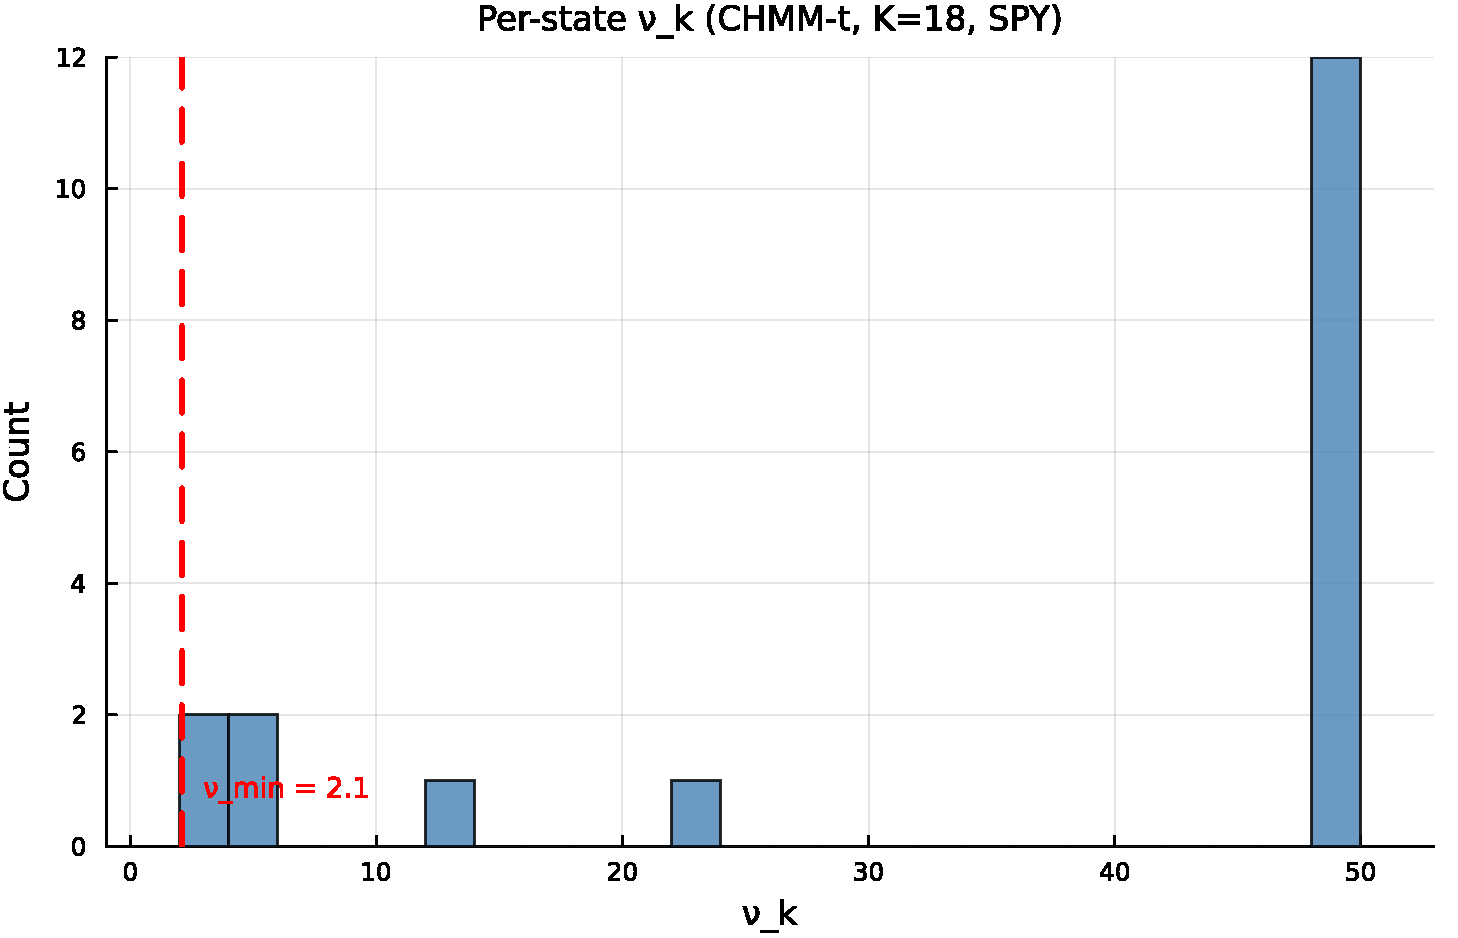
\includegraphics[width=0.75\textwidth]{sections/figs/Fig-v7-nu-Histogram.pdf}
\caption{Per-state degrees-of-freedom $\nu_k$ for the CHMM-t fit at $K = 18$ on SPY IS. The dashed red line marks the lower ECM bracket $\nu_{\min} = 2.1$. Only two states ($\nu_2 = 2.19$, $\nu_4 = 2.10$) sit near the lower bracket; the median $\nu_k$ is at the upper bracket.}
\label{fig:nu_hist}
\end{figure}

Table~\ref{tab:nu_bracket} reports the seven-metric panel for CHMM-t fits whose ECM bracket lower bound is lifted from $\nu_{\min} = 2.1$ through $\{2.5, 3.0, 4.0\}$, plus the Gaussian limit ($\nu = \infty$, equivalent to CHMM-N).
Lifting the bracket does not reduce the in-sample kurtosis overshoot: the simulated kurtosis moves within the $12.5$--$14.0$ band across bracket floors and only collapses to $5.05$ in the full Gaussian limit.
The overshoot is therefore a feature of the Student-t emission family at $K = 18$ and not a lower-bracket artefact.

\begin{table}[h]
\centering
\small
\caption{CHMM-t $\nu_{\min}$ bracket sensitivity at $K = 18$ on SPY (seed = 20260420, 1000 paths).}
\label{tab:nu_bracket}
\begin{tabular}{l cc cc cc c c c}
\toprule
$\nu_{\min}$ & KS IS & AD IS & KS OoS & AD OoS & Kurt IS & Kurt OoS & ACF-MAE & $W_1$ & $H$ \\
\midrule
$2.1$     & 95.7 & 90.2 & 86.2 & 82.0 & 13.95 & 10.08 & 0.0546 & 0.100 & 0.0759 \\
$2.5$     & 95.8 & 90.6 & 84.2 & 79.1 & 15.12 & 10.34 & 0.0547 & 0.100 & 0.0759 \\
$3.0$     & 93.8 & 89.5 & 85.3 & 80.4 & 12.25 & 9.65  & 0.0548 & 0.099 & 0.0760 \\
$4.0$     & 95.5 & 89.5 & 85.0 & 80.3 & 13.25 & 9.39  & 0.0550 & 0.101 & 0.0759 \\
$\infty$ (Gauss) & 94.1 & 86.7 & 84.2 & 75.5 & 5.03  & 4.46 & 0.0510 & 0.110 & 0.0809 \\
\midrule
\textit{Observed} & -- & -- & -- & -- & 7.68 & 5.29 & -- & -- & -- \\
\bottomrule
\end{tabular}
\end{table}

\subsection{Ryd\'en K = 2 Replication}
\label{sec:ryden_replication}

Table~\ref{tab:ryden_init} reports the direct replication of Ryd\'en et al.'s 1998 $K = 2$ setting on SPY IS under both initialization strategies, as discussed in Section~\ref{sec:discussion}.
The quantile-based initialization used in the main body is row 1; five independent random-seed initializations are rows 2--6.
Random init here draws per-state $(\mu_k, \sigma_k)$ from a moderate perturbation of the sample moments, which is representative of the random-init practice common in the 1990s HMM literature.

\begin{table}[h]
\centering
\small
\caption{Ryd\'en replication: $K = 2$ CHMM-N on SPY IS under quantile vs random initialization (seed sub-index varies the random init).}
\label{tab:ryden_init}
\begin{tabular}{l c c c c c}
\toprule
Init & KS IS (\%) & AD IS (\%) & ACF-MAE & Kurt IS & KS OoS (\%) \\
\midrule
Quantile (main body) & 79.0 & 71.5 & 0.0501 & 2.57 & 72.4 \\
Random seed = 1      & 78.7 & 70.7 & 0.0502 & 2.57 & 73.2 \\
Random seed = 7      & 75.3 & 69.6 & 0.0498 & 2.56 & 74.0 \\
Random seed = 42     & 77.6 & 70.0 & 0.0498 & 2.59 & 71.8 \\
Random seed = 100    & 76.2 & 69.4 & 0.0500 & 2.59 & 72.3 \\
Random seed = 2024   & 76.4 & 69.8 & 0.0499 & 2.54 & 72.9 \\
\bottomrule
\end{tabular}
\end{table}

The key observation is that ACF-MAE is essentially constant at $\approx 0.050$ across all six rows, matching the $K = 18$ CHMM-N of the main body.
In-sample KS pass rate remains below the $K = 18$ operating point ($75.3$--$79.0\%$) because two Gaussian components cannot tile the full multi-regime return distribution.
The combination confirms that the Ryd\'en low-$K$ limitation is a distributional (not temporal) artefact: the ACF is already well reproduced at $K = 2$, and it is distributional fidelity that drives the preference for $K = 18$.

\subsection{OoS KS Test-Power Calibration}
\label{sec:ks_power}

Table~\ref{tab:ks_power} reports the two-sample KS test-power calibration used to anchor the OoS KS pass rates of Section~\ref{sec:oos}.
For each of $1{,}000$ Monte Carlo replications (seed = 20260420), a simulated series of length $T_{\text{OoS}} = 572$ is drawn from each of three reference generators and tested against the observed OoS series using the same $\alpha = 0.05$ threshold as the main-body pass-rate metric.

\begin{table}[h]
\centering
\small
\caption{OoS KS pass-rate calibration (1000 replications, seed = 20260420).}
\label{tab:ks_power}
\begin{tabular}{l c}
\toprule
Reference generator & Pass rate (\%) \\
\midrule
I.i.d.\ resamples of $R_{\text{OoS}}$ at length $T_{\text{OoS}} = 572$ (known-correct ceiling) & 100.0 \\
I.i.d.\ resamples of $R_{\text{IS}}$ at length $T_{\text{OoS}} = 572$ (nearly correct)          & 90.0  \\
Gaussian$(\hat\mu_{\text{IS}}, \hat\sigma_{\text{IS}})$ at length $T_{\text{IS}}$ (negative control) & 0.0 \\
\bottomrule
\end{tabular}
\end{table}

The $90.0\%$ "nearly correct" rate is the practical ceiling for the CHMM OoS KS pass rates reported in Section~\ref{sec:oos} ($80$--$84\%$); the $0\%$ rate on the Gaussian misspecified generator confirms that the KS test retains ample power at IS length to reject clearly wrong generators.

\subsection{Walk-Forward Rolling-Window Re-Estimation (Pipeline A)}
\label{sec:walk_forward}

This robustness check lives inside Pipeline A: the CHMM-N is still fit per ticker independently, only the fit window rolls forward. It does not introduce cross-asset coupling, and therefore should not be interpreted alongside the Pipeline B results in Section~\ref{sec:cross_asset}. Table~\ref{tab:walk_forward} reports the quarterly walk-forward re-estimation results referenced in Section~\ref{sec:cross_asset_univariate}.
The walk-forward protocol refits the CHMM-N every $63$ trading days (one quarter) across the $572$-day OoS window, feeding the realized returns of the prior quarter into the training set before each refit.
The rolling protocol recovers a modest $\sim 1$ percentage point on JNJ and a substantial $\sim 15$ percentage points on JPM relative to the fixed-IS baseline, confirming that the stationarity assumption is the principal contributor to the JPM OoS gap while JNJ's OoS gap is already small under the fixed fit.

\begin{table}[h]
\centering
\small
\caption{\textbf{Walk-forward (quarterly CHMM-N refit) vs fixed-IS CHMM-N on JNJ and JPM} (Pipeline A, per-ticker independent fits; walk-forward only rolls the fit window, it does not introduce cross-asset dependence). $K = 18$, 1000 simulated paths per (ticker, mode), seed = 20260420. IS window 2014-01-03 through 2024-01-03; OoS window 2024-01-04 through 2026-04-17 ($T_{\text{OoS}} = 572$). The walk-forward mode refits the CHMM-N every 63 trading days across the OoS window, feeding each completed quarter's realized returns back into the training set before the next refit. Columns report percent KS / AD pass rate at $\alpha = 0.05$, excess kurtosis, ACF-MAE of $|G_t|$, Wasserstein-1, and Hellinger distance.}
\label{tab:walk_forward}
\begin{tabular}{l cc cc cc c c c}
\toprule
Mode & KS IS & AD IS & KS OoS & AD OoS & Kurt IS & Kurt OoS & ACF-MAE & $W_1$ & $H$ \\
\midrule
JNJ fixed-IS      & 99.3 & 98.2 & 94.0 & 92.1 & 5.46 & 4.98 & 0.0322 & 0.095 & 0.0786 \\
JNJ walk-forward  & 99.3 & 98.2 & 94.9 & 91.3 & 5.46 & 5.14 & 0.0322 & 0.095 & 0.0786 \\
JPM fixed-IS      & 96.6 & 94.4 & 49.0 & 48.6 & 7.33 & 6.31 & 0.0449 & 0.165 & 0.0875 \\
JPM walk-forward  & 96.6 & 94.4 & 64.3 & 63.6 & 7.33 & 5.96 & 0.0449 & 0.165 & 0.0875 \\
\bottomrule
\end{tabular}
\end{table}

\subsection{Student-t Copula Profile Log-Likelihood (Pipeline B)}
\label{sec:copula_profile_supp}

Figure~\ref{fig:copula_profile} plots the profile log-likelihood of the Student-t copula used inside Pipeline B, computed on the six-asset SPY cross-section over the grid $\nu \in \{2, 3, 4, 5, 6, 8, 10, 15, 20, 30\}$ used in Section~\ref{sec:cross_asset}.
The curve is smooth and single-peaked, with $\nu^{*} = 6$ attaining the maximum profile log-likelihood ($6157.47$), and the neighbouring grid points $\nu = 5$ ($6143.37$) and $\nu = 8$ ($6148.37$) each within $15$ profile-log-likelihood units of the peak, indicating a shallow-but-clean optimum that agrees with the $4$--$10$ range typically reported for equity-portfolio Student-t copulas in the risk-management literature.

\begin{figure}[h]
\centering
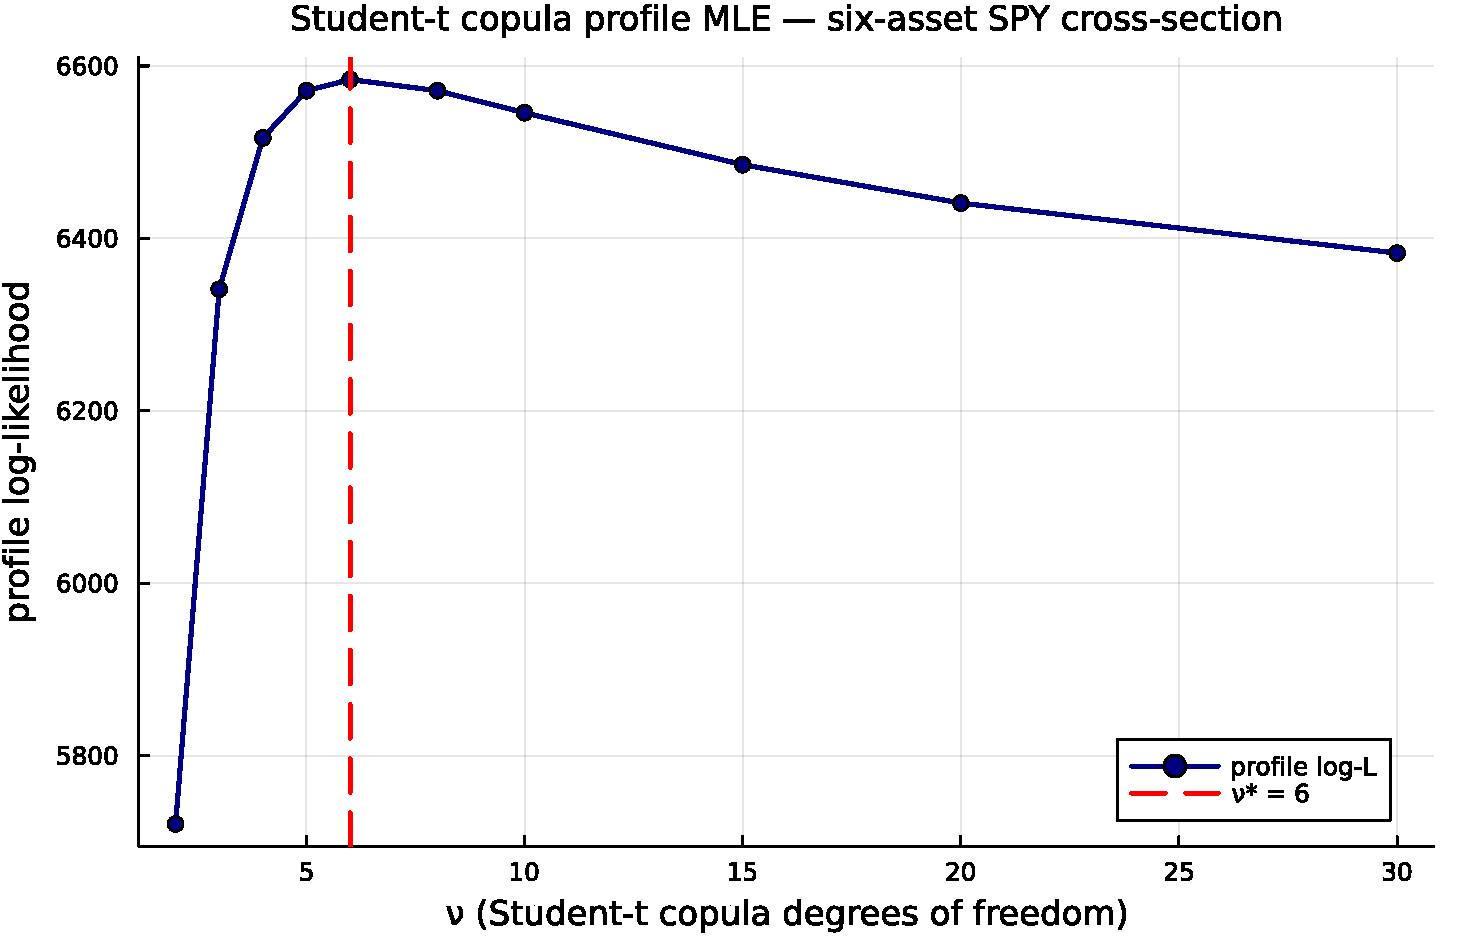
\includegraphics[width=0.70\textwidth]{sections/figs/Fig-v7-Copula-Profile.pdf}
\caption{\textbf{Profile log-likelihood of the Student-t copula} used inside Pipeline B on the six-asset SPY cross-section (SPY, NVDA, JNJ, JPM, AAPL, QQQ; IS window 2014-01-03 through 2024-01-03). The vertical axis is the profile log-likelihood evaluated at each degrees-of-freedom value $\nu$ on the grid $\{2, 3, 4, 5, 6, 8, 10, 15, 20, 30\}$; the dashed red line marks the profile MLE $\nu^{*} = 6$ (peak value 6157.47). The CHMM-N marginals are held fixed at the Pipeline A per-asset fits while $\nu$ is varied.}
\label{fig:copula_profile}
\end{figure}

\subsection{Block-Bootstrap Baseline}
\label{sec:block_bootstrap_supp}

Table~\ref{tab:block_bootstrap} reports the full seven-metric panel for the stationary block bootstrap at block length $b = 10$ trading days, the temporally-aware non-parametric baseline added to Table~\ref{tab:model_comparison}.

\begin{table}[h]
\centering
\small
\caption{Stationary block bootstrap (block length $b = 10$ trading days) on SPY (1000 paths, seed = 20260420).}
\label{tab:block_bootstrap}
\begin{tabular}{l cc cc c c c c}
\toprule
Window & KS & AD & Kurt & ACF-MAE & $W_1$ & $H$ & Cov \\
\midrule
IS  & 99.2 & 96.4 & 7.07 & 0.0568 & 0.092 & 0.0534 & 100.0 \\
OoS & 87.5 & 86.4 & 5.34 & 0.0512 & 0.225 & 0.1570 & 86.9  \\
\bottomrule
\end{tabular}
\end{table}

\subsection{Discrete HMM with Bin-Conditional Student-t Emissions}
\label{sec:bin_t_supp}

Table~\ref{tab:bin_t} reports the full seven-metric panel for the Bin-T NJ variant referenced in Section~\ref{sec:model_comparison}: the discrete NJ transition matrix with $K_{\text{disc}} = 13$ quantile bins, but with each bin emitting from a bin-conditional Student-t density rather than from the bin centroid.

\begin{table}[h]
\centering
\small
\caption{Discrete HMM with bin-conditional Student-t emissions on SPY (no jumps, $K_{\text{disc}} = 13$, 1000 paths, seed = 20260420).}
\label{tab:bin_t}
\begin{tabular}{l cc cc c c c c}
\toprule
Window & KS & AD & Kurt & ACF-MAE & $W_1$ & $H$ & Cov \\
\midrule
IS  & 95.4 & 92.1 & 26.18 & 0.0619 & 0.116 & 0.0929 & 89.9 \\
OoS & 86.7 & 93.2 & 10.76 & 0.0538 & 0.177 & 0.1614 & 93.9 \\
\bottomrule
\end{tabular}
\end{table}

The bin-conditional Student-t fit picks $\nu \approx 2.71$ for the two extreme bins (bins $1$ and $13$, corresponding to the lower and upper quantile tails of the IS distribution) and $\nu = 50$ (upper bracket) for the eleven central bins, which explains both the large in-sample simulated kurtosis ($26.18$) and the very thin-scale central bins ($\sigma$ $\sim$ $0.06$--$0.28$).



\subsection{GRU Deep-Generative Baseline}
\label{sec:gru_supp}

Architecture and training details for the GRU baseline used in
Section~\ref{sec:model_comparison} are summarised here.

\begin{itemize}
    \item \textbf{Architecture.} A single-layer Gated Recurrent Unit (GRU)
    with hidden dimension $H = 32$ followed by a Dense head with two
    outputs $(\mu_t, \log \sigma_t)$. Input is a single feature (the
    standardised return) over a context window of $w = 20$ trading days.

    \item \textbf{Loss.} Per-window negative log-likelihood of a Gaussian
    next-step density, equation~\eqref{eq:gru_nll}.

    \item \textbf{Optimiser.} Adam, learning rate $1.0 \times 10^{-3}$.

    \item \textbf{Training schedule.} $20$ epochs, full pass per epoch
    over $T_{\text{IS}} - w$ training windows, randomly shuffled at each
    epoch.

    \item \textbf{Numerical stability.} $\log \sigma_t$ is clamped to
    $[-6, 4]$ inside the loss to prevent gradient explosion when the
    network attempts to assign vanishingly-small variance to extreme
    observations.

    \item \textbf{Pre-processing.} The input return series is standardised
    by its in-sample mean and standard deviation; predictions are
    re-scaled back at sampling time.

    \item \textbf{Synthesis.} The trailing $w$ in-sample returns seed the
    recurrence; for each generation step the predicted Gaussian is
    sampled, the sample is appended to the context window, and the
    procedure rolls forward. The first $64$ steps are discarded as
    burn-in.

    \item \textbf{Implementation.} Julia using \texttt{Flux.jl}
    \cite{innes2018flux} with the \texttt{Optimisers.Adam} state.
    Random seed for weight initialisation, training shuffling, and per-path
    sampling: $V7\_SEED = 20260420$ with deterministic per-path sub-seeds.
\end{itemize}

The trained model is callable through the same
\texttt{simulate\_gru(model, n\_steps; seed\_window)} interface as the
CHMM and discrete-HMM models, so the seven-metric panel evaluates the GRU
on byte-identical windows to the other generators.

\begin{table}[h]
\centering
\small
\caption{GRU deep-generative baseline on SPY (single-layer, hidden $H=32$, window $w=20$, $20$ epochs, Adam $\eta=10^{-3}$, $1{,}000$ paths, seed = 20260420). Final training NLL: $0.2005$.}
\label{tab:gru}
\begin{tabular}{l cc c c c c c}
\toprule
Window & KS & AD & Kurt & ACF-MAE & $W_1$ & $H$ & Cov \\
\midrule
IS  & 18.1 & 13.7 & 2.85 & 0.0518 & 0.196 & 0.0966 & 37.4 \\
OoS & 52.5 & 55.0 & 2.21 & 0.0500 & 0.293 & 0.1603 & 69.7 \\
\bottomrule
\end{tabular}
\end{table}

\subsection{Per-Ticker OoS Price-Simulation Figures (Unconditional CHMM)}
\label{sec:price_sim_oos_appendix}

This appendix collects the per-ticker price-fan and terminal-distribution figures deferred from Section~\ref{sec:price_sim_oos} for the four non-body tickers JNJ, JPM, AAPL, and QQQ.
All figures use the same plotting conventions as Figure~\ref{fig:price_fan_spy} in the main body: blue shaded bands are the $5$--$95\%$ and $25$--$75\%$ quantile envelopes of the $500$ simulated paths, blue solid line is the simulated median, red solid line is the observed OoS price track.
Terminal histograms follow the conventions of Figure~\ref{fig:price_terminal_hists}.
Summary metrics for all four tickers are in Tables~\ref{tab:price_sim_oos} and~\ref{tab:price_sim_path_metrics} in the main body.

\begin{figure}[h]
\centering
\begin{subfigure}[t]{0.32\textwidth}
    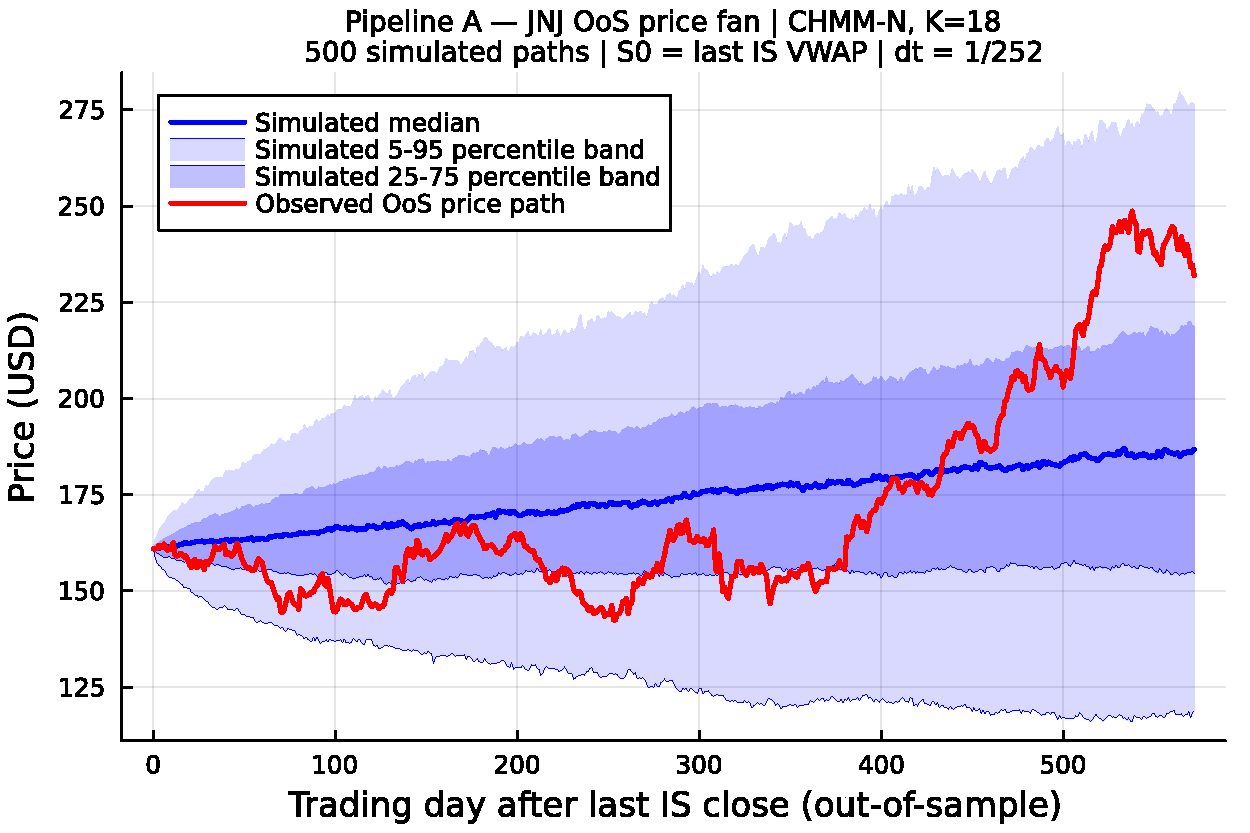
\includegraphics[width=\textwidth]{sections/figs/Fig-JNJ-PriceFan-N.pdf}
    \caption{CHMM-N.}
\end{subfigure}
\begin{subfigure}[t]{0.32\textwidth}
    
\includegraphics[width=\textwidth]{sections/figs/Fig-JNJ-PriceFan-t.pdf}
    \caption{CHMM-t.}
\end{subfigure}
\begin{subfigure}[t]{0.32\textwidth}
    
\includegraphics[width=\textwidth]{sections/figs/Fig-JNJ-PriceFan-L.pdf}
    \caption{CHMM-L.}
\end{subfigure}
\caption{JNJ out-of-sample price fan, unconditional CHMM sampler.}
\label{fig:price_fan_jnj_appendix}
\end{figure}

\begin{figure}[h]
\centering
\begin{subfigure}[t]{0.32\textwidth}
    
\includegraphics[width=\textwidth]{sections/figs/Fig-JNJ-TerminalDist-N.pdf}
    \caption{CHMM-N.}
\end{subfigure}
\begin{subfigure}[t]{0.32\textwidth}
    
\includegraphics[width=\textwidth]{sections/figs/Fig-JNJ-TerminalDist-t.pdf}
    \caption{CHMM-t.}
\end{subfigure}
\begin{subfigure}[t]{0.32\textwidth}
    
\includegraphics[width=\textwidth]{sections/figs/Fig-JNJ-TerminalDist-L.pdf}
    \caption{CHMM-L.}
\end{subfigure}
\caption{JNJ terminal-price distribution, unconditional CHMM sampler.}
\label{fig:terminal_jnj_appendix}
\end{figure}

\begin{figure}[h]
\centering
\begin{subfigure}[t]{0.32\textwidth}
    
\includegraphics[width=\textwidth]{sections/figs/Fig-JPM-PriceFan-N.pdf}
    \caption{CHMM-N.}
\end{subfigure}
\begin{subfigure}[t]{0.32\textwidth}
    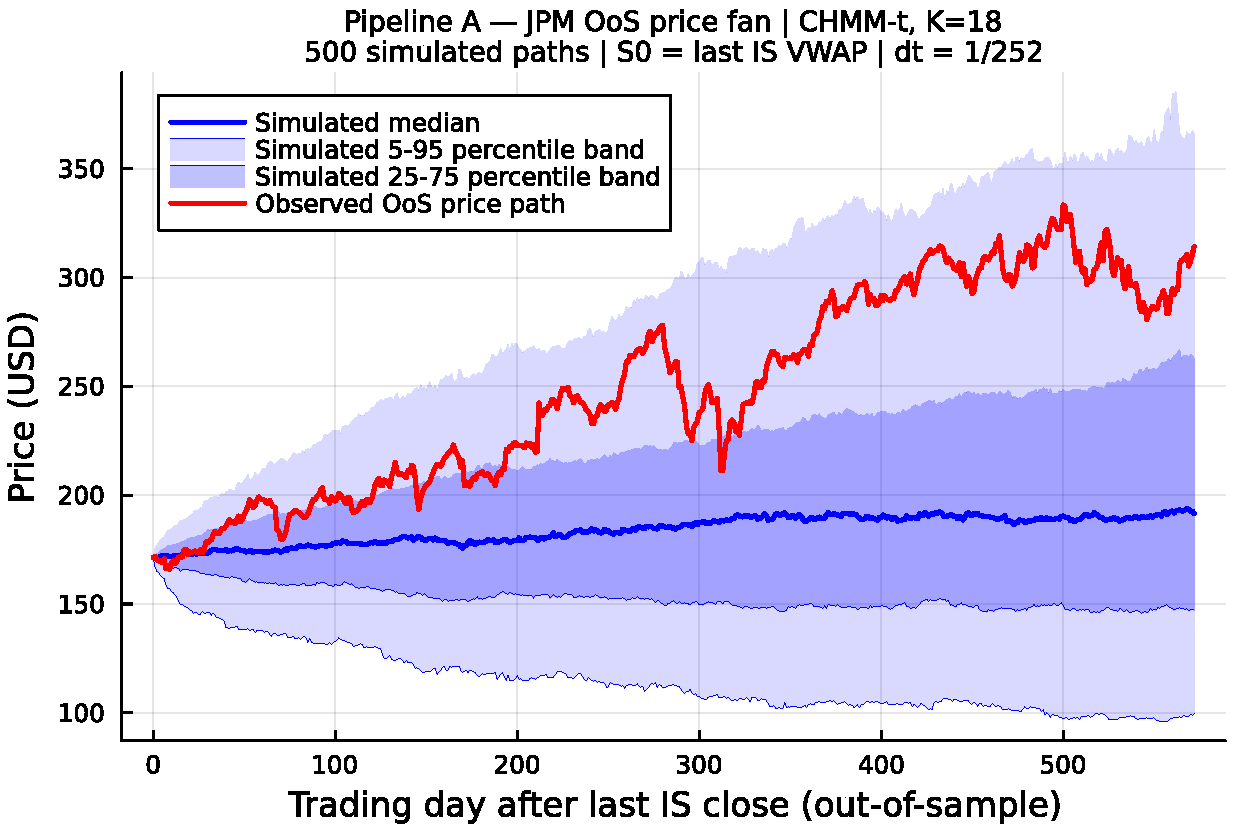
\includegraphics[width=\textwidth]{sections/figs/Fig-JPM-PriceFan-t.pdf}
    \caption{CHMM-t.}
\end{subfigure}
\begin{subfigure}[t]{0.32\textwidth}
    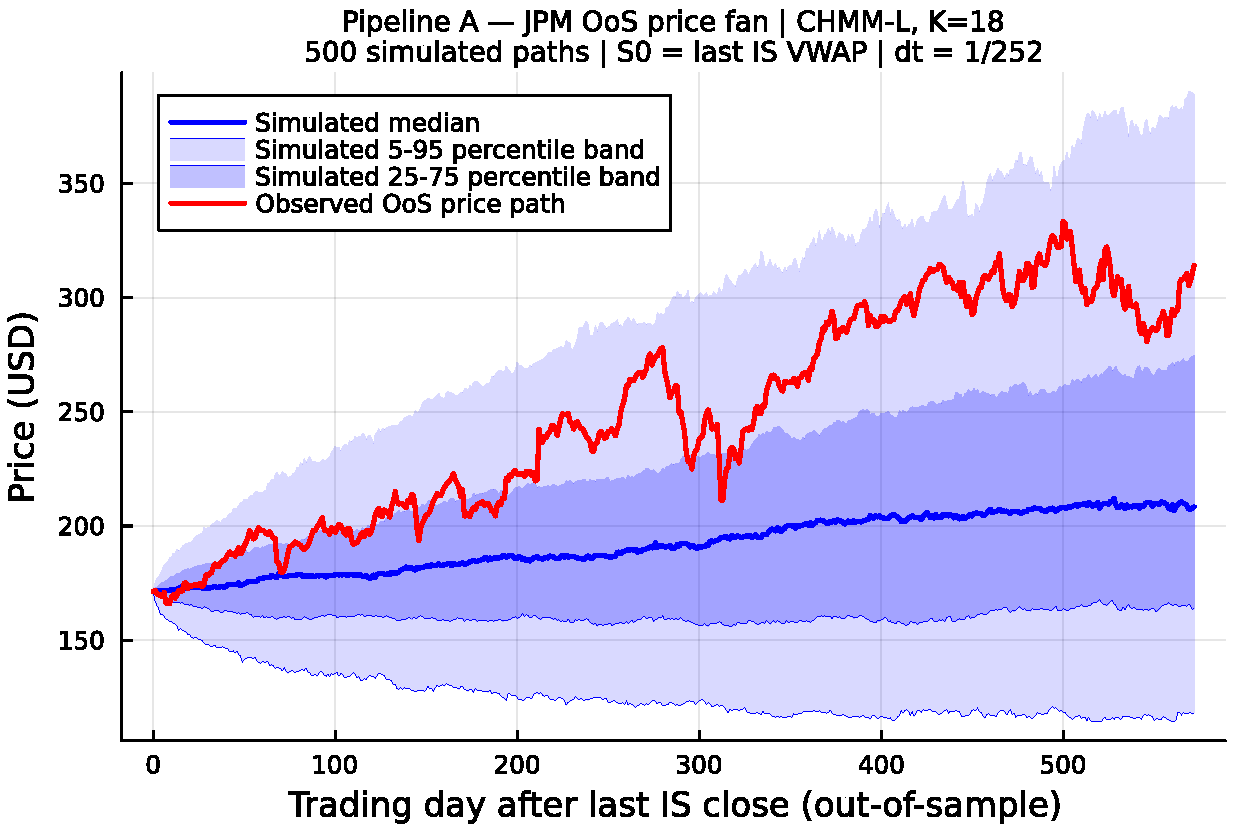
\includegraphics[width=\textwidth]{sections/figs/Fig-JPM-PriceFan-L.pdf}
    \caption{CHMM-L.}
\end{subfigure}
\caption{JPM out-of-sample price fan, unconditional CHMM sampler.}
\label{fig:price_fan_jpm_appendix}
\end{figure}

\begin{figure}[h]
\centering
\begin{subfigure}[t]{0.32\textwidth}
    
\includegraphics[width=\textwidth]{sections/figs/Fig-JPM-TerminalDist-N.pdf}
    \caption{CHMM-N.}
\end{subfigure}
\begin{subfigure}[t]{0.32\textwidth}
    
\includegraphics[width=\textwidth]{sections/figs/Fig-JPM-TerminalDist-t.pdf}
    \caption{CHMM-t.}
\end{subfigure}
\begin{subfigure}[t]{0.32\textwidth}
    
\includegraphics[width=\textwidth]{sections/figs/Fig-JPM-TerminalDist-L.pdf}
    \caption{CHMM-L.}
\end{subfigure}
\caption{JPM terminal-price distribution, unconditional CHMM sampler.}
\label{fig:terminal_jpm_appendix}
\end{figure}

\begin{figure}[h]
\centering
\begin{subfigure}[t]{0.32\textwidth}
    
\includegraphics[width=\textwidth]{sections/figs/Fig-AAPL-PriceFan-N.pdf}
    \caption{CHMM-N.}
\end{subfigure}
\begin{subfigure}[t]{0.32\textwidth}
    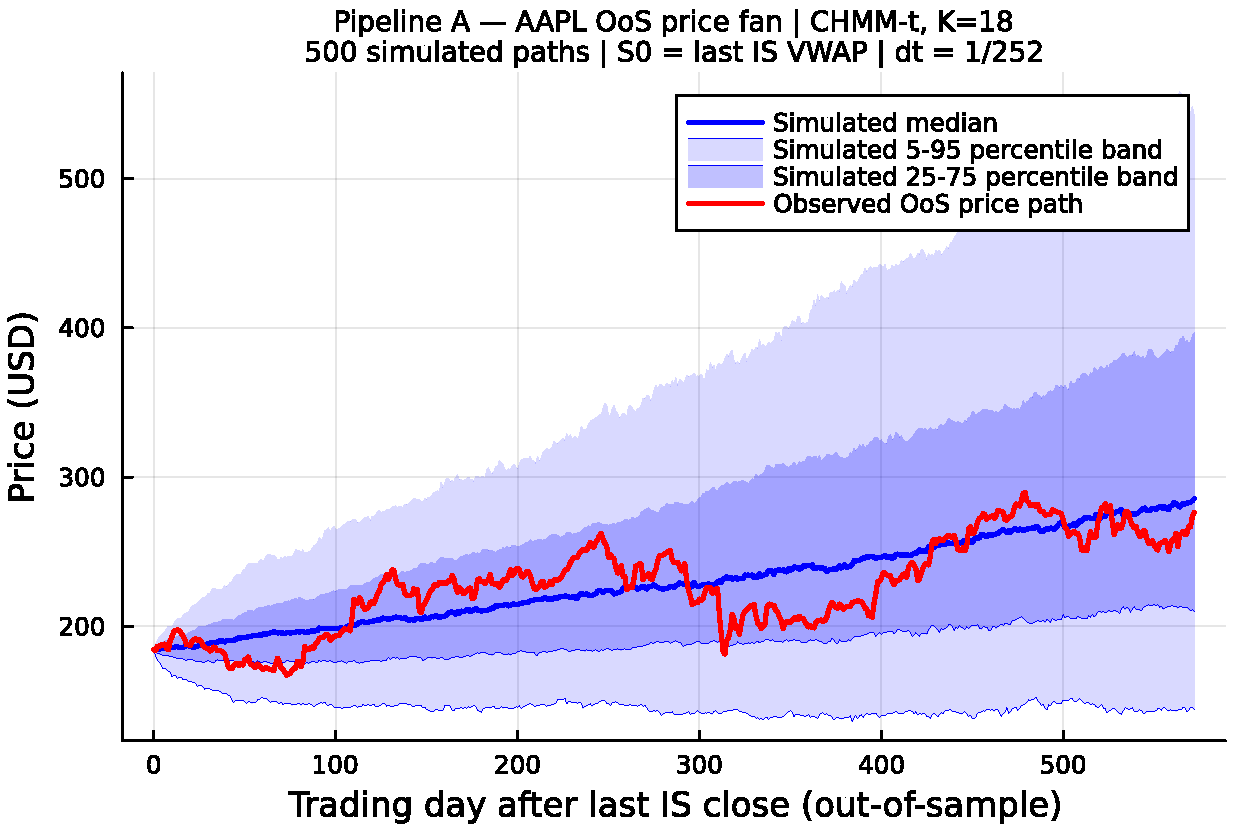
\includegraphics[width=\textwidth]{sections/figs/Fig-AAPL-PriceFan-t.pdf}
    \caption{CHMM-t.}
\end{subfigure}
\begin{subfigure}[t]{0.32\textwidth}
    
\includegraphics[width=\textwidth]{sections/figs/Fig-AAPL-PriceFan-L.pdf}
    \caption{CHMM-L.}
\end{subfigure}
\caption{AAPL out-of-sample price fan, unconditional CHMM sampler.}
\label{fig:price_fan_aapl_appendix}
\end{figure}

\begin{figure}[h]
\centering
\begin{subfigure}[t]{0.32\textwidth}
    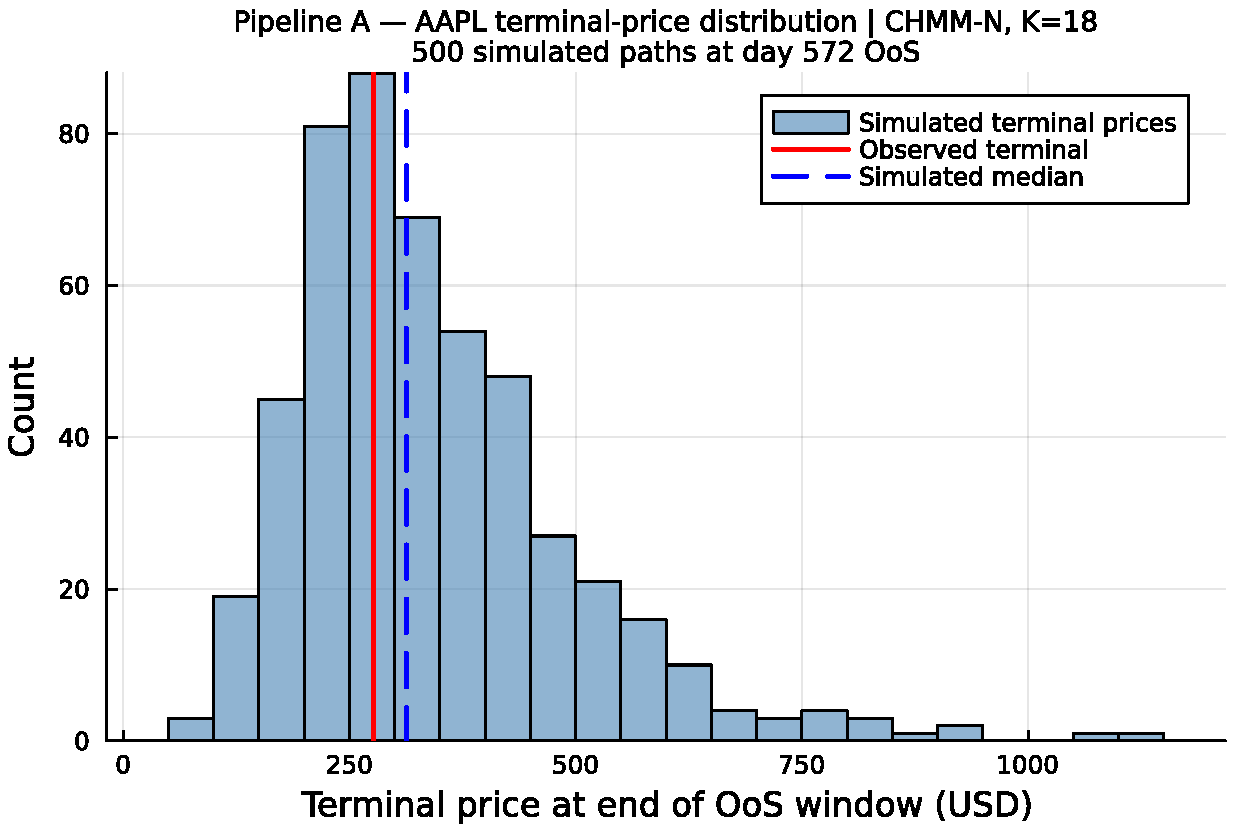
\includegraphics[width=\textwidth]{sections/figs/Fig-AAPL-TerminalDist-N.pdf}
    \caption{CHMM-N.}
\end{subfigure}
\begin{subfigure}[t]{0.32\textwidth}
    
\includegraphics[width=\textwidth]{sections/figs/Fig-AAPL-TerminalDist-t.pdf}
    \caption{CHMM-t.}
\end{subfigure}
\begin{subfigure}[t]{0.32\textwidth}
    
\includegraphics[width=\textwidth]{sections/figs/Fig-AAPL-TerminalDist-L.pdf}
    \caption{CHMM-L.}
\end{subfigure}
\caption{AAPL terminal-price distribution, unconditional CHMM sampler.}
\label{fig:terminal_aapl_appendix}
\end{figure}

\begin{figure}[h]
\centering
\begin{subfigure}[t]{0.32\textwidth}
    
\includegraphics[width=\textwidth]{sections/figs/Fig-QQQ-PriceFan-N.pdf}
    \caption{CHMM-N.}
\end{subfigure}
\begin{subfigure}[t]{0.32\textwidth}
    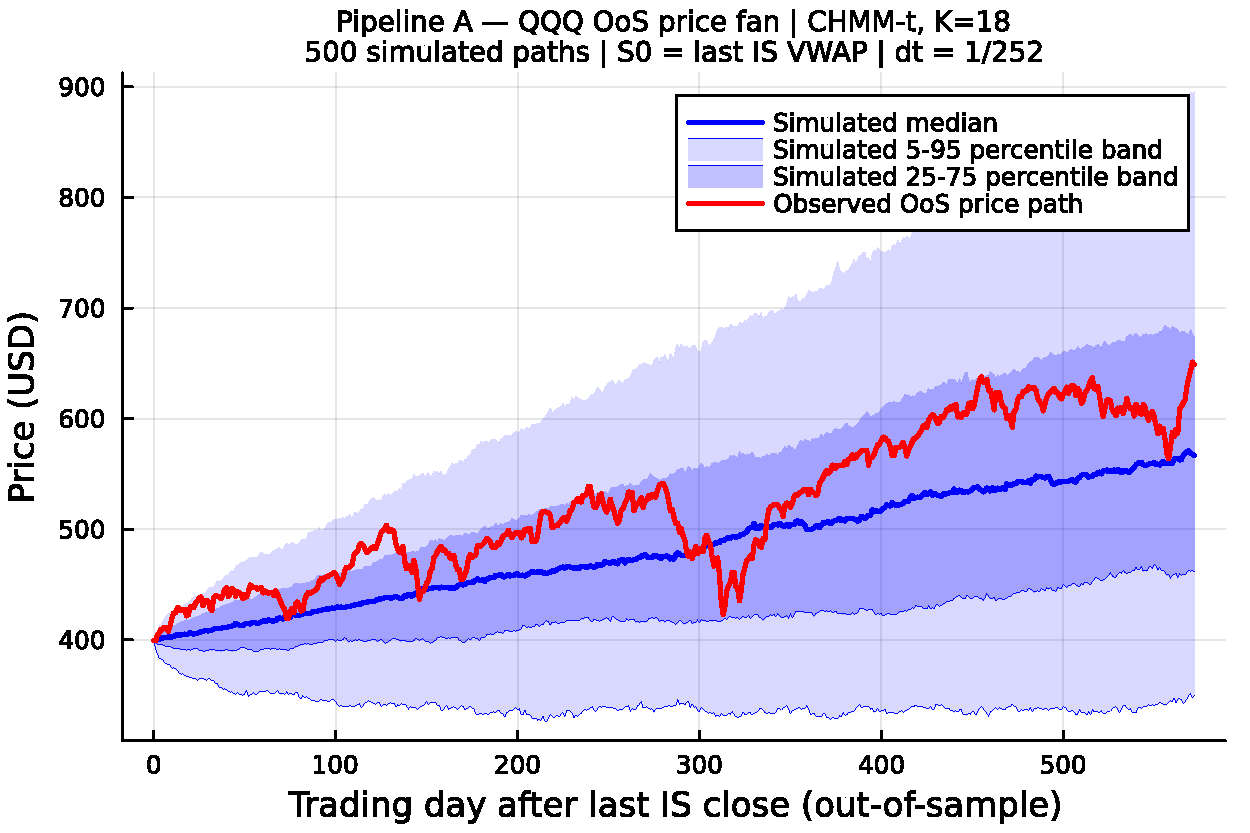
\includegraphics[width=\textwidth]{sections/figs/Fig-QQQ-PriceFan-t.pdf}
    \caption{CHMM-t.}
\end{subfigure}
\begin{subfigure}[t]{0.32\textwidth}
    
\includegraphics[width=\textwidth]{sections/figs/Fig-QQQ-PriceFan-L.pdf}
    \caption{CHMM-L.}
\end{subfigure}
\caption{QQQ out-of-sample price fan, unconditional CHMM sampler.}
\label{fig:price_fan_qqq_appendix}
\end{figure}

\begin{figure}[h]
\centering
\begin{subfigure}[t]{0.32\textwidth}
    
\includegraphics[width=\textwidth]{sections/figs/Fig-QQQ-TerminalDist-N.pdf}
    \caption{CHMM-N.}
\end{subfigure}
\begin{subfigure}[t]{0.32\textwidth}
    
\includegraphics[width=\textwidth]{sections/figs/Fig-QQQ-TerminalDist-t.pdf}
    \caption{CHMM-t.}
\end{subfigure}
\begin{subfigure}[t]{0.32\textwidth}
    
\includegraphics[width=\textwidth]{sections/figs/Fig-QQQ-TerminalDist-L.pdf}
    \caption{CHMM-L.}
\end{subfigure}
\caption{QQQ terminal-price distribution, unconditional CHMM sampler.}
\label{fig:terminal_qqq_appendix}
\end{figure}




\end{document}
